\documentclass [a4paper,12pt]{article}
\usepackage {graphicx}
\usepackage {intfpc}
\usepackage {longtable}
%\usepackage {float}
\usepackage{listings}
\lstset{language=Delphi}
\lstset{basicstyle=\sffamily\small}
\lstset{commentstyle=\itshape}
\lstset{keywordstyle=\bfseries}
\lstset{frame=tb}
% eats mem for longtable, but speeds up. Set to 10 for minimal mem req.
\setcounter{LTchunksize}{200}
% right aligned longtables
\setlength\LTleft{0pt}
\setlength\LTright\fill
%\restylefloat{table}
%\restylefloat{longtable}
%\squeezetable
\setcounter{totalnumber}{10}
% This comes from the MDWTOOLS package and should discourage floating.
\def\textfraction{0.1}
\def\topfraction{0.9}
\def\bottomfraction{0.9}
\def\floatpagefraction{0.7}
\def\fps@figure{htbp}
\def\fpc@longtable{h}


\title{FREE PASCAL}
\title{Free Pascal 1.0.x Internal documentation}
\author{Carl Eric Cod\`{e}re}
\makeindex
\begin{document}
\maketitle
\tableofcontents
\newpage
\listoffigures
\newpage

\textbf{TODO:}
\begin{itemize}
\item Explain architecture of the symbol table + API
\item Describe in detail tsymtable, including all methods and fields
\item Describe in detail procinfo (tprocinfo)
\item Explain how a symbol is inserted into the symbol table (and how alignment requirements are met)
\item Explain pparaitem
\item Explain all symbol table fields
\item Finish all internal routines definitions
\item Architecture of the assembler generators + API
\item Architecture of the PPU file and information
\item Explain systems.pas
\item Compiler DEFINES
\item routine parsing and code generation algorithm
\item (MvdV) OS specific stuff (like hardcoded linker includedirs)
\end{itemize}

\section{Introduction}
\label{sec:introductionappendix}

This document will describe the internal architecture of the Free Pascal
Compiler version 1.0 release. This document is meant to be used as a guide
for those who wish to understand how the compiler was created. Most of the
architecture of the compiler described herein is based on the m68k version
on the compiler, the i386 version of the compiler ressembles closely the
m68k version, but there are subtle differences in the different interfaces.

The architecture, and the different passes of the compiler are shown in
figure \ref{fig1}.

\begin{figure}
\ifpdf
% \epsfig{file=arch1d.pdf,width=\textwidth}
 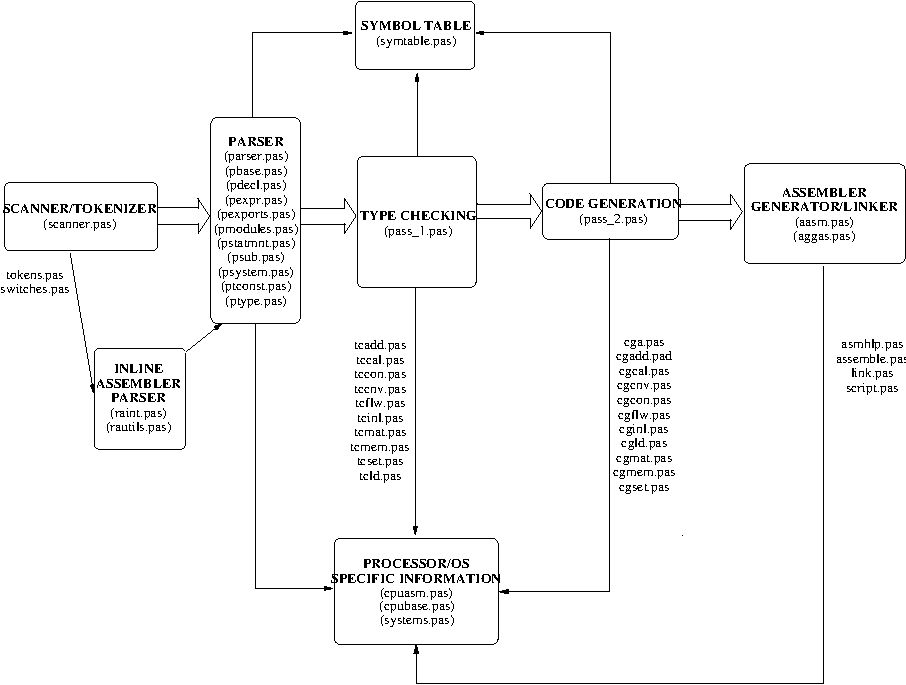
\includegraphics{arch1.pdf}
\else
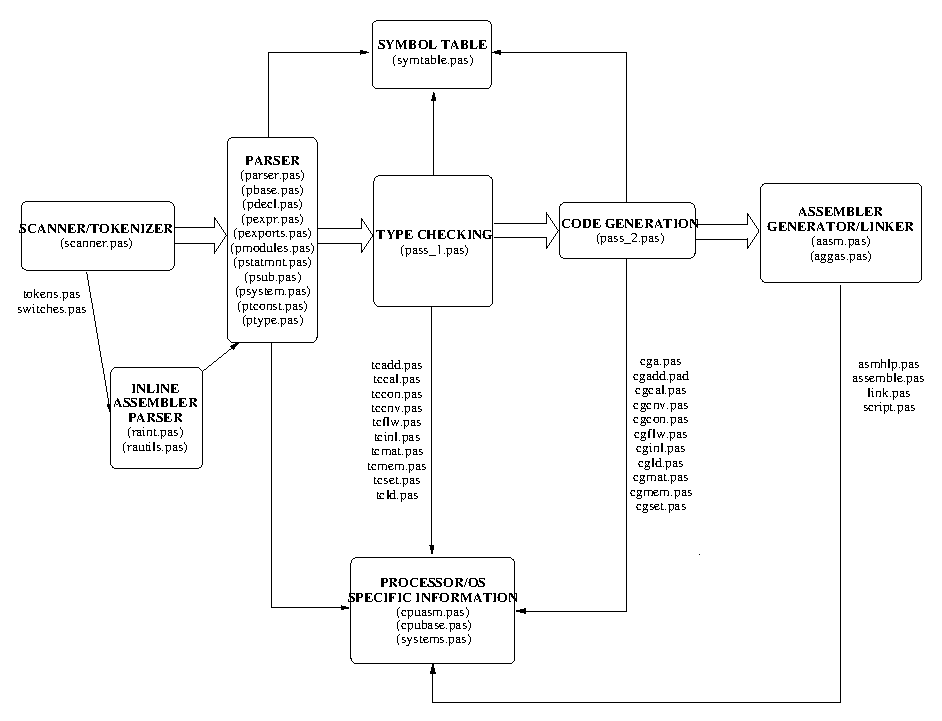
\includegraphics[width=6.45in,height=4.95in]{arch1.eps}
\fi
\caption{TTREE structure}
\label{fig1}
\end{figure}

\section{Scanner / Tokenizer}

The scanner and tokenizer is used to construct an input stream of tokens
which will be fed to the parser. It is in this stage that the preprocessing
is done, that all read compiler directives change the internal state
variables of the compiler, and that all illegal characters found in the
input stream cause an error.

\subsection{Architecture}
\label{subsec:architectureand}

The general architecture of the scanner is show in figure \ref{fig2}

\begin{figure}
\ifpdf
%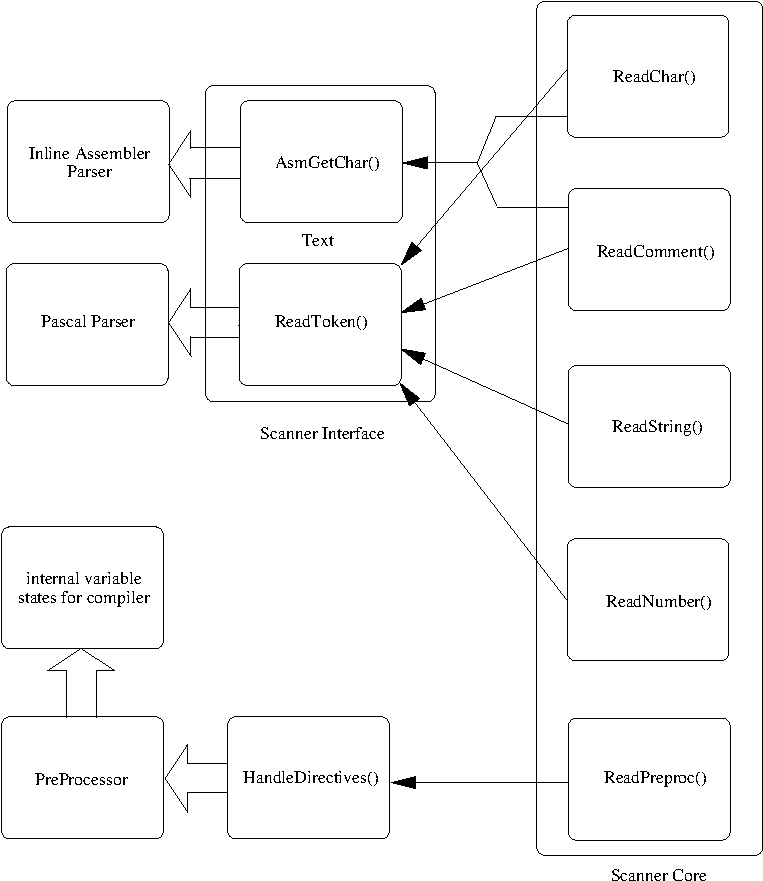
\epsfig{file=arch2.png,width=\textwidth}
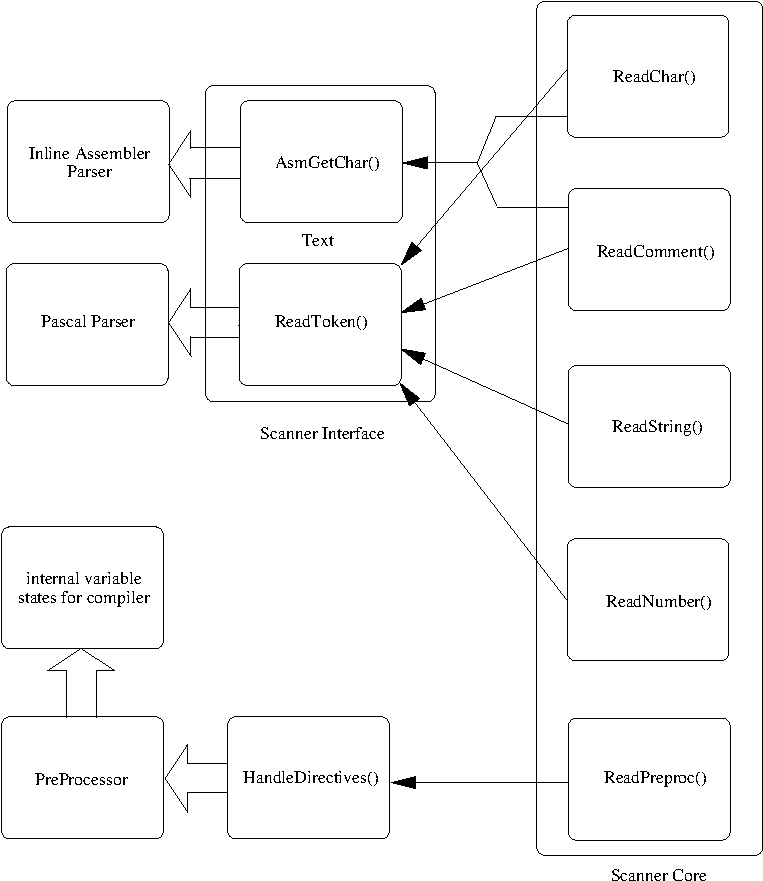
\includegraphics{arch2.pdf}
\else
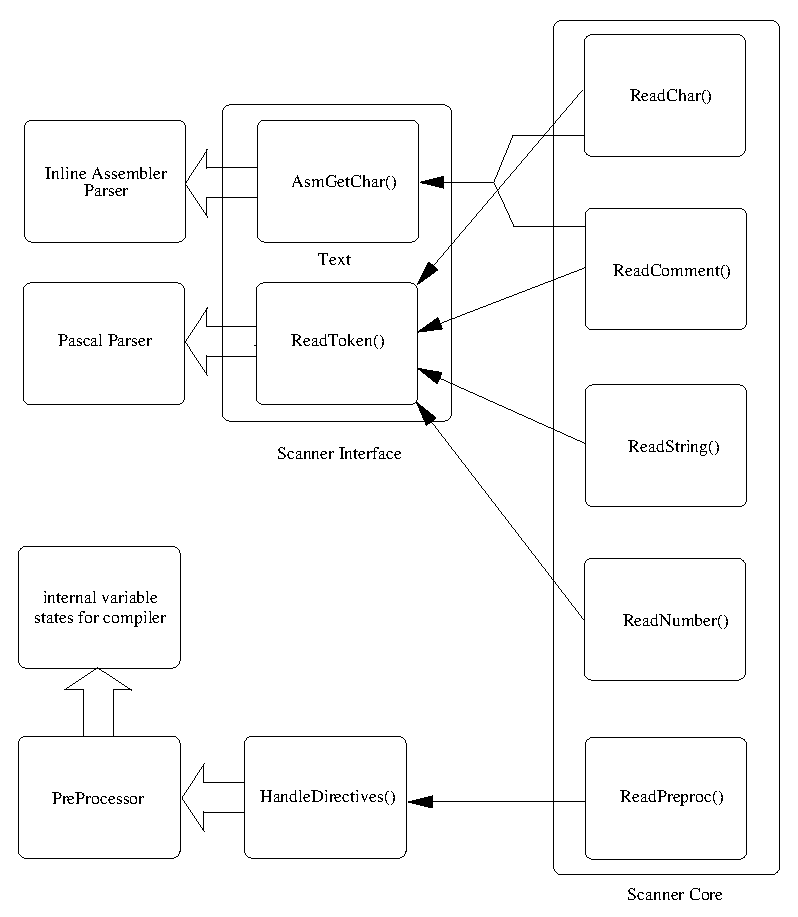
\includegraphics[width=5.87in,height=6.90in]{arch2.eps}
\fi
\caption{Possible tree Local compiler switches (tlocalswitches)}
\label{fig2}
\end{figure}

Several types can be read from the input stream, a string, handled by
readstring(), a numeric value, handled by readnumeric(), comments , compiler
and preprocessor directives.

\subsubsection{Input stream}
\label{subsubsec:input}

The input data is handled via the standard way of handling all the I/O in
the compiler. That is to say, that it is a hook which can be overriden in
\textbf{comphook.pas (do{\_}openinputfile)}, in case where another I/O
method wants to be used.

The default hook uses a non-buffered dos stream contained in
\textbf{files.pas}

\subsubsection{Preprocessor}
\label{subsubsec:preprocessorhook}

The scanner resolves all preprocessor directives and only gives to the
parser the visible parts of the code (such as those which are included in
conditional compilation). Compiler switches and directives are also saved in
global variables while in the preprocessor, therefore this is part is
completely independent of the parser.

\paragraph{Conditional compilation (scandir.inc, scanner.pas)}

The conditional compilation is handled via a preprocessor stack, where each
directive is pushed on a stack, and popped when it is resolved. The actual
implementation of the stack is a linked list of preprocessor directive
items.

\paragraph{Compiler switches (scandir.inc, switches.pas)}

The compiler switches are handled via a lookup table which is linearly
searched. Then another lookup table takes care of setting the appropriate
bit flags and variables in the switches for this compilation process.

\subsection{Scanner interface}
\label{subsec:scanner}

The parser only receives tokens as its input, where a token is a enumeration
which indicates the type of the token, either a reserved word, a special
character, an operator, a numeric constant, string, or an identifier.

Resolution of the string into a token is done via lookup which searches the
string table to find the equivalent token. This search is done using a
binary search algorithm through the string table.

In the case of identifiers, constants (including numeric values), the value
is returned in the \textbf{pattern} string variable , with the appropriate
return value of the token (numeric values are also returned as non-converted
strings, with any special prefix included). In the case of operators, and
reserved words, only the token itself must be assumed to be preserved. The
read input string is assmued to be lost.

Therefore the interface with the parser is with the \textbf{readtoken()}
routine and the \textbf{pattern} variable.

\subsubsection{Routines}
\label{subsubsec:routinese}

\begin{procedure}{ReadToken}
\Declaration
Procedure ReadToken;
\Description
Sets the global variable \textsf{token} to the current token read, and sets
the \textsf{pattern} variable appropriately (if required).
\end{procedure}

% ?? :
%\caption{: Symbol tables in memory}
%\label{tab2}

\subsubsection{Variables}
\label{subsubsec:variablesglobal}

\begin{variable}{Token}
\Description
Var Token : TToken;
\Description
Contains the contain token which was last read by a call to \seep{ReadToken}
\SeeAlso
  \seep{ReadToken}
\end{variable}

%\caption{: Possible symbol table types (tsymboltabletype)}
%\label{tab3}
%\end{table}

\begin{variable}{Pattern}
\Declaration
var Pattern : String;
\Description
Contains the string of the last pattern read by a call to
\seep{ReadToken}
\SeeAlso
 \seep{ReadToken}
\end{variable}

%\caption{: Symbol entry relationships (tsym)}
%\label{tab4}

\subsection{Assembler parser interface}
\label{subsec:assembler}

The inline assembler parser is completely separate from the pascal parser,
therefore its scanning process is also completely independent. The scanner
only takes care of the preprocessor part and comments, all the rest is
passed character per character to the assembler parser via the
\seef{AsmGetChar}() scanner routine.

\begin{function}{AsmGetChar}
\Declaration
Function AsmGetChar: Char;
\Description
Returns the next character in the input stream. 
\end{function}

%\caption{Possible symbol types (TSymTyp)}
%\label{tab5}

\section{The tree}
\label{sec:mylabel2}

\subsection{Architecture}
\label{subsec:architecturenext}

The tree is the basis of the compiler. When the compiler parses statements
and blocks of code, they are converted to a tree representation. This tree
representation is actually a doubly linked list. From this tree the code
generation can easily be implemented.

Assuming that you have the following pascal syntax:

%\lstinline!x := x * y + (6 shl x);!

\begin{center}
$ x := x * y + (6\xspace shl \xspace x);$
\end{center}

The tree structure in picture \ref{fig3} will be built in memory, where each
circle represents an element (a node ) in the tree:

\begin{figure}
\ifpdf
%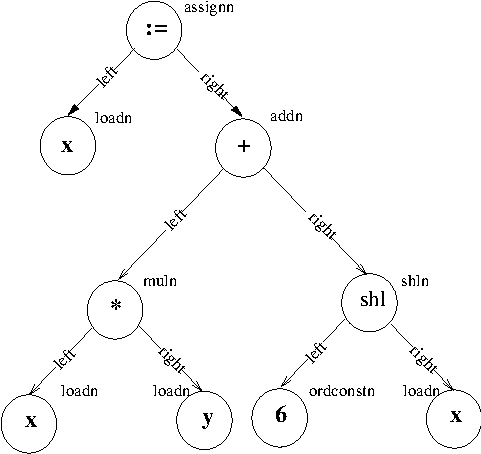
\epsfig{file=arch3.png,width=\textwidth}
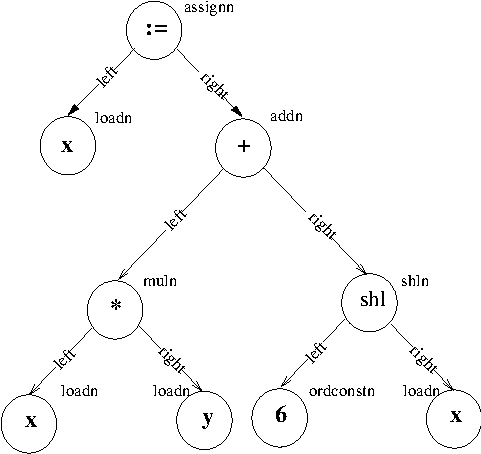
\includegraphics{arch3.pdf}
\else
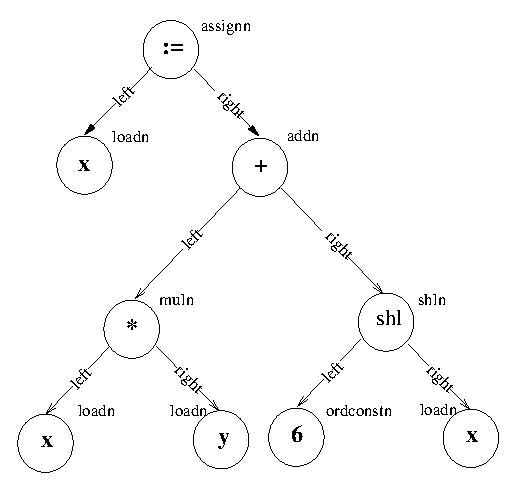
\includegraphics[width=3.88in,height=3.65in]{arch3.eps}
\fi
\caption{Possible variable flags (tvaroptions)}
\label{fig3}
\end{figure}

\subsection{Tree types}

The following tree nodes are possible (of type \textsf{TTreeTyp):}

\begin{longtable}{|l|p{10cm}|}
%{|p{125pt}|p{316pt}|}
\hline
Tree type definition&
Description \\
\hline
\endhead
\hline
\endfoot
\textsf{addn}&
		\textsf{Represents the + operator} \\
\textsf{muln}&
		\textsf{Represents the * operator} \\
\textsf{subn}&
		\textsf{Represents the }\textsf{\textbf{-}}\textsf{ operator} \\
\textsf{divn}&
		\textsf{Represents the }\textsf{\textbf{div}}\textsf{ operator} \\
\textsf{symdifn}&
		\textsf{Represents the }\textsf{\textbf{><}}\textsf{ operator} \\
\textsf{modn}&
		\textsf{Represents the }\textsf{\textbf{mod}}\textsf{ operator} \\
\textsf{assignn}&
		\textsf{Represents the }\textsf{\textbf{:=}}\textsf{ operator (assignment)} \\
\textsf{loadn}&
		\textsf{Represents the use of a variable} \\
\textsf{rangen}&
		\textsf{Represents a numeric range (i.e 0..9)} \\
\textsf{ltn}&
		\textsf{Represents the }\textsf{\textbf{<}}\textsf{ operator} \\
\textsf{lten}&
		\textsf{Represents the }\textsf{\textbf{<=}}\textsf{ operator} \\
\textsf{gtn}&
		\textsf{Represents the }\textsf{\textbf{>}}\textsf{ operator} \\
\textsf{gten}&
		\textsf{Represents the }\textsf{\textbf{>=}}\textsf{ operator} \\
\textsf{equaln}& 	
		\textsf{Represents the = operator} \\
\textsf{unequaln}&
		\textsf{Represents the }\textsf{\textbf{<>}}\textsf{ operator} \\
\textsf{inn}&
		\textsf{Represents the }\textsf{\textbf{in}}\textsf{ operator} \\
\textsf{orn}&
		\textsf{Represents the }\textsf{\textbf{or}}\textsf{ operator} \\
\textsf{xorn}&
		\textsf{Represents the }\textsf{\textbf{xor}}\textsf{ operator} \\
\textsf{shrn}&
		\textsf{Represents the }\textsf{\textbf{shr}}\textsf{ operator} \\
\textsf{shln}&
		\textsf{Represents the }\textsf{\textbf{shl}}\textsf{ operator} \\
\textsf{slashn}&
		\textsf{Represents the / operator} \\
\textsf{andn}&
		\textsf{Represents the }\textsf{\textbf{and}}\textsf{ operator} \\
\textsf{subscriptn}&
		\textsf{Represents a field in an object or record} \\
\textsf{derefn}&
		\textsf{Represents a pointer reference (such as the }\textsf{\textbf{\ }}\textsf{ operator)} \\
\textsf{addrn}&
		\textsf{Represents the }\textsf{\textbf{@}}\textsf{ operator} \\
\textsf{doubleaddrn}&
		\textsf{Represents the }\textsf{\textbf{@@}}\textsf{ operator} \\
\textsf{ordconstn}&
		\textsf{Represents an ordinal constant} \\
\textsf{typeconvn}&
		\textsf{Represents a typecast / type conversion} \\
\textsf{calln}&
		\textsf{Represents a routine call} \\
\textsf{callparan}&
		\textsf{Represents a parameter passed to a routine} \\
\textsf{realconstn}&
		\textsf{Represents a floating point constant} \\
\textsf{fixconstn}&
		\textsf{Represents a fixed point constant} \\
\textsf{unaryminusn}&
		\textsf{Represents a sign change (e.g : -)} \\
\textsf{asmn}&
		\textsf{Represents an assembler statement node} \\
\textsf{vecn}&
		\textsf{Represents array indexing} \\
\textsf{pointerconstn}&
		\textsf{Represents a pointer constant} \\
\textsf{stringconstn}&
		\textsf{Represents a string constant} \\
\textsf{funcretn}&
		\textsf{Represents the return function result variable (not loadn)} \\
\textsf{selfn}&
		\textsf{Represents the self parameter (when is this parsed!)} \\
\textsf{notn}&
		\textsf{Represents the }\textsf{\textbf{not}}\textsf{ operator} \\
\textsf{inlinen}&
		\textsf{Represents one of the internal routines (writeln,ord, etc.)} \\
\textsf{niln}&
		\textsf{Represents the }\textsf{\textbf{nil}}\textsf{ pointer } \\
\textsf{erron}&
		\textsf{Represents error in parsing this node (used for error detection and correction)} \\
\textsf{typen}&
		\textsf{Represents a type name (i.e typeof(obj)} \\
\textsf{hnewn}&
		\textsf{Represents the }\textsf{\textbf{new }}\textsf{routine call on objects} \\
\textsf{hdisposen}&
		\textsf{Represents the }\textsf{\textbf{dispose}}\textsf{ routine call on objects} \\
\textsf{newn}&
		\textsf{Represents the }\textsf{\textbf{new}}\textsf{ routine call on non-objects} \\
\textsf{simpledisposen}&
		\textsf{Represents the }\textsf{\textbf{dispose}}\textsf{ routine call on non-objects} \\
\textsf{setelementn}&
		\textsf{Represents set elements (i.e : [a..b], [a,b,c]) (non-constant)} \\
\textsf{setconstn}&
		\textsf{Represents set element constants i.e : [1..9], [1,2,3])} \\
\textsf{blockn}&
		\textsf{Represents a block of statements} \\
\textsf{statementn}&
		\textsf{One statement in a block of nodes} \\
\textsf{loopn}&
		\textsf{Represents a loop (for, while, repeat) node} \\
\textsf{ifn}&
		\textsf{Represents an }\textsf{\textbf{if}}\textsf{ statement} \\
\textsf{breakn}&
		\textsf{Represents a }\textsf{\textbf{break}}\textsf{ statement} \\
\textsf{continuen}&
		\textsf{Represents a }\textsf{\textbf{continue}}\textsf{ statement} \\
\textsf{repeatn}&
		\textsf{Represents a }\textsf{\textbf{repeat }}\textsf{statement} \\
\textsf{whilen}&
		\textsf{Represents a }\textsf{\textbf{while}}\textsf{ statement} \\
\textsf{forn}&
		\textsf{Represents a }\textsf{\textbf{for}}\textsf{ statement} \\
\textsf{exitn}&
		\textsf{Represents an }\textsf{\textbf{exit}}\textsf{ statement} \\
\textsf{withn}&
		\textsf{Represents a }\textsf{\textbf{with}}\textsf{ statement} \\
\textsf{casen}&
		\textsf{Represents a }\textsf{\textbf{case}}\textsf{ statement} \\
\textsf{labeln}&
		\textsf{Represents a label statement} \\
\textsf{goton}&
		\textsf{Represents a }\textsf{\textbf{goto}}\textsf{ statement} \\
\textsf{simplenewn}&
		\textsf{Represents a }\textsf{\textbf{new}}\textsf{ statement } \\
\textsf{tryexceptn}&
		\textsf{Represents a }\textsf{\textbf{try}}\textsf{ statement} \\
\textsf{raisen}&
		\textsf{Represents a }\textsf{\textbf{raise}}\textsf{ statement} \\
\textsf{\textit{switchesn}}&
		\textsf{\textit{Unused}} \\
\textsf{tryfinallyn}&
		\textsf{Represents a }\textsf{\textbf{try..finally}}\textsf{ statement} \\
\textsf{onn}&
		\textsf{Represents an }\textsf{\textbf{on..do}}\textsf{ statement} \\
\textsf{isn}&
		\textsf{Represents the }\textsf{\textbf{is}}\textsf{ operator} \\
\textsf{asn}&
		\textsf{Represents the }\textsf{\textbf{as}}\textsf{ typecast operator} \\
\textsf{caretn}&
		\textsf{Represents the \  operator} \\
\textsf{failn}&
		\textsf{Represents the }\textsf{\textbf{fail}}\textsf{ statement} \\
\textsf{starstarn}&
		\textsf{Represents the }\textsf{\textbf{**}}\textsf{ operator (exponentiation)} \\
\textsf{procinlinen}&
		\textsf{Represents an }\textsf{\textbf{inline}}\textsf{ routine} \\
\textsf{arrayconstrucn}&
		\textsf{Represents a }\textsf{\textbf{[..]}}\textsf{ statement (array or sets)} \\
\textsf{arrayconstructrangen}&
		\textsf{Represents ranges in [..] statements (array or sets)} \\
\textsf{nothingn}&
		\textsf{Empty node} \\
\textsf{loadvmtn}&
		\textsf{Load method table register} \\
\hline
%\end{tabular}
\caption{Possible parameter types (tvarspez)}
\label{tab6}
\end{longtable}

\subsection{Tree structure fields (tree.pas)}
\label{subsec:mylabel2}

Each element in a node is a pointer to a TTree structure, which is summarily
explained and defined as follows:

\begin{tabular*}{6.5in}{|l@{\extracolsep{\fill}}lp{8.0cm}|}
\hline
\textsf{TYPE}& & \\
\xspace pTree = & \^{}  TTree; & \\
\xspace \textsf{TTree} = & \textbf{RECORD}& \\
 & \textsf{Error : Boolean;}&  \\
 &\textsf{DisposeTyp : TDisposeTyp;}&
 \\
 &\textsf{Swaped : Boolean;}&
Set to TRUE if the left and right nodes (fields) of this node have been swaped. \\
 & \textsf{VarStateSet : Boolean;}&
 \\
 & \textsf{Location : TLocation;}&
Location information for this information (cf. Code generator) \\
 & \textsf{Registers32 : Longint;}&
Number of general purpose registers required to evaluate this node \\
 & \textsf{RegistersFpu : Longint;}&
Number of floating point registers required to evaluate this node \\
 & \textsf{Left : pTree;}&
LEFT leaf of this node \\
 & \textsf{Right : pTree;}&
RIGHT leaf of this node \\
 & \textsf{ResultType : pDef;}&
Result type of this node  \par (cf. Type definitions) \\
 & \textsf{FileInfo : TFilePosInfo;}&
Line number information for this node creation in the original source code (for error management) \\
 & \textsf{LocalSwitches : TLocalSwitches;}&
Local compiler switches used for code generation \par (Cf. \ref{fig1}) \\
 & \textsf{IsProperty : Boolean;}&
TRUE if this is a property \\
 & \textsf{TreeType : TTreeTyp;}&
Type of this tree (cf. \ref{tab1}) \\
 & \textsf{END;}&   \\
\hline
\end{tabular*}
%\caption{Possible definition types (tdeftype)}

\begin{longtable}{|l|l|p{10cm}|}
% p{126pt}|p{45pt}|p{319pt}|}
\hline
tlocalswitches & Switch & Description \\
\hline
\endhead
\hline
\endfoot
\textsf{cs{\_}Check{\_}Overflow} 	&  {\{}{\$}Q+{\}}&
	Code generator should emit overflow checking code  \\
\textsf{cs{\_}Check{\_}Range}    	&  {\{}{\$}R+{\}}&
	Code generator should emit range checking code  \\
\textsf{cs{\_}Check{\_}IO} 	 	&  {\{}{\$}I+{\}}&
	Code generator should emit I/O checking code \\
\textsf{cs{\_}Check{\_}Object{\_}Ext} 	&  N/A&
	Code generator should emit extended object access checks \\
\textsf{\textit{cs{\_}OmitStackFrame}}	&  $N/A$ &
	\textit{Code generator should not emit frame{\_}pointer setup code
	in entry code} \\
\textsf{cs{\_}Do{\_}Assertion}		& {\{}{\$}C+{\}} & 
	Code generator supports using the assert inline routine \\
\textsf{cs{\_}Generate{\_}Rtti} 	& {\{}{\$}M+{\}} &
	Code generator should emit runtime type information \\
\textsf{cs{\_}Typed{\_}Addresses} 	& {\{}{\$}T+{\}}&
	Parser emits typed pointer using the @ operator  \\
\textsf{cs{\_}Ansistrings}		& {\{}{\$}H+{\}}&
	Parser creates an \textsf{ansistring} when an unspecified
	\textsf{String} type is declared instead of the default
	\textsf{ShortString} \\
\textsf{cs{\_}Strict{\_}Var{\_}Strings} & {\{}{\$}V+{\}}&
	String types must be identical (same length) to be compatible \\
\hline
\caption{object definition flags (tobjectoptions)}
\label{tab8}
\end{longtable}

\subsubsection{Additional fields}
\label{subsubsec:additional}

Depending on the tree type, some additional fields may be present in the
tree node. This section describes these additional fields. Before accessing
these additional fields, a check on the \textsf{treetype} should always be
done to verify if not reading invalid memory ranges.

\paragraph{AddN}\mbox{}

\begin{longtable}{|l|p{10cm}|}
\hline
field	& Description \\
\hline
\endhead
\hline
\endfoot
\textsf{\textit{Use{\_}StrConcat : Boolean;}}&
	\textit{Currently unused (use for optimizations in future versions)} \\
\hline
\textsf{String{\_}Typ: TStringType;}&
	In the case where the + operator is applied on a string, this field indicates the string type. \\
\hline
\caption{Ordinal types (TBaseType)}
\label{tab9}
\end{longtable}

\paragraph{CallParaN}\mbox{}

\begin{longtable}{|l|p{10cm}|}
\hline
field	& Description \\
\hline
\endhead
\hline
\endfoot
\textsf{Is{\_}Colon{\_}Para : Boolean;}&
	Used for internal routines which can use optional format parameters
	(using colons). Is set to TRUE if this parameter was preceded by a
	colon (i.e : :1) \\
\textsf{Exact{\_}Match{\_}Found : Boolean;}&
	Set to TRUE if the parameter type is exactly the same as the one
	expected by the routine. \\
\textsf{ConvLevel1Found : Boolean;}&
	Set to TRUE if the parameter type requires a level 1 type conversion
	to conform to the parameter expected by the routine. \\
\textsf{ConvLevel2Found : Boolean;}&
	Set to TRUE if the parameter type requires a level 2 type conversion
	to conform to the parameter expected by the routine. \\
\textsf{HighTree : pTree;}&  \\
\hline
\caption{Floating point types (TFloatType)}
\label{tab10}
\end{longtable}

\paragraph{AssignN}\mbox{}

\begin{longtable}{|l|p{10cm}|}
\hline
field	& Description \\
\hline
\endhead
\hline
\endfoot
\textsf{\textit{AssignTyp : TAssignTyp;}}&
	\textit{Currently unused (Used to be used for C-like assigns)} \\
\textsf{\textit{Concat{\_}String : Boolean;}}&
	\textit{Currently unused (use for optimizations in future versions)}\\
\hline
\caption{Routine type information (TProcTypeOption)}
\end{longtable}

\paragraph{LoadN}\mbox{}

\begin{longtable}{|l|p{10cm}|}
\hline
field	& Description \\
\hline
\endhead
\hline
\endfoot
\textsf{SymTableEntry : pSym;}&
	Symbol table entry for this symbol \\
\textsf{SymTable : pSymTable;}&
	Symbol table in which this symbol is stored \\
\textsf{Is{\_}Absolute : Boolean;}&
	set to TRUE if this variable is absolute \\
\textsf{Is{\_}First : Boolean;}&
	set to TRUE if this is the first occurrence of the load for this
	variable (used with the varstate variable for optimizations) \\
\hline
\caption{Routine calling convention information (TProcCallOptions)}
\label{tab12}
\end{longtable}

\paragraph{CallN}\mbox{}

\begin{longtable}{|l|p{10cm}|}
\hline
field	& Description \\
\hline
\endhead
\hline
\endfoot
\textsf{SymTableProcEntry : pProcSym;}&
	Symbol table entry for this routine \\
\textsf{SymTableProc : pSymTable;}&
	Symbol table associated with a call (object symbol table or routine
	symbol table) \\
\textsf{ProcDefinition : pAbstractProcDef;}&
	Type definition for this routine \\
\textsf{MethodPointer : pTree;}&
	????????? \\
\textsf{\textit{No{\_}Check : Boolean;}}&
	\textit{Currently unused} \\
\textsf{Unit{\_}Specific : Boolean;}&
	set to TRUE if the routine is imported in a unit specific way (for
	example: system.writeln()) \\
\textsf{Return{\_}Value{\_}Used : Boolean}&
	set to TRUE if the routine is a function and that the return value
	is not used (in extended syntax parsing - {\$}X+) \\
\textsf{\textit{Static{\_}Call : Boolean;}}&
	\textit{unused} \\
\hline
\caption{Routine options (TProcOptions)}
\label{tab13}
\end{longtable}

\paragraph{addrn}\mbox{}

\begin{longtable}{|l|p{10cm}|}
\hline
field	& Description \\
\hline
\endhead
\hline
\endfoot
\textsf{ProcVarLoad : Boolean;}&
	Set to TRUE if this is a procedural variable call \\
\hline
\caption{String types (TStringType)}
\end{longtable}

\paragraph{OrdConstN}\mbox{}

\begin{longtable}{|l|p{10cm}|}
\hline
Field	& Description \\
\hline
\endhead
\hline
\endfoot
\textsf{Value : Longint;}&
	The numeric value of this constant node \\
\hline
\caption{Possible set types (TSetType)}
\end{longtable}

\paragraph{RealConstN}\mbox{}

\begin{longtable}{|l|p{10cm}|}
\hline
field	& Description \\
\hline
\endhead
\hline
\endfoot
\textsf{Value{\_}Real : Best{\_}Real;}&
	The numeric value of this constant node \\
\textsf{Lab{\_}Real : pAsmLabel;}&
	The assembler label reference to this constant \\
\hline
\caption{Code generator operand sizes}\label{tab16}
\end{longtable}

\paragraph{FixConstN}\mbox{}

\begin{longtable}{|l|p{10cm}|}
\hline
field	& Description \\
\hline
\endhead
\hline
\endfoot
\textsf{Value{\_}Fix : Longint;}&
	The numeric value of this constant node \\
\hline
\caption{Required target processor when compiling}
\label{tab17}
\end{longtable}

\paragraph{FuncRetN}\mbox{}

\begin{longtable}{|l|p{10cm}|}
\hline
field	& Description \\
\hline
\endhead
\hline
\endfoot
\textsf{FuncRetProcInfo : Pointer; (pProcInfo)}&
	Pointer to procedure information  \\
\textsf{RetType : TType;}& Indicates the return type of the function \\
\textsf{Is{\_}First{\_}FuncRet : Boolean;}&  \\
\hline
\caption{General defines for compiling system unit}
\label{tab18}
\end{longtable}

\paragraph{SubscriptN}\mbox{}

\begin{longtable}{|l|p{10cm}|}
\hline
field	& Description \\
\hline
\endhead
\hline
\endfoot
\textsf{vs : pVarSym;}&
	Symbol table entry for this variable (a field of
	object/class/record) \\
\hline
\caption{Debugging defines when compiling system unit}
\end{longtable}

\paragraph{RaiseN}\mbox{}

\begin{longtable}{|l|p{10cm}|}
\hline
field	& Description \\
\hline
\endhead
\hline
\endfoot
\textsf{FrameTree : pTree;} & Exception frame tree (code in Raise statement)
\end{longtable}

\paragraph{VecN}\mbox{}

\begin{longtable}{|l|p{10cm}|}
\hline
field	& Description \\
\hline
\endhead
\hline
\endfoot
\textsf{MemIndex  : Boolean;} & Set to TRUE if Mem[Seg:Ofs] directive is parsed \\
\textsf{MemSeg 	  : Boolean;} & Set to TRUE if Mem[Seg:Ofs] directive is parsed \\
\textsf{CallUnique: Boolean;} &
\label{tab21}
\end{longtable}

\paragraph{StringConstN}\mbox{}

\begin{longtable}{|l|p{10cm}|}
\hline
field	& Description \\
\hline
\endhead
\hline
\endfoot
\textsf{Value{\_}Str : pChar;}    & The constant value of the string \\
\textsf{Length : Longint;}	  & Length of the string in bytes (or in characters???) \\
\textsf{Lab{\_}Str : pAsmLabel;}  & The assembler label reference to this constant \\
\textsf{StringType : TStringType;}& The string type (short, long, ansi, wide)
\label{tab22}
\end{longtable}

\paragraph{TypeConvN}\mbox{}

\begin{longtable}{|l|p{10cm}|}
\hline
field	& Description \\
\hline
\endhead
\hline
\endfoot
\textsf{ConvType: TConvertType;}& Indicates the conversion type to do \\
\textsf{Explizit : Boolean;}&
	set to TRUE if this was an explicit conversion (with explicit
	typecast, or calling one of the internal conversion routines)
\label{tab23}
\end{longtable}

\paragraph{TypeN}\mbox{}

\begin{longtable}{|l|p{10cm}|}
\hline
field	& Description \\
\hline
\endhead
\hline
\endfoot
\textsf{TypeNodeType : pDef;}&  \\
\textsf{TypeNodeSym : pTypeSym;}& 
\label{tab24}
\end{longtable}

\paragraph{InlineN}\mbox{}

\begin{longtable}{|l|p{10cm}|}
\hline
field	& Description \\
\hline
\endhead
\hline
\endfoot
\textsf{InlineNumber: Byte;}    &  Indicates the internal routine called (Cgf. code generator) \\
\textsf{InlineConst : Boolean;} &
	One or more of the parameters to this inline routine call contains
	constant values
\label{tab25}
\end{longtable}

\paragraph{ProcInlineN}\mbox{}

Inline nodes are created when a routine is declared as being inline. The
routine is actually inlined when the following conditions are satisfied:

It is called within the same module

The appropriate compiler switch to support inline is activated

It is a non-method routine (a standard procedure or function)

Otherwise a normal call is made, ignoring the inline directive. In the case
where a routine is inlined, all parameters , return values and local
variables of the inlined routine are actually allocated in the stack space
of the routine which called the inline routine.

\begin{longtable}{|l|p{10cm}|}
\hline
field	& Description \\
\hline
\endhead
\hline
\endfoot
\textsf{InlineTree : pTree;}&
	The complete tree for this inline procedure \\
\textsf{InlineProcsym : pProcSym;}&
	Symbol table entry for this procedure \\
\textsf{RetOffset : Longint;}&
	Return offset in parent routine stack space \\
\textsf{Para{\_}Offset : Longint;}&
	Parameter start offset in parent routine stack space \\
\textsf{Para{\_}Size : Longint;}&
	Parameter size in the parent routine stack space
\label{tab26}
\end{longtable}

\paragraph{SetConstN}\mbox{}

\begin{longtable}{|l|p{10cm}|}
\hline
field	& Description \\
\hline
\endhead
\hline
\endfoot
\textsf{Value{\_}Set : pConstSet;}& The numeric value of this constant node \\
\textsf{Lab{\_}Set : pAsmLabel;}  & The assembler label reference to this constant
\label{tab27}
\end{longtable}

\paragraph{LoopN}\mbox{}

\begin{longtable}{|l|p{10cm}|}
\hline
field	& Description \\
\hline
\endhead
\hline
\endfoot
  &  \\
  &  \\
  & 
\end{longtable}

\paragraph{AsmN}\mbox{}

\begin{longtable}{|l|p{10cm}|}
\hline
field	& Description \\
\hline
\endhead
\hline
\endfoot
\textsf{p{\_}Asm : pAasmOutput;}&
The instruction tree created by the assembler parser \\
\textsf{Object{\_}Preserved : Boolean;}&
set to FALSE if the Self{\_}Register was modified in the asm statement. 
\label{tab29}
\end{longtable}

\paragraph{CaseN}\mbox{}

\begin{longtable}{|l|p{10cm}|}
\hline
field	& Description \\
\hline
\endhead
\hline
\endfoot
\textsf{Nodes : pCaserecord;}&
	Tree for each of the possible case in the case statement \\
\textsf{ElseBlock : pTree;}&
	Else statement block tree
\label{tab30}
\end{longtable}

\paragraph{LabelN, GotoN}\mbox{}

\begin{longtable}{|l|p{10cm}|}
\hline
field	& Description \\
\hline
\endhead
\hline
\endfoot
\textsf{LabelNr : pAsmLabel;}   & Assembler label associated with this statement \\
\textsf{ExceptionBlock : ptree;}& ???????? \\
\textsf{LabSym : pLabelSym;}    & Symbol table entry for this label
\label{tab31}
\end{longtable}

\paragraph{WithN}\mbox{}

\begin{longtable}{|l|p{10cm}|}
\hline
field	& Description \\
\hline
\endhead
\hline
\endfoot
\textsf{WithSymTables : pWithSymTable;} &  \\
\textsf{TableCount : Longint;}		&  \\
\textsf{WithReference : pReference;}	&  \\
\textsf{IsLocal : Boolean;}		& 
\label{tab32}
\end{longtable}

\paragraph{OnN}\mbox{}

\begin{longtable}{|l|p{10cm}|}
\hline
field	& Description \\
\hline
\endhead
\hline
\endfoot
\textsf{ExceptSymTable : pSymtable;}&  \\
\textsf{ExceptType : pObjectdef;}& 
\label{tab33}
\end{longtable}

\paragraph{ArrayConstructorN}\mbox{}

\begin{longtable}{|l|p{10cm}|}
\hline
field	& Description \\
\hline
\endhead
\hline
\endfoot
\textsf{CArgs : Boolean;}		&  \\
\textsf{CArgSwap : Boolean;}		&  \\
\textsf{ForceVaria : Boolean;}		&  \\
\textsf{NoVariaAllowed : Boolean;}	&  \\
\textsf{ConstructorDef : pDef;}		& 
\label{tab34}
\end{longtable}

\section{Symbol tables}
\label{sec:symbol}

\subsection{Architecture}
\label{subsec:architecturesructord}

The symbol table contains all definitions for all symbols in the compiler.
It also contains all type

\noindent
information for all symbols encountered during the parsing process. All
symbols and definitions are streamable, and are used within PPU files to
avoid recompiling everything to verify if all symbols are valid.

There are different types of symbol tables, all of which maybe active at one
time or another depending on the context of the parser.

An architectural overview of the interaction between the symbol tables, the
symbol entries and the definition entries is displayed in figure \ref{fig4}

\begin{figure}
\ifpdf
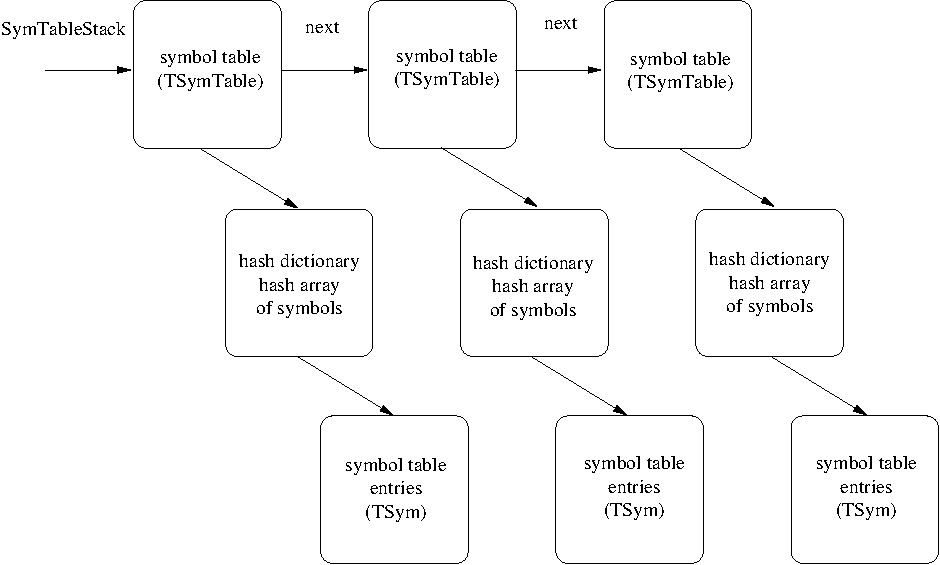
\includegraphics{arch4.pdf}
%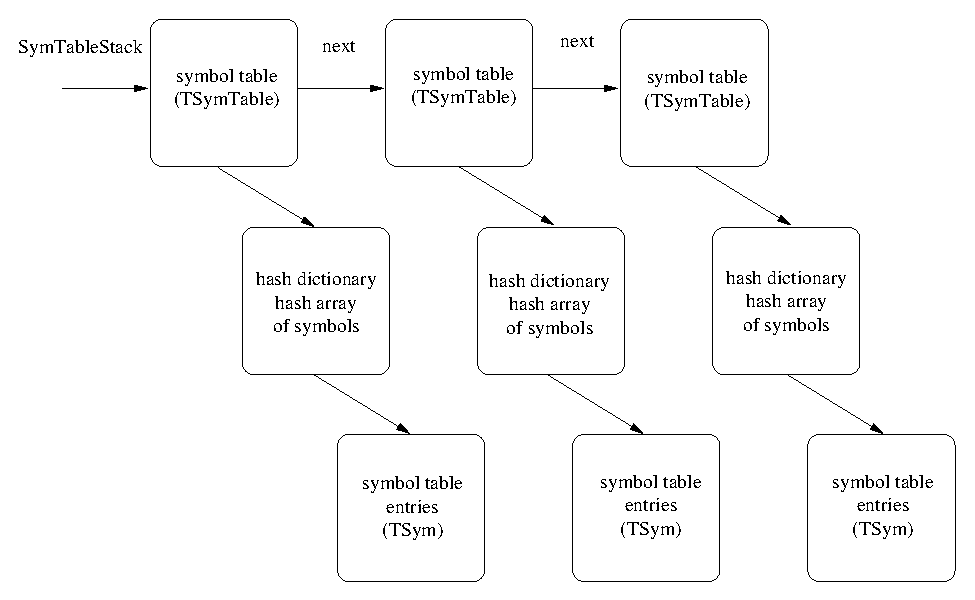
\epsfig{file=arch4.png,width=\textwidth}
\else
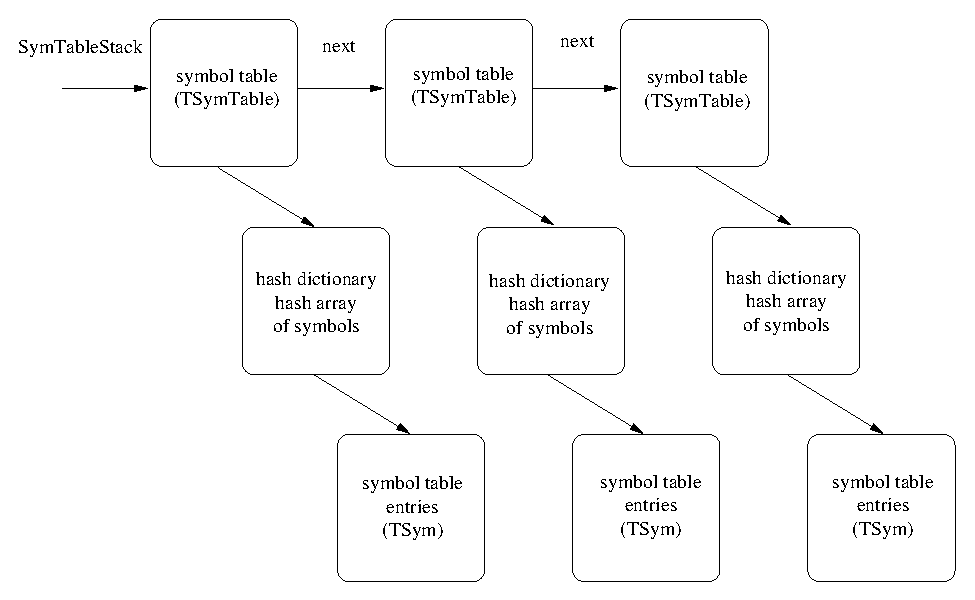
\includegraphics[width=6.29in,height=3.29in]{arch4.eps}
\fi
\label{fig4}
\caption{Interactions between symbol tables}
\end{figure}

As can be seen, the symbol table entries in the symbol table are done using
the fast hashing algorithm with a hash dictionary.

\subsection{The Symbol table object}
\label{subsec:mylabel3}

All symbol tables in the compiler are from this type of object, which
contains fields for the total size of the data in the symbol table, and
methods to read and write the symbol table into a stream. The start of the
linked list of active symbol tables is the \textbf{symtablestack} variable.

\begin{tabular*}{6.5in}{|l@{\extracolsep{\fill}}lp{6,5cm}|}
\hline
\textsf{TYPE} & & \\
\xspace \textsf{pSymTable} &= \^{} \textbf{TSymTable};&  \\
\xspace \textsf{TSymTable} &= \textbf{object} & \\
& \textsf{Name : pString;}& \\
& \textsf{DataSize : Longint;}&
	The total size of all the data in this symbol table (after the data has been aligned). Only valid for certain types of symbol tables. \\
& \textsf{DataAlignment : Longint;}& \\
& \textsf{SymIndex : pIndexArray;}& \\
& \textsf{DefIndex : pIndexArray;}&  \\
& \textsf{SymSearch : pDictionary;}& \\
& \textsf{Next : pSymtable;}&
	Points to the next symbol table in the linked list of active symbol tables. \\
& \textsf{DefOwner : pDef;}&
	The owner definition (only valid in the cases of objects and records, this points to the definition of that object or record). \\
& \textsf{Address{\_}Fixup : Longint}&  \\
& \textsf{UnitId : Word;}&  \\
& \textsf{SymTableLevel : Byte;}&  \\
& \textsf{SymTableType :TSymTableType;}&
	Indicates the type of this symbol table (\ref{fig2}). \\
&\textsf{end;}&  \\
\hline
\end{tabular*}

The type of possible symbol tables are shown in the following diagram:

\begin{longtable}{|l|p{10cm}|}
\hline
field	& Description \\
\hline
\endhead
\hline
\endfoot
TSymTableType& Description \\
\textsf{InvalidSymTable}&
	Default value when the symbol table is created and its type is not defined. Used for debugging purposes \\
\textsf{WithSymTable}&
	All symbols accessed in a with statement \\
\textsf{StaticSymTable}&  \\
\textsf{GlobalSymTable}&  \\
\textsf{UnitSymTable}&
	Linked list of units symbol used (all or unit?). The linked list is
	composed of \textsf{tunitsym} structures. \\
\textsf{ObjectSymTable}&  \\
\textsf{RecordSymTable}&
	Contains all symbols within a record statement \\
\textsf{MacroSymTable}&
	Holds all macros currently in scope. \\
\textsf{LocalSymTable}&
	Hold symbols for all local variables of a routine \\
\textsf{ParaSymTable}&
	Holds symbols for all parameters of a routine (the actual parameter declaration symbols) \\
\textsf{InlineParaSymTable}&
	Holds all parameter symbols for the current inline routine \\
\textsf{InlineLocalSymTable}&
	Holds all local symbols for the current inline routine \\
\textsf{Stt{\_}ExceptSymTable}&  \\
\textsf{StaticPPUSymTable}& 
\label{tab36}
\end{longtable}

\subsection{Inserting symbols into a symbol table}
\label{subsec:inserting}

To add a symbol into a specific symbol table, that's symbol table's
\textsf{Insert} method is called, which in turns call the
\textsf{Insert{\_}In{\_}Data} method of that symbol.
\textsf{Insert{\_}In{\_}Data}, depending on the symbol type, adjusts the
alignment and sizes of the data and actually creates the data entry in the
correct segment.

\begin{figure}
\ifpdf
%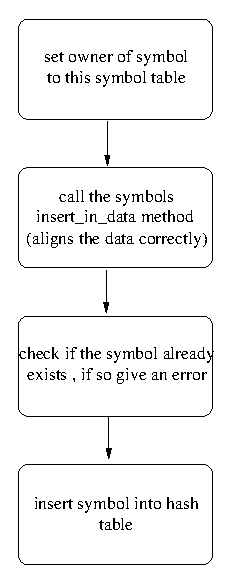
\epsfig{file=arch5.png,width=\textwidth}
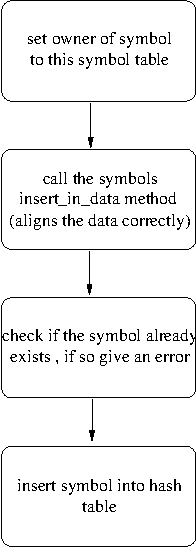
\includegraphics{arch5.pdf}
\else
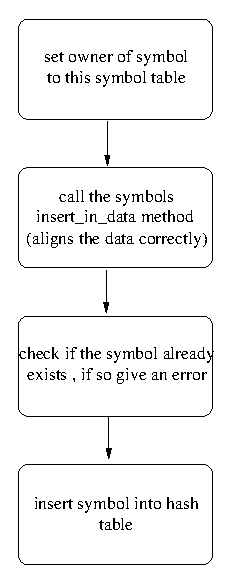
\includegraphics[width=1.51in,height=5.51in]{arch5.eps}
\fi
\label{fig5}
\caption{Inserting into the tree}
\end{figure}

\subsection{Symbol table interface}

\subsubsection{Routines}
\label{subsubsec:routinesable}

\begin{functionl}{Search{\_}a{\_}Symtable}{searchasymtable}
\Declaration
Function Search{\_}a{\_}Symtable(Const Symbol:String; \\
			SymTableType : TSymTableType):pSym;
\Description
Search for a symbol \textsf{Symbol} in a specified symbol table
\textsf{SymTableType}. Returns \textsf{NIL} if the symbol table is not
found, and also if the symbol cannot be found in the desired symbol table.
\end{functionl}

\begin{procedure}{GetSym}
\Declaration
Procedure GetSym(Const S : StringId; NotFoundError: Boolean);
\Description
Search all the active symbol tables for the symbol \textsf{s},setting the
global variable \textsf{SrSym} to the found symbol, or to \textsf{nil} if
the symbol was not found. \textsf{notfounderror} should be set to TRUE if
the routine must give out an error when the symbol is not found.
\end{procedure}

\begin{function}{GlobalDef}
\Declaration
Function GlobalDef(Const S : String) : pDef;
\Description
Returns a pointer to the definition of the fully qualified type symbol
\textsf{S}, or \textsf{NIL} if not found.
\Notes
It is fully qualified, in that the symbol \textsf{system.byte}, for example,
will be fully resolved to a unit and byte type component The symbol must
have a global scope, and it must be a type symbol, otherwise \textsf{NIL}
will be returned..
\end{function}

\subsubsection{Variables}
\label{subsubsec:variablesly}

\begin{variable}{SrSym}
\Declaration
Var SrSym : pSym;
\Description
This points to the symbol entry found, when calling \textsf{getsym}.
\end{variable}

\begin{variable}{SrSymTable}
\Declaration
Var SrSymTable : pSymTable;
\Description
This points to the symbol table of the symbol \seevar{SrSym} when calling
\seep{GetSym}.
\end{variable}

\section{Symbol entries}
\label{sec:mylabel3}

\subsection{Architecture}
\label{subsec:architecturees}

There are different possible types of symbols, each one having different
fields then the others. Each symbol type has a specific signature to
indicate what kind of entry it is. Each entry in the symbol table is
actually one of the symbol entries described in the following sections. The
relationship between a symbol entry, a type definition, and the type name
symbol entry is shown in figure \ref{fig6}.

\begin{figure}
\ifpdf
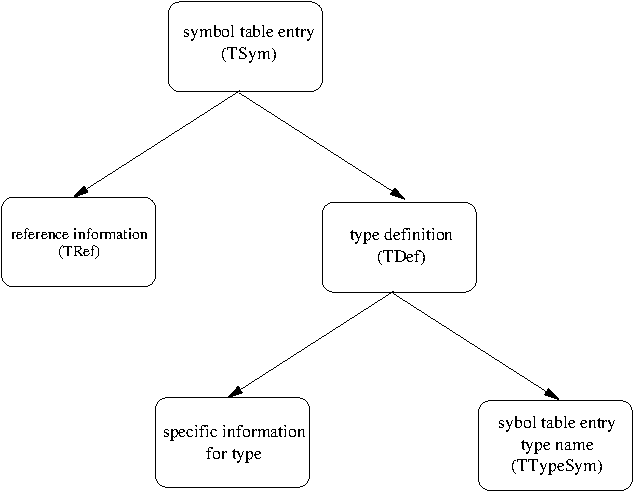
\includegraphics{arch6.pdf}
%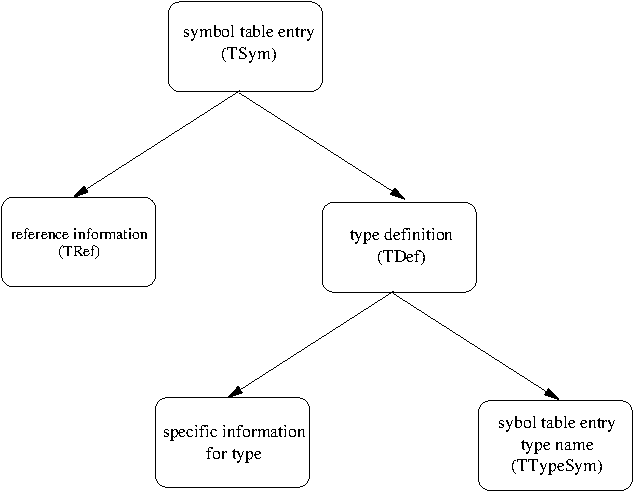
\epsfig{file=arch6.png,width=\textwidth}
\else
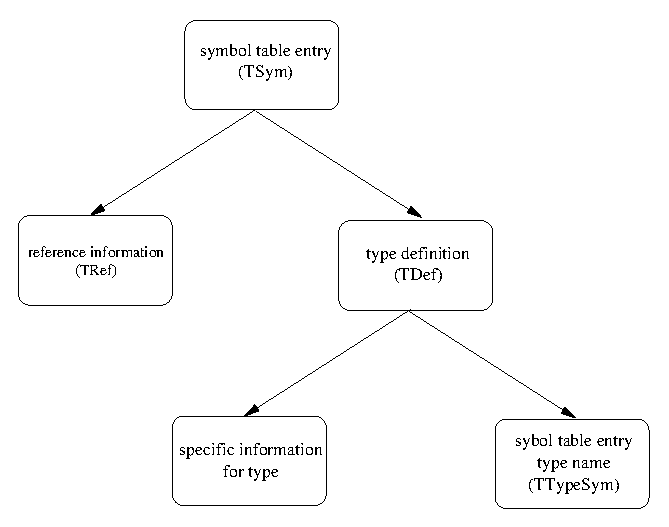
\includegraphics[width=5.51in,height=4.51in]{arch6.eps}
\fi
\label{fig6}
\caption{relation between symbol entry and type definition and name}
\end{figure}

\subsection{Symbol entry types}
\label{subsec:symbol}

\subsubsection{Base symbol type (TSym)}
\label{subsubsec:mylabel1}

All entries in the symbol table are derived from this base object which
contains information on the symbol type as well as information on the owner
of this symbol entry.

\begin{tabular*}{6.5in}{|l@{\extracolsep{\fill}}lp{9cm}|}
\hline
\textsf{TYPE} & &  \\
\xspace pSym = & \^{}  TSym; & \\
\xspace \textsf{TSym} = & \textbf{Object}(TSymTableEntry) & \\
& \textsf{SymOptions : TSymOptions;}& Indicate the access scope of the symbol \\
& \textsf{FileInfo : tFilePosInfo;}&  \\
& \textsf{Refs : Longint;}&
	Indicates how many times this label is refered in the parsed code (is only used with variable and assembler label symbols). \\
&\textsf{LastRef : pRef;}&  \\
&\textsf{DefRef : pRef;}&  \\
&\textsf{LastWritten : pRef;}& \\
&\textsf{RefCount : Longint;}& \\
&\textsf{Typ : tSymTyp;}& Indicates the symbol type (Cf. \ref{tab2}(. \\
&\textsf{IsStabWritten : Boolean;}& \\
&\textsf{end; }&\\
\hline 
\end{tabular*}

\begin{longtable}{|l|p{10cm}|}
\hline
TSymTyp	& Description \\
\hline
\endhead
\hline
\endfoot
\textsf{AbstractSym}&
	This is a special abstract symbol (this should never occur) \\
\textsf{VarSym}&
	This symbol is a variable declaration in the \textsf{var} section, or a \textsf{var} parameter. \\
\textsf{TypeSym}&
	This symbol is a type name \\
\textsf{ProcSym}&
	This symbol is a routine or method name \\
\textsf{UnitSym}&
	This symbol is a unit name \\
\textsf{\textit{ProgramSym}}&
	\textit{This symbol is the main program name} \\
\textsf{ConstSym}&
	This symbol is a constant \\
\textsf{EnumSym}&
	This symbol is an enumeration symbol (an element in an enumeration) \\
\textsf{TypedConstSym}&
	This symbol is pre-initialized variable (pascal typed constant) \\
\textsf{ErrorSym}&
	This symbol is created for error generation \\
\textsf{SysSym}&
	This symbol represents an inlined system unit routine \\
\textsf{LabelSym}&
	This symbol represents a label in a \textsf{label} pascal declaration \\
\textsf{AbsoluteSym}&
	This symbol represents an the symbol following an \textsf{absolute} variable declaration \\
\textsf{PropertySym}&
	This symbol is a property name \\
\textsf{FuncRetSym}&
	This symbol is the name of the return value for functions \\
\textsf{MacroSym}&
	This symbol is a macro symbol (just like {\#}define in C)
\end{longtable}

\subsubsection{label symbol (TLabelSym)}
\label{subsubsec:label}

The label symbol table entry is only created when a pascal label is declared
via the label keyword. The object has the following fields which are
available for use publicly:

\begin{tabular*}{6.5in}{|l@{\extracolsep{\fill}}lp{9cm}|}
\hline
\textsf{TYPE} & &  \\
\xspace pLabelSym = & \^{}  TLabelSym; & \\
\xspace \textsf{TLabelSym} = & \textbf{Object}(TSym) & \\
& \textsf{Used : Boolean}&
	Set to TRUE if this pascal label is used using a \textsf{goto} or in an assembler statement \\
& \textsf{Defined: Boolean}&
	Set to TRUE if this label has been declared \\
& \textsf{Lab : pAsmLabel}&
	Points to the actual assembler label structure which will be emitted by the code generator \\
& \textsf{Code : Pointer}&  \\
& \textsf{end;}&  \\
\hline
\end{tabular*}

\subsubsection{unit symbol (TUnitSym)}
\label{subsubsec:mylabel2}

The unit symbol is created and added to the symbol table each time that the
uses clause is parsed and a unit name is found, it is also used when
compiling a unit, with the first entry in that symbol table being the unit
name being compiled. The unit symbol entry is actual part of a linked list
which is used in the unit symbol table.

\begin{tabular*}{6.5in}{|l@{\extracolsep{\fill}}lp{7cm}|}
\hline
\textsf{TYPE} & & \\
\xspace pUnitSym = & \^{}  TUnitSym; & \\
\xspace \textsf{TUnitSym} = & \textbf{Object}(TSym) & \\
& \textsf{UnitSymTable:pUnitSymTable}&
	Pointer to the global symbol table for that unit, containing entries for each public? symbol in that unit \\
& \textsf{PrevSym : pUnitSym}&
	Pointer to previous entry in the linked list \\
& \textsf{end;}&  \\
\hline
\end{tabular*}

\subsubsection{macro symbol (TMacroSym)}
\label{subsubsec:macro}

The macro synbols are used in the preprocessor for conditional compilation
statements. There is one such entry created for each {\$}define directive,
it contains the value of the define (stored as a string).

\begin{tabular*}{6.5in}{|l@{\extracolsep{\fill}}lp{6cm}|}
\hline
\textsf{TYPE}& & \\
\xspace pMacroSym = & \^{}  TMacroSym; & \\
\xspace \textsf{TMacroSym} = & \textbf{Object}(TSym) & \\
& \textsf{Defined : Boolean;}&
	TRUE if the symbol has been defined with a \textsf{{\$}define}
	directive, or false if it has been undefined with a
	\textsf{{\$}undef} directive \\
& \textsf{Defined{\_}At{\_}Startup : Boolean;}&
	TRUE if the symbol is a system wide define \\
& \textsf{Is{\_}Used: Boolean;}&
	TRUE if the define has been used such as in a \textsf{{\$}ifdef}
	directive. \\
& \textsf{BufText : pChar;}&
	The actual string text of the define \\
& \textsf{BufLength : Longint;}&
	The actual string length of the define \\
& \textsf{end;}&  \\
\hline
\end{tabular*}

\subsubsection{error symbol (TErrorSym)}
\label{subsubsec:error}

This symbol is actually an empty symbol table entry. When the parser
encounters an error when parsing a symbol, instead of putting nothing in the
symbol table, it puts this symbol entry. This avoids illegal memory accesses
later in parsing.

\subsubsection{procedure symbol (TProcSym)}
\label{subsubsec:procedure}

The procedure symbol is created each time a routine is defined in the code.
This can be either a forward definition or the actual implementation of the
routine. After creation, the symbol is added into the appropriate symbol
table stack.

\begin{tabular*}{6.5in}{|l@{\extracolsep{\fill}}lp{8cm}|}
\hline
\textsf{TYPE}& & \\
\xspace pProcSym = & \^{}  TProcSym; & \\
\xspace \textsf{TProcSym} = & \textbf{Object}(TSym) & \\
& \textsf{Is{\_}Global : Boolean}&
	Set if the routine is exported by the unit \\
& \textsf{Definition : pProcDef}&
	Procedure definition, including parameter information and return
	values \\
& \textsf{end;}&  \\
\hline
\end{tabular*}

\subsubsection{type symbol (TTypeSym)}
\label{subsubsec:mylabel3}

The type symbol is created each time a new type declaration is done, the
current symbol table stack is then inserted with this symbol. Furthermore,
each time the compiler compiles a module, the default base types are
initialized and added into the symbol table (\textbf{psystem.pas}) The type
symbol contains the name of a type, as well as a pointer to its type
definition.

\begin{tabular*}{6.5in}{|l@{\extracolsep{\fill}}lp{9cm}|}
\hline
\textsf{TYPE}& &  \\
\xspace pTypeSym = & \^{}  TTypeSym; & \\
\xspace \textsf{TTypeSym} = & \textbf{Object}(TSym) & \\
& \textsf{ResType : TType}&
	Contains base type information as well as the type definition \\
& \textsf{end;}&  \\
\hline
\end{tabular*}

\subsubsection{variable symbol (TVarSym)}
\label{subsubsec:variable}

Variable declarations, as well as parameters which are passed onto routines
are declared as variable symbol types. Access information, as well as type
information and optimization information are stored in this symbol type.

\begin{tabular*}{6.5in}{|l@{\extracolsep{\fill}}lp{8.5cm}|}
\hline
\textsf{TYPE}& & \\
\xspace pVarSym = & \^{}  TVarSym; & \\
\xspace \textsf{TVarSym} = & \textbf{Object}(TSym) & \\
& \textsf{Reg: TRegister;}&
	If the value is a register variable, the \textsf{reg} field will be
	different then R{\_}NO \\
& \textsf{VarSpez : TVarSpez;}&
	Indicates the variable type (parameters only) (Cf. \ref{tab4}). \\
& \textsf{Address : Longint;}&
	In the case where the variable is a routine parameter, this
	indicates the positive offset from the \textsf{frame{\_}pointer }to
	access this variable. In the case of a local variable, this field
	indicates the negative offset from the \textsf{frame{\_}pointer}. to
	access this variable. \\
& \textsf{LocalVarSym : pVarSym;}&  \\
& \textsf{VarType : TType;}&
	Contains base type information as well as the type definition \\
& \textsf{VarOptions : TVarOptions;}&
	Flags for this variable (Cf. \ref{tab3}) \\
& \textsf{VarState : TVarState}&
	Indicates the state of the variable, if it's used or declared \\
& \textsf{end;}&  \\
\hline
\end{tabular*}

\begin{longtable}{|l|p{10cm}|}
\hline
TVarOptions & Description \\
\hline
\endhead
\hline
\endfoot
\textsf{vo{\_}Regable}&
	The variable can be put into a hardware general purpose register \\
\textsf{vo{\_}Is{\_}C{\_}Var}&
	The variable is imported from a C module \\
\textsf{vo{\_}Is{\_}External}&
	The variable is declared external \\
\textsf{vo{\_}Is{\_}Dll{\_}Var}&
	The variable is a shared library variable \\
\textsf{vo{\_}Is{\_}Thread{\_}Var}&
	The variable is declared as being thread safe \\
\textsf{vo{\_}FpuRegable}&
	The variable can be put into a hardware floating point register \\
\textsf{vo{\_}Is{\_}Local{\_}Copy}&  \\
\textsf{\textit{vo{\_}Is{\_}Const}}&
	\textit{unused and useless} \\
\textsf{vo{\_}Is{\_}Exported}&
	The variable is declared as exported in a dynamic link library 
\end{longtable}

\begin{longtable}{|l|p{10cm}|}
\hline
TVarSpez & Description \\
\hline
\endhead
\hline
\endfoot
\textsf{vs{\_}Value}&
	This is a value parameter \\
\textsf{vs{\_}Const}&
	This is a constant parameter, property or array \\
\textsf{vs{\_}Var}&
	This is a variable parameter
\end{longtable}

\subsubsection{property symbol}
\label{subsubsec:property}

\subsubsection{return value of function symbol}
\label{subsubsec:return}

\subsubsection{absolute declared variable}
\label{subsubsec:absolute}

\subsubsection{typed constant symbol}
\label{subsubsec:typed}

\subsubsection{constant symbol}
\label{subsubsec:constant}

\subsubsection{enumeration symbol}
\label{subsubsec:enumeration}

\subsubsection{program symbol}
\label{subsubsec:program}

\subsubsection{sys symbol}
\label{subsubsec:mylabel4}

\subsection{Symbol interface}
\label{subsec:mylabel5}

\section{Type information}
\label{sec:mylabel4}

\subsection{Architecture}
\label{subsec:architecturetionolbo}

A type declaration , which is the basis for the symbol table, since
inherently everything comes down to a type after parsing is a special
structure with two principal fields, which point to a symbol table entry
which is the type name, and the actual definition which gives the
information on other symbols in the type, the size of the type and other
such information.

\begin{tabular*}{6.5in}{|l@{\extracolsep{\fill}}lp{9cm}|}
\hline
\textsf{TYPE} & &  \\
\xspace \textsf{TType} = & \textbf{Object} & \\
&\textsf{Sym : pSym;}&
	Points to the symbol table of this type \\
& \textsf{Def : pDef;}&
	Points to the actual definition of this type \\
&\textsf{end;}&   \\
\hline
\end{tabular*}

\begin{figure}
\ifpdf
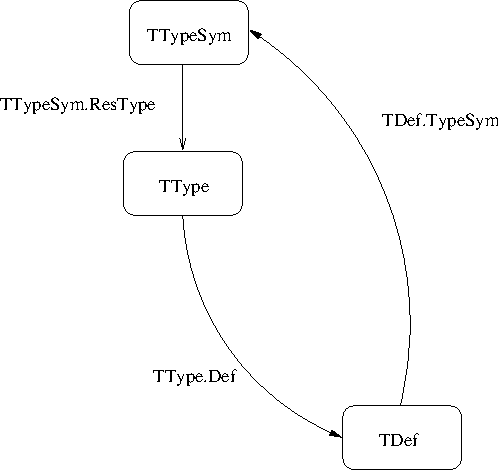
\includegraphics{arch7.pdf}
%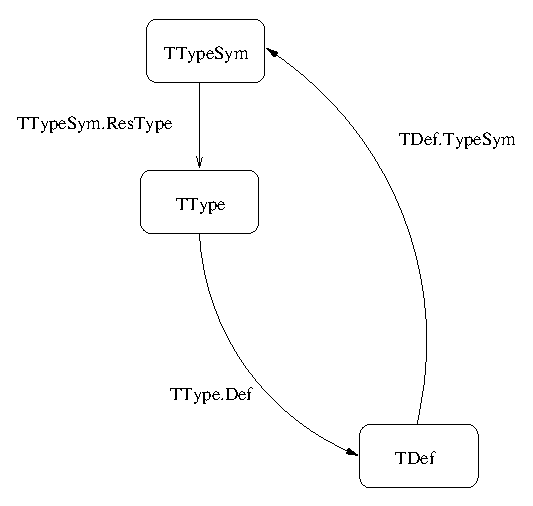
\epsfig{file=arch7.png,width=\textwidth}
\else
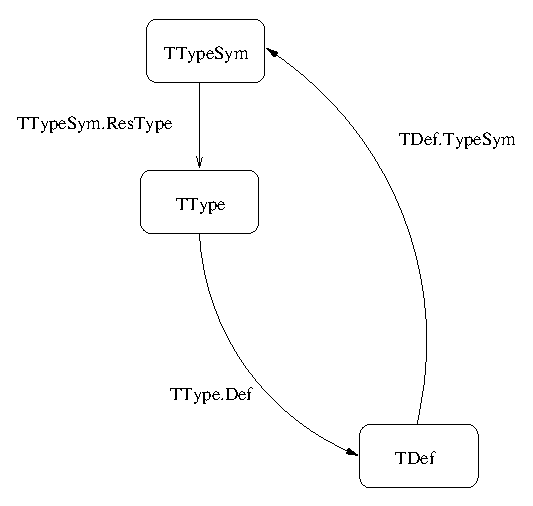
\includegraphics[width=4.39in,height=3.56in]{arch7.eps}
\fi
\caption{Type symbol and definition relations}
\label{fig7}

\end{figure}

\subsection{Definition types}

Definitions represent the type information for all possible symbols which
can be encountered by the parser. The definition types are associated with
symbols in the symbol table, and are used by the parsing process (among
other things) to perform type checking.

The current possible definition types are enumerated in \textsf{TDefType}
and can have one of the following symbolic values:

\begin{longtable}{|l|p{10cm}|}
\hline
deftype of TDef object	& Description \\
\hline
\endhead
\hline
\endfoot
\textsf{AbstractDef}	&  \\
\textsf{ArrayDef}	& array type definition \\
\textsf{RecordDef}	& record type definition \\
\textsf{PointerDef}	& pointer type definition \\
\textsf{OrdDef}		& ordinal (numeric value) type definition \\
\textsf{StringDef}	& string type definition \\
\textsf{EnumDef}	& enumeration type definition \\
\textsf{ProcDef}	& procedure type definition \\
\textsf{ObjectDef}	& object or class type definition \\
\textsf{ErrorDef}	& error definition (empty, used for error recovery) \\
\textsf{FileDef}	& file type definition \\
\textsf{FormalDef}	&  \\
\textsf{SetDef}		& set type definition \\
\textsf{ProcVarDef}	& procedure variable type definition \\
\textsf{FloatDef}	& floating point type definition \\
\textsf{ClassrefDef}	&  \\
\textsf{ForwardDef}	&  \\
\end{longtable}

\subsubsection{base definition (TDef)}
\label{subsubsec:mylabel5}

All type definitions are based on this object. Therefore all derived object
all posess the fields in this object in addition to their own private
fields.

\begin{tabular*}{6.5in}{|l@{\extracolsep{\fill}}lp{7cm}|}
\hline
\textsf{TYPE} & & \\
\xspace pDef = & \^{}  TDef; & \\
\xspace \textsf{TDef} = & \textbf{Object}(TSymTableEntry) & \\
&\textsf{TypeSym : pTypeSym;}&
	Pointer to symbol table entry for this type definition \\
&\textsf{InitTable{\_}Label : pAsmLabel;}&
	Label to initialization information (required for some complex types) \\
&\textsf{Rtti{\_}Label : pAsmLabel;}&
	Label to the runtime type information. \\
&\textsf{NextGlobal : pDef;}&  \\
&\textsf{PreviousGlobal : pDef;}&  \\
&\textsf{SaveSize : Longint;}&
	Size in bytes of the data definition \\
&\textsf{DefType : tDefType;}&
	Indicates the definition type (see \ref{tab5}). \\
&\textsf{Has{\_}InitTable : Boolean;}&  \\
&\textsf{Has{\_}Rtti : Boolean;}&  \\
&\textsf{Is{\_}Def{\_}Stab{\_}Written : TDefStabStatus}&
	Can be one of the following states : (\textsf{Not{\_}Written,
	written, Being{\_}Written}) which indicates if the debug information
	for this type has been defined or not. \\
&\textsf{GlobalNb : Longint;}&
	Internal debug information type signature (each definition has a
	numeric signature). \\
&\textsf{end;}&  \\
\hline
\end{tabular*}

\subsubsection{file definition (TFileDef)}
\label{subsubsec:mylabel6}

The file definition can occur in only some rare instances, when a
\textsf{file of }\textsf{\textit{type}} is parsed, a file definition of that
type will be created. Furthermore, internally, a definition for a
\textbf{Text} file type and \textbf{untyped} File type are created when the
system unit is loaded. These types are always defined when compiling any
unit or program.

\begin{tabular*}{6.5in}{|l@{\extracolsep{\fill}}lp{8.5cm}|}
\hline
\textsf{TYPE}& &   \\
\xspace pFileDef = & \^{}  TFileDef; & \\
\xspace \textsf{TFileDef} = & \textbf{Object}(TDef) & \\
&\textsf{FileTyp : TFileTyp;}&
	Indicates what type of file definition it is (\textsf{text},
	\textsf{untyped} or \textsf{typed}). \\
&\textsf{TypedFileType : TType;}&
	In the case of a typed file definition, definition of the type of
	the file \\
&\textsf{end;}&  \\
\hline
\end{tabular*}

\subsubsection{formal definition (TFormalDef)}
\label{subsubsec:formal}

\subsubsection{forward definition (TForwardDef)}
\label{subsubsec:forward}

The forward definition is created, when a type is declared before an actual
definition exists. This is the case, when, for example \textsf{type
pmyobject = \ tmyobject}, while \textsf{tmyobject} has yet to be defined.

\begin{tabular*}{6.5in}{|l@{\extracolsep{\fill}}lp{6.5cm}|}
\hline
\textsf{TYPE} & &  \\
\xspace pForwardDef = & \^{}  TForwardDef; & \\
\xspace \textsf{TForwardDef} = & \textbf{Object}(TDef) & \\
&\textsf{toSymName : String;}&
	The symbol name for this forward declaration (the actual real
	definition does not exist yet) \\
&\textsf{ForwardPos : TFilePosInfo;}&
	Indicates file position where this forward definition was declared. \\
&\textsf{end;}&  \\
\hline
\end{tabular*}

\subsubsection{error definition (TErrorDef)}
\label{subsubsec:mylabel7}

This definition is actually an empty definition entry. When the parser
encounters an error when parsing a definition instead of putting nothing in
the type for a symbol, it puts this entry. This avoids illegal memory
accesses later in parsing.

\subsubsection{pointer definition (TPointerDef)}
\label{subsubsec:pointer}

The pointer definition is used for distinguishing between different types of
pointers in the compiler, and are created at each \textsf{\ typename}
parsing construct found.

\begin{tabular*}{6.5in}{|l@{\extracolsep{\fill}}lp{9cm}|}
\hline
\textsf{TYPE} & & \\
\xspace pPointerDef = & \^{}  TPointerDef; & \\
\xspace \textsf{TPointerDef} = & \textbf{Object}(TDef) & \\
&\textsf{Is{\_}Far : Boolean;}&
	Used to indicate if this is a far pointer or not (this flag is
	cpu-specific) \\
&\textsf{PointerType : TType;}&
	This indicates to what type definition this pointer points to. \\
&\textsf{end;}&  \\
\hline
\end{tabular*}

\subsubsection{object definition (TObjectDef)}
\label{subsubsec:object}

The object definition is created each time an object declaration is found in
the type declaration section.

\begin{tabular*}{6.5in}{|l@{\extracolsep{\fill}}lp{6cm}|}
\hline
\textsf{TYPE}& & \\
\xspace pObjectDef = & \^{}  TObjectDef; & \\
\xspace \textsf{TObjectDef} = & \textbf{Object}(TDef) & \\
&\textsf{ChildOf : pObjectDef;}&
	This is a pointer to the parent object definition. It is set to nil,
	if this object definition has no parent. \\
&\textsf{ObjName : pString;}&
	This is the object name \\
&\textsf{SymTable : pSymTable;}&
	This is a pointer to the symbol table entries within this object. \\
&\textsf{PbjectOptions : TObjectOptions;}&
	The options for this object, see the following table for the
	possible options for the object. \\
&\textsf{VMT{\_}Offset : Longint;}&
	This is the offset from the start of the object image in memory
	where the virtual method table is located. \\
&\textsf{Writing{\_}Class{\_}Record{\_}Stab : Boolean;}&  \\
&\textsf{end;}&  \\
\hline
\end{tabular*}


\begin{longtable}{|l|p{10cm}|}
\hline
Object Options(TObjectOptions) & Description \\
\hline
\endhead
\hline
\endfoot
\textsf{oo{\_}Is{\_}Class}&
	This is a delphi styled class declaration, and not a Turbo Pascal
	object. \\
\textsf{oo{\_}Is{\_}Forward}&
	This flag is set to indicate that the object has been declared in a
	type section, but there is no implementation yet. \\
\textsf{oo{\_}Has{\_}Virtual}&
	This object / class contains virtual methods \\
\textsf{oo{\_}Has{\_}Private}&
	This object / class contains private fields or methods \\
\textsf{oo{\_}Has{\_}Protected}&
	This object / class contains protected fields or methods \\
\textsf{oo{\_}Has{\_}Constructor}&
	This object / class has a constructor method \\
\textsf{oo{\_}Has{\_}Destructor}&
	This object / class has a destructor method \\
\textsf{oo{\_}Has{\_}VMT}&
	This object / class has a virtual method table \\
\textsf{oo{\_}Has{\_}Msgstr}&
	This object / class contains one or more message handlers  \\
\textsf{oo{\_}Has{\_}Msgint}&
	This object / class contains one or more message handlers  \\
\textsf{oo{\_}Has{\_}Abstract}&
	This object / class contains one or more abstract methods \\
\textsf{oo{\_}Can{\_}Have{\_}Published}&
	the class has runtime type information, i.e. you can publish
	properties \\
\textsf{oo{\_}CPP{\_}Class}&
	the object/class uses an C++ compatible class layout \\
\textsf{oo{\_}Interface}&
	this class is a delphi styled interface
\end{longtable}

\subsubsection{class reference definition (TClassRefDef)}
\label{subsubsec:class}

\subsubsection{array definition (TArrayDef)}
\label{subsubsec:array}

This definition is created when an array type declaration is parsed. It
contains all the information necessary for array type checking and code
generation.

\begin{tabular*}{6.5in}{|l@{\extracolsep{\fill}}lp{8.4cm}|}
\hline
\textsf{TYPE}& & \\
\xspace pArrayDef = & \^{}  TArrayDef; & \\
\xspace \textsf{TArrayDef} = & \textbf{Object}(TDef) & \\
&\textsf{IsVariant : Boolean;}&  \\
&\textsf{IsConstructor : Boolean;}&  \\
&\textsf{RangeNr: Longint;}&
	Label number associated with the index values when range checking is
	on \\
&\textsf{LowRange : Longint;}&
	The lower index range of the array definition \\
&\textsf{HighRange : Longint;}&
	The higher index range of the array definition \\
&\textsf{ElementType : TType;}&
	The type information for the elements of the array \\
&\textsf{RangeType : TType;}&
	The type information for the index ranges of the array \\
&\textsf{IsArrayofConst : Boolean;}&  \\
&\textsf{end;}& \\
\hline
\end{tabular*}

\subsubsection{record definition (TRecordDef)}
\label{subsubsec:record}

The record definition entry is created each time a record type declaration
is parsed. It contains the symbol table to the elements in the record.

\begin{tabular*}{6.5in}{|l@{\extracolsep{\fill}}lp{8.7cm}|}
\hline
\textsf{TYPE} & & \\
\xspace pRecordDef = & \^{}  TRecordDef; & \\
\xspace \textsf{TRecordDef} = & \textbf{Object}(TDef) & \\
&\textsf{SymTable : PSymTable;}&
	This is a pointer to the symbol table entries within this record. \\
&\textsf{end;}&  \\
\hline
\end{tabular*}

\subsubsection{ordinal definition (TOrdDef)}
\label{subsubsec:ordinal}

This type definition is the one used for all ordinal values such as char,
bytes and other numeric integer type values. Some of the predefined type
definitions are automatically created and loaded when the compiler starts.
Others are created at compile time, when declared.

\begin{tabular*}{6.5in}{|l@{\extracolsep{\fill}}lp{9cm}|}
\hline
\textsf{TYPE} & &  \\
\xspace pOrdDef = & \^{}  TOrdDef; & \\
\xspace \textsf{TOrdDef} = & \textbf{Object}(TDef) & \\
&\textsf{Low : Longint;}&
	The minimum value of this ordinal type \\
&\textsf{High : Longint;}&
	The maximum value of this ordinal type \\
&\textsf{Typ : TBaseType;}&
	The type of ordinal value (cf. \ref{fig3}) \\
&\textsf{end;}&  \\
\hline
\end{tabular*}

\begin{longtable}{|l|p{10cm}|}
\hline
Base ordinal type (TBaseType) & Description \\
\hline
\endhead
\hline
\endfoot
\textsf{uauto} & user defined ordinal type definition \\
\textsf{uvoid} & Represents a void return value or node \\
\textsf{uchar} & ASCII character (1 byte) \\
\textsf{u8bit} & unsigned 8-bit value \\
\textsf{u16bit}& unsigned 16-bit value \\
\textsf{u32bit}& unsigned 32-bit value \\
\textsf{s16bit}& signed 16-bit value \\
\textsf{s32bit}& signed 32-bit value \\
\textsf{bool8bit}& boolean 8-bit value \\
\textsf{bool16bit}& boolean 16-bit value \\
\textsf{bool32bit}& boolean 32-bit value \\
\textsf{\textit{u64bit}}&
	\textit{unsigned 64-bit value (not fully supported/tested)} \\
\textsf{s64bit}& signed 64-bit value \\\textsf{\textit{uwidechar}}&
	\textit{Currently not supported and unused} \\
\end{longtable}

\subsubsection{float definition (TFloatDef)}
\label{subsubsec:float}

This type definition is the one used for all floating point values such as
SINGLE, DOUBLE. Some of the predefined type definitions are automatically
created and loaded when the compiler starts.

\begin{tabular*}{6.5in}{|l@{\extracolsep{\fill}}lp{9cm}|}
\hline
\textsf{TYPE} & &  \\
\xspace pFloatDef = & \^{}  TFloatDef; & \\
\xspace \textsf{TFloatDef} = & \textbf{Object}(TDef) & \\
&\textsf{Typ : TFloatType;}&
	The type of floating point value (cf. \ref{tab6}). \\
&\textsf{end;}&  \\
\hline
\end{tabular*}

\begin{longtable}{|l|p{10cm}|}
\hline
Base floating point type (TFloatType) & Description \\
\hline
\endhead
\hline
\endfoot
\textsf{s32real}& IEEE Single precision floating point value \\
\textsf{s64real}& IEEE Double precision floating point value \\
\textsf{s80real}&
		Extended precision floating point value (cpu-specific,
		usually maps to double) \\
\textsf{s64comp}& 63-bit signed value, using 1 bit for sign indication \\
\textsf{\textit{f16bit}}& \textit{Unsupported} \\
\textsf{\textit{f32bit}}& \textit{Unsupported} \\
\end{longtable}

\subsubsection{abstract procedure definition (tabstractprocdef)}
\label{subsubsec:abstract}

This is the base of all routine type definitions. This object is abstract,
and is not directly used in a useful way. The derived object of this object
are used for the actual parsing process.

\begin{tabular*}{6.5in}{|l@{\extracolsep{\fill}}lp{5.5cm}|}
\hline
\textsf{TYPE}& & \\
\xspace pAbstractProcDef = & \^{}  TAbstractProcDef; & \\
\xspace \textsf{TAbstractProcDef} = & \textbf{Object}(TDef) & \\
&\textsf{SymtableLevel : byte;}&  \\
&\textsf{Fpu{\_}Used : Byte;}&
	Number of floating point registers used in this routine  \\
&\textsf{RetType : TType;}&
	Type information for the return value \par (uvoid if it returns nothing) \\
&\textsf{ProcTypeOption : TProcTypeOption;} &
	Indicates the type of routine it is (cf \ref{tab7}). \\
&\textsf{ProcCallOptions : TProcCallOptions;} &
	Indicates the calling convention of the routine (cf. \ref{tab8}). \\
&\textsf{ProcOptions : TProcOptions;}&
	Indicates general procedure options.  \par (cf. \ref{tab9}). \\
&\textsf{Para : pLinkedList;}&
	This is a linked list of parameters (pparaitem list) \\
&\textsf{end;}&  \\
\hline
\end{tabular*}

\begin{longtable}{|l|p{10cm}|}
\hline
Procedure options  \par (TProcTypeOption)& Description \\
\hline
\endhead
\hline
\endfoot
\textsf{poType{\_}ProgInit}&
	Routine is the program entry point (defined as `\textsf{main}' in
	the compiler). \\
\textsf{poType{\_}UnitInit}&
	Routine is the unit initialization code \par (defined as
	unitname\textsf{{\_}init} in the compiler \\
\textsf{poType{\_}UnitFinalize}&
	Routine is the unit exit code \par (defined as
	unitname\textsf{{\_}finalize} in the compiler) \\
\textsf{poType{\_}Constructor}&
	Routine is an object or class constructor \\
\textsf{poType{\_}Destructor}&
	Routine is an object or class destructor \\
\textsf{poType{\_}Operator}&
	Procedure is an operator \\
\end{longtable}

\begin{longtable}{|l|p{10cm}|}
\hline
call options \par (TProcCallOptions) & Description \\
\hline
\endhead
\hline
\endfoot
\textsf{poCall{\_}ClearStack}&
	The routine caller clears the stack upon return \\
\textsf{poCall{\_}LeftRight}&
	Send parameters to routine from left to right \\
\textsf{poCall{\_}Cdecl}&
	Passing parameters is done using the GCC alignment scheme, passing
	parameter values is directly copied into the stack space \\
\textsf{\textit{poCall{\_}Register}}&
	\textit{unused (Send parameters via registers)} \\
\textsf{poCall{\_}StdCall}&
	Passing parameters is done using GCC alignment scheme \\
\textsf{\textit{poCall{\_}SafeCall}}&
	\textit{unused} \\
\textsf{\textit{poCall{\_}PalmOsSyscall}}&
	\textit{unused} \\
\textsf{\textit{poCall{\_}System}}&
	\textit{unused} \\
\textsf{poCall{\_}Inline}&
	Routine is an inline assembler macro (not a true call) \\
\textsf{poCall{\_}InternProc}&
	System unit code generator helper routine \\
\textsf{poCall{\_}InternConst}&
	System unit code generator helper macro routine \\
\end{longtable}

\begin{longtable}{|l|p{10cm}|}
\hline
routine options (TProcOptions) & Description \\
\hline
\endhead
\hline
\endfoot
\textsf{po{\_}ClassMethod}   & This is a class method \\
\textsf{po{\_}VirtualMethod }& This is a virtual method \\
\textsf{po{\_}AbstractMethod}& This is an abstract method \\
\textsf{po{\_}StaticMethod}  & This is a static method \\
\textsf{po{\_}OverridingMethod}&
	This is an overriden method (with po{\_}virtual flag usually) \\
\textsf{po{\_}MethodPointer}&
	This is a method pointer (not a normal routine pointer) \\
\textsf{po{\_}ContainsSelf}&
	self is passed explicitly as a parameter to the method \\
\textsf{po{\_}Interrupt}&
	This routine is an interrupt handler \\
\textsf{po{\_}IOCheck}&
	IO checking should be done after a call to the procedure \\
\textsf{po{\_}Assembler}&
	The routine is in assembler \\
\textsf{po{\_}MsgStr}&
	method for string message handling \\
\textsf{po{\_}MsgInt}&
	method for int message handling \\
\textsf{po{\_}Exports}&
	Routine has export directive  \\
\textsf{po{\_}External}&
	Routine is external (in other object or lib) \\
\textsf{po{\_}SaveStdRegs}&
	Routine entry should save all registers used by GCC \\
\textsf{po{\_}SaveRegisters}&
	Routine entry should save all registers \\
\textsf{po{\_}OverLoad}&
	Routine is declared as being overloaded \\
\end{longtable}

\subsubsection{procedural variable definition (TProcVarDef)}
\label{subsubsec:procedural}

This definition is created when a procedure variable type is declared. It
gives information on the type of a procedure, and is used when assigning and
directly calling a routine through a pointer.

\begin{tabular*}{6.5in}{|l@{\extracolsep{\fill}}lp{7.8cm}|}
\hline
\textsf{TYPE} & &  \\
\xspace pProcVarDef = & \^{}  TProcVarDef; & \\
\xspace \textsf{TProcVarDef} = & \textbf{Object}(TAbstractProcDef) & \\
& \textsf{end;}&\\
\hline
\end{tabular*}

\subsubsection{procedure definition (TProcDef)}
\label{subsubsec:mylabel8}

When a procedure head is parsed, the definition of the routine is created.
Thereafter, other fields containing information on the definition of the
routine are populated as required.

\begin{tabular*}{6.5in}{|l@{\extracolsep{\fill}}lp{7.8cm}|}
\hline
\textsf{TYPE} & &  \\
\xspace pProcDef = & \^{}  TProcDef; & \\
\xspace \textsf{TProcDef} = & \textbf{Object}(TAbstractProcDef) & \\
&\textsf{ForwardDef : Boolean;}& TRUE if this is a forward definition \\
&\textsf{InterfaceDef: Boolean;}&  \\
&\textsf{ExtNumber : Longint;}&  \\
&\textsf{MessageInf : TMessageInf;}&  \\
&\textsf{NextOverloaded : pProcDef;}&  \\
&\textsf{FileInfo : TFilePosInfo;}&
	Position in source code for the declaration of this routine. Used
	for error management. \\
&\textsf{Localst : pSymTable;}& The local variables symbol table \\
&\textsf{Parast: pSymTable;}& The parameter symbol table \\
&\textsf{ProcSym : pProcSym;}& Points to owner of this definition \\
&\textsf{LastRef : pRef;}&  \\
&\textsf{DefRef: pRef;}&  \\
&\textsf{CrossRef : pRef;}&  \\
&\textsf{LastWritten : pRef;}&  \\
&\textsf{RefCount : Longint;}&  \\
&\textsf{{\_}Class : ProbjectDef;}&  \\
&\textsf{Code : Pointer;}&
	The actual code for the routine (only for inlined routines) \\
&\textsf{UsedRegisters : TRegisterSet;}&
	The set of registers used in this routine \\
&\textsf{HasForward : Boolean;}&  \\
&\textsf{Count: Boolean;}&  \\
&\textsf{Is{\_}Used : Boolean;}&  \\
&\textsf{end;}&  \\
\hline
\end{tabular*}

\subsubsection{string definition (TStringDef)}
\label{subsubsec:string}

This definition represents all string types as well as derived types. Some
of the default string type definitions are loaded when the compiler starts
up. Others are created at compile time as they are declared with a specific
length type.

\begin{tabular*}{6.5in}{|l@{\extracolsep{\fill}}lp{9cm}|}
\hline
\textsf{TYPE}& & \\
\xspace pStringDef = & \^{}  TStringDef; & \\
\xspace \textsf{TStringDef} = & \textbf{Object}(TDef) & \\
&\textsf{String{\_}Typ : TStringType;}&
	Indicates the string type definition (cf. \ref{tab10}) \\
&\textsf{Len : Longint;}&
	This is the maximum length which can have the string \\
&\textsf{end;}& \\
\hline
\end{tabular*}

\begin{longtable}{|l|p{10cm}|}
\hline
String type \par (TStringType) & Description \\
\hline
\endhead
\hline
\endfoot
\textsf{st{\_}Default}&
	Depends on current compiler switches, can either be a
	st{\_}ShortString or st{\_}AnsiString \\
\textsf{st{\_}ShortString}&
	short string (length byte followed by actual ASCII characters (1
	byte/char)) \\
\textsf{st{\_}LongString}&
	long string (length longint followed by actual ASCII characters (1
	byte/char)) \\
\textsf{st{\_}AnsiString}&
	long string garbage collected (pointer to a length, reference count
	followed by actual ASCII characters (1 byte/char)) \\
\textsf{\textit{st{\_}WideString}}&
	\textit{long string garbage collected (pointer to a length,
	reference count followed by actual unicode characters (1
	word/char))} \\
\end{longtable}

\subsubsection{enumeration definition (TEnumDef)}
\label{subsubsec:mylabel9}

An enumeration definition is created each time an enumeration is declared
and parsed. Each element in the enumeration will be added to the linked list
of symbols associated with this enumeration, and this symbol table will then
be attached to the enumeration definition.

\begin{tabular*}{6,5in}{|l@{\extracolsep{\fill}}lp{6,5cm}|}
\hline
\textsf{TYPE} & & \\
\xspace \textsf{pEnumDef} &= \^{} \textbf{TEnumDef};&  \\
\xspace \textsf{TEnumDef} &= \textbf{object}(TDef) & \\
&\textsf{\textit{has{\_}jumps : boolean;}}&
    \textit{Currently unused} \\
&\textsf{minval : longint;}&
    Value of the first element in the enumeration \\
&\textsf{maxval : longint;}&
    Value of the last element in the enumeration \\
&\textsf{firstenum : penumsym;}&
    Pointer to a linked list of elements in the enumeration, each with
    its name and value. \\
&\textsf{basedef : penumdef;}&
    In the case where the enumeration is a subrange of another enumeration,
    this gives information on the base range of the elements \\
&\textsf{end;}&  \\
\hline
\end{tabular*}

\subsubsection{set definition (tsetdef)}
\label{subsubsec:mylabel10}

This definition is created when a set type construct is parsed (\textsf{set
of declaration}).

\begin{tabular*}{6.5in}{|l@{\extracolsep{\fill}}lp{6,5cm}|}
\hline
\textsf{TYPE} & & \\
\xspace \textsf{pSetDef} &= \^{} \textbf{TSetDef};&  \\
\xspace \textsf{TSetDef} &= \textbf{object}(TDef) & \\
&\textsf{settype : tsettype;}&
    Indicates the storage type of the set (Cf. \ref{tab11}). \\
&\textsf{elementtype : ttype;}&
    Points the type definition and symbol table to the elements in the set. \\
&\textsf{end;}&  \\
\hline
\end{tabular*}

\begin{longtable}{|l|p{10cm}|}
\hline
set type (tsettype) & Description \\
\hline
\endhead
\hline
\endfoot
\textsf{normset}&
    Normal set of up to 256 elements (32 byte storage space required) \\
\textsf{smallset}&
    Small set of up to 32 elements (4 byte storage space) \\
\textsf{\textit{varset}}&
    \textit{Variable number of element set (storage size is dependent on number
    of elements) (currently unused and unsupported)} \\
\end{longtable}

\subsection{Definition interface}
\label{subsec:definition}

\begin{function}{TDef.Size}
\Declaration
Function TDef.size : longint;
\Description
This method returns the true size of the memory space required in bytes for
this type definition (after alignment considerations).
\end{function}

\begin{function}{TDef.Alignment}
\Declaration
Function TDef.Alignment : longint;
\Description
This method returns the alignment of the data for complex types such as
records and objects, otherwise returns 0 or 1 (no alignment).
\end{function}

\section{The parser}
\label{sec:mylabel5}

The task of the parser is to read the token fed by the scanner, and make
sure that the pascal syntax is respected. It also populates the symbol
table, and creates the intermediate nodes (the tree) which will be used by
the code generator.

An overview of the parsing process, as well as its relationship with the
tree the type checker and the code generator is shown in the following
diagram:

\subsection{Module information}
\label{subsec:module}

Each module being compiled, be it a library , unit or main program has some
information which is required. This is stored in the tmodule object in
memory. To avoid recompilation of already compiled module, the dependencies
of the modules is stored in a PPU file, which makes it easier to determine
which modules to recompile.

\begin{longtable}{|l@{\extracolsep{\fill}}lp{7cm}|}
\hline
\endhead
\hline
\endfoot
%\begin{tabular*}
\textsf{TYPE}& & \\
\xspace pModule = & \^{}  TModule; & \\
\xspace \textsf{TModule} = & \textbf{Object}(TLinkedList\_Item) & \\
&\textsf{ppufile : pppufile;}& Pointer to PPU file object (unit file) \\
&\textsf{crc : longint;}& CRC-32 bit of the whole PPU file \\
&\textsf{interface{\_}crc : longint;}& CRC-32 bit of the interface part of the PPU file \\
&\textsf{flags: longint;}& Unit file flags \\
&\textsf{compiled: boolean;}& TRUE if module is already compiled \\
&\textsf{do{\_}reload : boolean;}	& TRUE if the PPU file must be reloaded \\
&\textsf{do{\_}assemble : boolean;}	& Only assemble, don't recompile unit \\
&\textsf{sources{\_}avail : boolean;}	& TRUE if all sources of module are available \\
&\textsf{sources{\_}checked : boolean;}	& TRUE if the sources has already been checked \\
&\textsf{is{\_}unit: boolean;}		& TRUE if this is a unit (otherwise a library or a main program) \\
&\textsf{in{\_}compile: boolean;}	& module is currently being recompiled \\
&\textsf{in{\_}second{\_}compile: boolean;}& module is being compiled for second time \\
&\textsf{in{\_}second{\_}load: boolean;}	& module is being reloaded a second time \\
&\textsf{in{\_}implementation : boolean;}& currently compiling implementation part (units only) \\
&\textsf{in{\_}global : boolean;}	& currently compiling implementation part (units only) \\
&\textsf{recompile{\_}reason : trecompile{\_}reason;}& Reason why module should be recompiled \\
&\textsf{islibrary : boolean;}& 		TRUE if this module is a shared library \\
&\textsf{map : punitmap;}		& Map of all used units for this unit \\
&\textsf{unitcount : word;}		& Internal identifier of unit (for GDB support) \\
&\textsf{unit{\_}index : word;}		&  \\
&\textsf{globalsymtable : pointer;}	& Symbol table for this module of externally visible symbols \\
&\textsf{localsymtable : pointer;}	& Symbol table for this module of locally visible symbols \\
&\textsf{scanner : pointer;}		& Scanner object pointer \\
&\textsf{loaded{\_}from : pmodule;}	& Module which referred to this module \\
&\textsf{uses{\_}imports : boolean;}	& TRUE if this module imports symbols from a shared library \\
&\textsf{imports : plinkedlist}		& Linked list of imported symbols \\
&\textsf{{\_}exports : plinkedlist;}	& Linked list of exported symbols (libraries only) \\
&\textsf{sourcefiles : pfilemanager;}	& List of all source files for this module \\
&\textsf{resourcefiles : tstringcontainer;} & List of all resource files for this module \\
&\textsf{used{\_}units : tlinkedlist; }	& Information on units used by this module (pused{\_}unit) \\
&\textsf{dependent{\_}units : tlinkedlist;}&  \\
&\textsf{localunitsearchpath : TsearchPathList;}& Search path for obtaining module source code \\
&\textsf{localobjectsearchpath:TsearchPathList;}&  \\
&\textsf{localincludesearchpath:TsearchPathList;}& Search path for includes for this module \\
&\textsf{locallibrarysearchpathTSearchPathList;}&  \\
&\textsf{path : pstring;}& Path were module is located or created \\
&\textsf{outputpath : pstring;}& Path where object files (unit), executable (program) or shared library (library) is created \\
&\textsf{modulename : pstring;}& Name of the module in uppercase \\
&\textsf{objfilename : pstring;}& Full name of object file or executable file \\
&\textsf{asmfilename : pstring;}& Full name of the assembler file \\
&\textsf{ppufilename : pstring;}& Full name of the PPU file \\
&\textsf{staticlibfilename : pstring;}& Full name of the static library name (used when smart linking is used) \\
&\textsf{sharedlibfilename : pstring;}& Filename of the output shared library (in the case of a library) \\
&\textsf{exefilename : pstring;}& Filename of the output executable (in the case of a program) \\
&\textsf{asmprefix : pstring;}& Filename prefix of output assembler files when using smartlinking \\
&\textsf{mainsource : pstring;}& Name of the main source file \\
&\textsf{end;}& \\
%\end{tabular*}
\end{longtable}

\subsection{Parse types}
\label{subsec:parse}

\subsubsection{Entry}
\label{subsubsec:entry}

\begin{figure}
\ifpdf
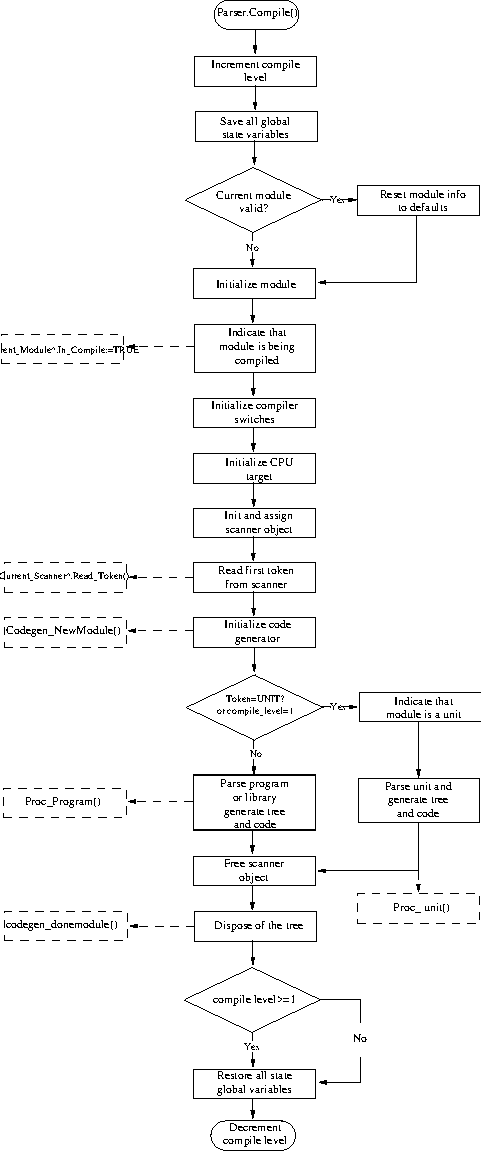
\includegraphics{arch8.pdf}
%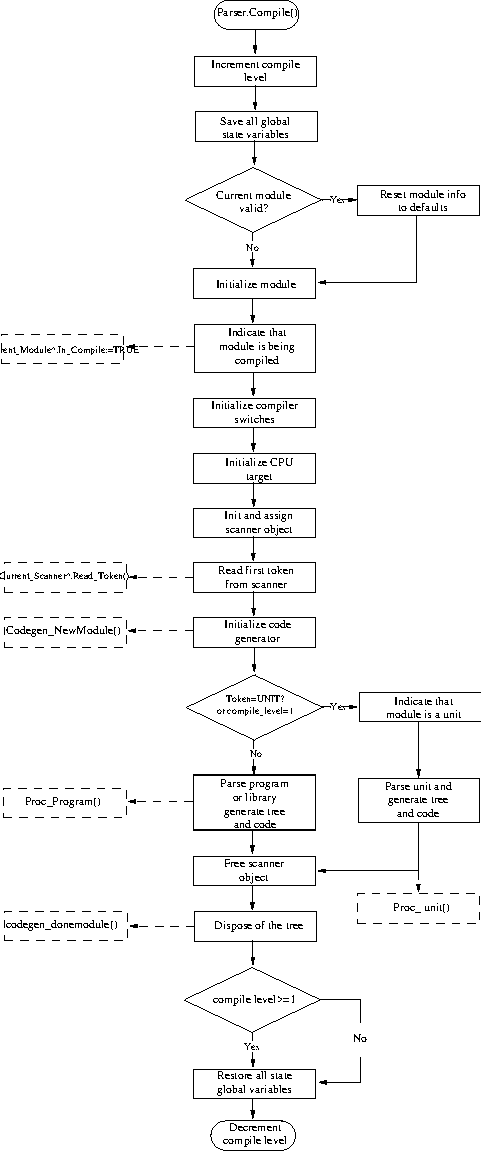
\epsfig{file=arch8.png,width=\textwidth}
\else
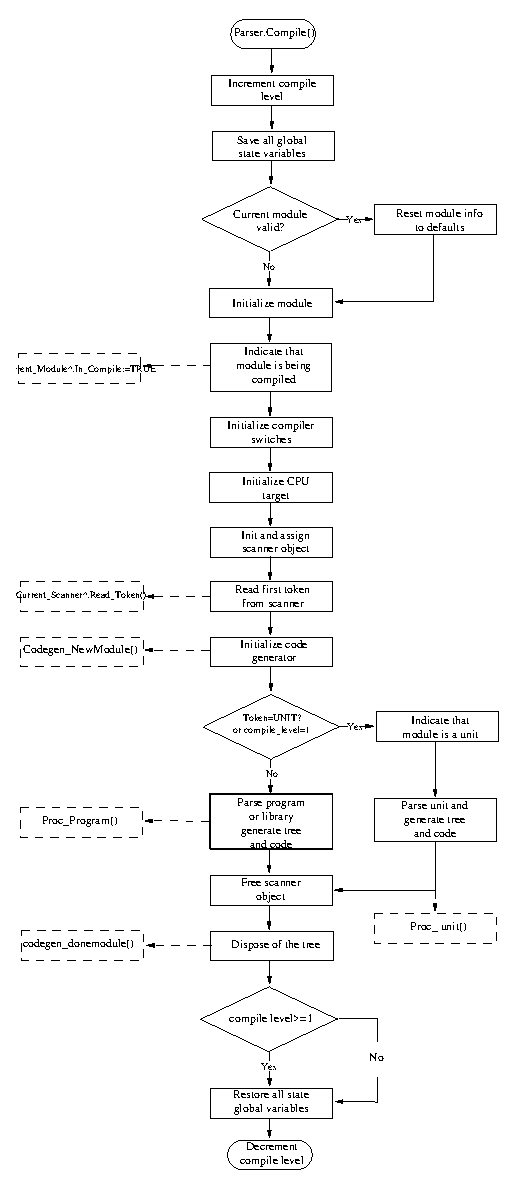
\includegraphics[width=4.99in,height=8.36in]{arch8.eps}
\fi
\label{fig8}
\caption{Parser - Scanner flow}
\end{figure}

\subsubsection{program or library parsing }

\subsubsection{unit parsing }
\label{subsubsec:mylabel12}

\subsubsection{routine parsing }
\label{subsubsec:routine}

\subsubsection{label declarations }
\label{subsubsec:mylabel13}

\subsubsection{constant declarations}
\label{subsubsec:mylabel14}

\subsubsection{type declarations}
\label{subsubsec:mylabel15}

\subsubsection{variable declarations}
\label{subsubsec:mylabel16}

\subsubsection{thread variable declarations}
\label{subsubsec:thread}

\subsubsection{resource string declarations}
\label{subsubsec:resource}

\subsubsection{exports declaration}
\label{subsubsec:exports}

\subsubsection{expression parsing }
\label{subsubsec:expression}

\subsubsection{typed constant declarations}
\label{subsubsec:mylabel17}

\subsection{Parser interface}
\label{subsec:parser}

\subsubsection{Routines}
\label{subsubsec:routinesnterfaceecla}

\subsubsection{Variables}
\label{subsubsec:variablesterfaceecla}

\paragraph{General}

\begin{variable}{AktProcSym}
\Declaration
Var aktprocsym : pProcSym;
\Description
Pointer to the symbol information for the routine currently being parsed.
\end{variable}

\begin{variable}{LexLevel}
\Declaration
var lexlevel : longint;
\Description
Level of code currently being parsed and compiled  \par 0 = for main program
\par 1 = for subroutine \par 2 = for local / nested subroutines.
\end{variable}

\begin{variablel}{Current{\_}Module}{currentmodule}
\Declaration
var Current{\_}Module : pModule;
\Description
Information on the current module (program, library or unit) being compiled.
\end{variablel}

\paragraph{Ordinal definitions}

The following variables are default type definitions which are created each
time compilation begins (default system-unit definitions), these definitions
should always be valid:

\begin{variable}{VoidDef}
\Declaration
var VoidDef : pOrdDef;
\Description
Pointer to procedure???
\Notes
This is loaded as a default supported type for the compiler
\end{variable}

\begin{variable}{cCharDef}
\Declaration
var cCharDef : pOrdDef;
\Description
Type definition for a character (\textsf{char})
\Notes
This is loaded as a default supported type for the compiler
\end{variable}

\begin{variable}{cWideCharDef}
\Declaration
var cWideCharDef : pOrdDef;
\Description
Type definition for a unicode character (\textsf{widechar})
\Notes
This is loaded as a default supported type for the compiler
\end{variable}

\begin{variable}{BoolDef}
\Declaration
var BoolDef : pOrdDef;
\Description
Type definition for a boolean value (\textsf{boolean})
\Notes
This is loaded as a default supported type for the compiler
\end{variable}

\begin{variable}{u8BitDef}
\Declaration
var u8BitDef : pOrdDef;
\Description
Type definition for an 8-nit unsigned value (\textsf{byte})
\Notes
This is loaded as a default supported type for the compiler
\end{variable}

\begin{variable}{u16BitDef}
\Declaration
var u16BitDef : pOrdDef;
\Description
Type definition for an unsigned 16-bit value (\textsf{word})
\Notes
This is loaded as a default supported type for the compiler
\end{variable}

\begin{variable}{u32BitDef}
\Declaration
var u32BitDef : pOrdDef;
\Description
Type definition for an unsigned 32-bit value (\textsf{cardinal})
\Notes
This is loaded as a default supported type for the compiler
\end{variable}

\begin{variable}{s32BitDef}
\Declaration
var s32BitDef : pOrdDef;
\Description
Type definition for a signed 32-bit value (\textsf{longint})
\Notes
This is loaded as a default supported type for the compiler
\end{variable}

\begin{variable}{cu64BitDef}
\Declaration
var cu64BitDef : pOrdDef;
\Description
Type definition for an unsigned 64-bit value (\textsf{qword})
\Notes
This is loaded as a default supported type for the compiler
\end{variable}

\begin{variable}{cs64BitDef}
\Declaration
var cs64BitDef : pOrdDef;
\Description
Type definition for a signed 64-bit value (\textsf{int64})
\Notes
This is loaded as a default supported type for the compiler
\end{variable}

\paragraph{floating point definitions}

The following variables are default type definitions which are created each
time compilation begins (default system-unit definitions), these definitions
should always be valid:

\begin{variable}{s64FloatDef}
\Declaration
var s64FloatDef : pFloatDef;
\Description
Type definition for a 64-bit IEEE floating point type (\textsf{double})
\Notes
This is loaded as a default supported type for the compiler. This might not
actually really point to the double type if the cpu does not support it.
\end{variable}

\begin{variable}{s32FloatDef}
\Declaration
var s32FloatDef : pFloatDef;
\Description
Type definition for a 32-bit IEEE floating point type (\textsf{single})
\Notes
This is loaded as a default supported type for the compiler. This might not
actually really point to the single type if the cpu does not support it.
\end{variable}

\begin{variable}{s80FloatDef}
\Declaration
var s80FloatDef : pFloatDef;
\Description
Type definition for an extended floating point type (\textsf{extended})
\Notes
This is loaded as a default supported type for the compiler. This
might not actually really point to the extended type if the cpu does not
support it.
\end{variable}

\begin{variable}{s32FixedDef}
\Declaration
var s32FixedDef : pFloatDef;
\Description
Type definition for a fixed point 32-bit value (\textsf{fixed})
\Notes
This is loaded as a default supported type for the compiler. This is
not supported officially in FPC 1.0
\end{variable}

\clearpage

\paragraph{String definitions}
The following variables are default type definitions which are created each
time compilation begins (default system-unit definitions), these definitions
should always be valid:

\begin{variable}{cShortStringDef}
\Declaration
var cShortStringDef : pStringDef;
\Description
Type definition for a short string type (\textsf{shortstring})
\Notes
This is loaded as a default supported type for the compiler.
\end{variable}

\begin{variable}{cLongStringDef}
\Declaration
var cLongStringDef : pStringDef;
\Description
Type definition for a long string type (\textsf{\textit{longstring}})
\Notes
This is loaded as a default supported type for the compiler.
\end{variable}

\begin{variable}{cAnsiStringDef}
\Declaration
var cAnsiStringDef : pStringDef;
\Description
Type definition for an ansistring type (\textsf{ansistring})
\Notes
This is loaded as a default supported type for the compiler.
\end{variable}

\begin{variable}{cWideStringDef}
\Declaration
var cWideStringDef : pStringDef;
\Description
Type definition for an wide string type (\textsf{\textit{widestring}})
\Notes
This is loaded as a default supported type for the compiler.
\end{variable}

\begin{variable}{OpenShortStringDef}
\Declaration
var OpenShortStringDef : pStringDef;
\Description
Type definition for an open string type (\textsf{openstring})
\Notes
This is loaded as a default supported type for the compiler.
\end{variable}

\begin{variable}{OpenCharArrayDef}
\Declaration
var OpenCharArrayDef : pArrayDef;
\Description
Type definition for an open char array type(\textsf{openchararray})
\Notes
This is loaded as a default supported type for the compiler.
\end{variable}

\clearpage

\paragraph{Pointer definitions}

The following variables are default type definitions which are created each
time compilation begins (default system-unit definitions), these definitions
should always be valid:

\begin{variable}{VoidPointerDef}
\Declaration
var VoidPointerDef : pPointerDef;
\Description
Type definition for a pointer which can point to anything (\textsf{pointer})
\Notes
This is loaded as a default supported type for the compiler
\end{variable}

\begin{variable}{CharPointerDef}
\Declaration
var CharPointerDef : pPointerDef;
\Description
Type definition for a pointer which can point to characters (\textsf{pchar})
\Notes
This is loaded as a default supported type for the compiler
\end{variable}

\begin{variable}{VoidFarPointerDef}
\Declaration
var VoidFarPointerDef : pPointerDef;
\Description
Type definition for a pointer which can point to anything
(intra-segment) (\textsf{far pointer})
\Notes
This is loaded as a default supported type for the compiler
\end{variable}

\begin{variable}{cFormalDef}
\Declaration
var cFormalDef : pFormalDef;
\Notes
This is loaded as a default supported type for the compiler
\end{variable}

\paragraph{Other definitions}

\begin{variable}{cfFileDef}
\Declaration
var cfFileDef : pFileDef;
\Description This is the default file type (\textsf{file})
\Notes This is loaded as a default supported type for the compiler
\end{variable}

\section{The inline assembler parser}
\label{sec:mylabel6}

\section{The code generator}
\label{sec:mylabel7}

\subsection{Introduction}
\label{subsec:introductioneratorer}

The code generator is responsible for creating the assembler output in form
of a linked list, taking as input the node created in the parser and the
1$^{st}$ pass. The following diagram shows an overview of the code generator
architecture:

\begin{figure}
\ifpdf
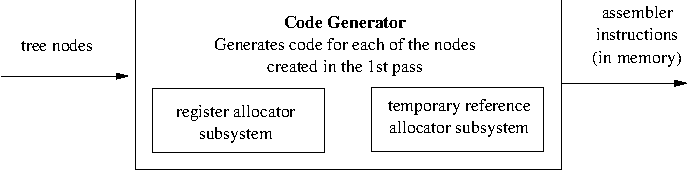
\includegraphics{arch9.pdf}
%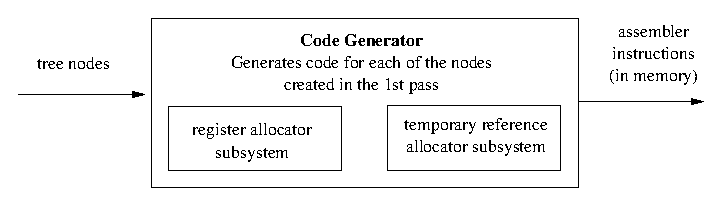
\epsfig{file=arch9.png,width=\textwidth}
\else
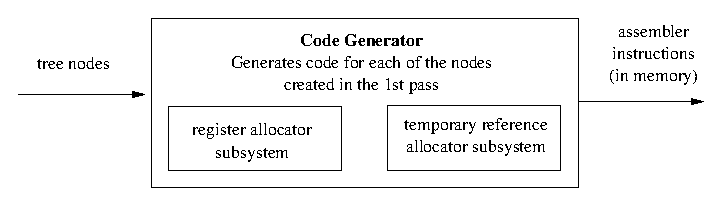
\includegraphics[width=5.68in,height=1.76in]{arch9.eps}
\fi
\label{fig9}
\caption{Codegenerator architecture}
\end{figure}

The code generation is only done when a procedure body is parsed; the
interaction, between the 1$^{st}$ pass (type checking phase), the code
generation and the parsing process is show in the following diagram:

\begin{figure}
\ifpdf
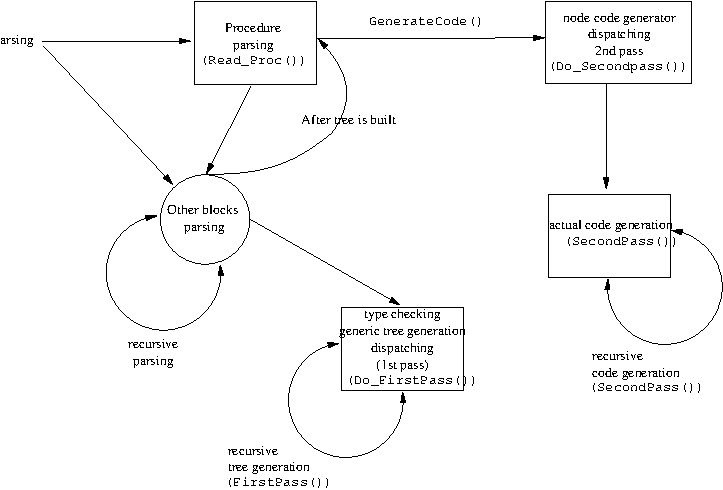
\includegraphics{arch10.pdf}
%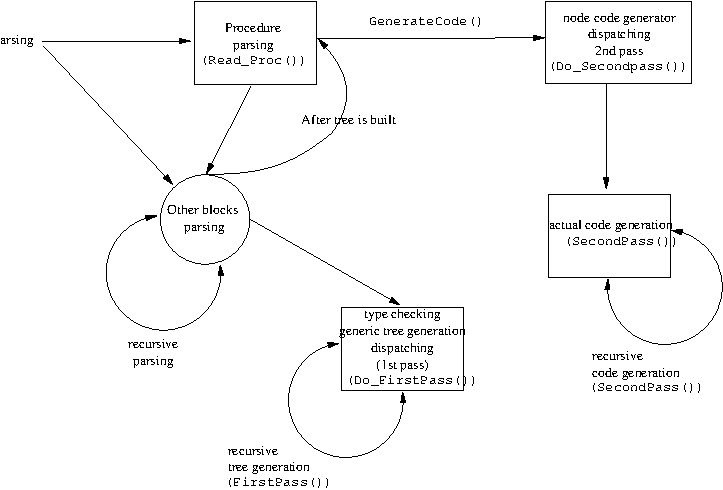
\epsfig{file=arch10.png,width=\textwidth}
\else
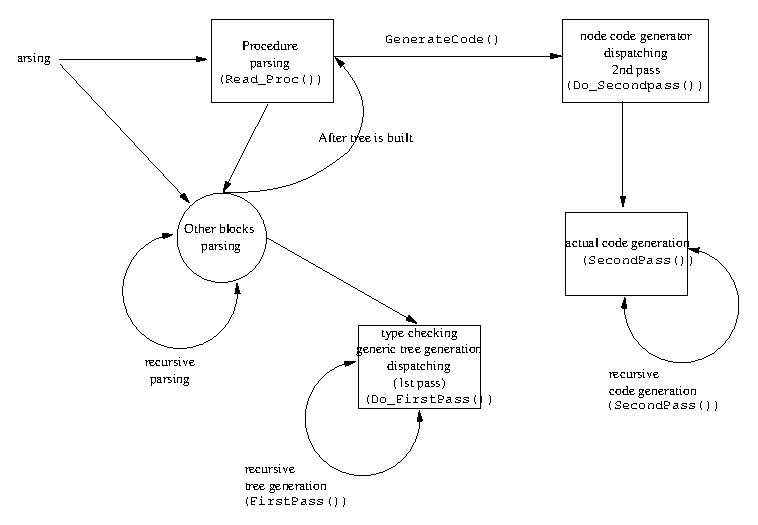
\includegraphics[width=6.95in,height=4.90in]{arch10.eps}
\fi
\label{fig10}
\caption{Interaction between codegeneration and the parsing process}
\end{figure}

The \textsf{secondpass()} is actually a simple dispatcher. Each possible
tree type node (Cf. Tree types) is associated with
a second pass routine which is called using a dispatch table.

\subsection{Locations (cpubase.pas)}
\label{subsec:locations}

The code generator uses the tree location component to indicate the location
where the current node operands are located. This is then used by the code
generator to generate the appropriate instruction, all depending on the
location of the operand. The possible operand locations:

\begin{longtable}{|l|p{10cm}|}
\hline
Location define & Description \\
\hline
\endhead
\hline
\endfoot
\textsf{LOC{\_}INVALID}&
    Invalid location (should never occur) \\
\textsf{LOC{\_}FPU}&
    Floating point registers \\
\textsf{LOC{\_}REGISTER}&
    Integer registers \\
\textsf{LOC{\_}MEM}&
    Memory Location \\
\textsf{LOC{\_}REFERENCE}&
    Constant node with constant value \\
\textsf{LOC{\_}JUMP}&
    Label operand \\
\textsf{LOC{\_}FLAGS}&
    Flags operand \\
\textsf{LOC{\_}CREGISTER}&
    Constant integer register (when operand is in this
    location, it should be considered as read-only) \\
\end{longtable}

Depending on the location type, a variable structure is defined indicating
more information on the operand. This is used by the code generator to
generate the exact instructions.

\subsubsection{LOC{\_}INVALID}
\label{subsubsec:mylabel18}

This location does not contain any related information, when this location
occurs, it indicates that the operand location was not initially allocated
correctly. This indicates a problem in the compiler.

\subsubsection{LOC{\_}FPU}
\label{subsubsec:mylabel19}

This indicates a location in the coprocessor; this is platform dependant.

\paragraph{Stack based FPU}

Only one CPU uses a stack based FPU architecture, this is the intel 80x86
family of processors. When the operand is on the top of the stack, the
operand is of type LOC{\_}FPU.

\paragraph{Register based FPU}

When the floating point co-processor is register based, the following
field(s) are defined in the structure to indicate the current location of
the operand:

\begin{longtable}{|l|p{7cm}|}
\hline
Field   & Description \\
\hline
\endhead
\hline
\endfoot
\textsf{fpuregister : tregister;}&
    Indicates in what register the operand is located (a general purpose
    register in emulation mode, and a floating point register when floating
    point hardware is present) \\
\textsf{fpuregisterhigh, } \par \textsf{fpuregisterlow : tregister;}&
    Indicates in what registers the operand are located (for emulation
    support - these are general purpose registers)
\end{longtable}

\subsubsection{LOC{\_}REGISTER}
\label{subsubsec:mylabel20}

This fields indicates that the operand is located in a CPU register. It is
possible to allocate more then one register, if trying to access 64-bit
values on 32-bit wide register machines.

\begin{longtable}{|l|p{10cm}|}
\hline
Field   & Description \\
\hline
\endhead
\hline
\endfoot
\textsf{register : tregister}&
    Indicates in what register the operand is located. \\
\textsf{registerhigh : tregister;}&
    High 32-bit of 64-bit virtual register (on 32-bit machines) \\
\textsf{registerlow : tregister;}&
    Low 32-bit of 64-bit virtual register (on 32-bit machines)
\end{longtable}

\subsubsection{LOC{\_}MEM, LOC{\_}REFERENCE}
\label{subsubsec:mylabel21}

This either indicates an operand in memory, or a constant integer numeric
value. The fields for this type of operand is as follows:

\begin{longtable}{|l|p{10cm}|}
\hline
Field   & Description \\
\hline
\endhead
\hline
\endfoot
\textsf{reference : treference;}&
    Information on the location in memory
\end{longtable}

References are the basic building blocks of the code generator, every load
and store in memory is done via a reference. A reference type can either
point to a symbolic name, an assembler expression (base register + index
register + offset)*scale factor, as well as simply giving information on a
numeric value.

The treference consists of the following:

\begin{tabular*}{6.5in}{|l@{\extracolsep{\fill}}lp{6,5cm}|}
\hline
\textsf{TYPE} & & \\
\xspace \textsf{pReference} &= \^{} \textbf{TReference};&  \\
\xspace \textsf{TReference} &= \textbf{packed Record} & \\
&\textsf{is{\_}immediate : boolean;}&
    Indicates that this location points to a memory location, but to a
    constant value (TRUE), which is located in the offset field. \\
&\textsf{segment : tregister;}& (cpu-specific) \\
&\textsf{base : tregister;}&
    Base address register for assembler expression \\
&\textsf{index : tregister;}&
    Index register for assembler expression \\
&\textsf{scalefactor : byte;}&
    Multiplication factor for assembler expression (this field is
    cpu-specific) \\
&\textsf{offset : longint;}&
    Either an offset from base assembler address expression to add (if
    is{\_}constant = FALSE) otherwise the numeric value of the operand \\
&\textsf{symbol : pasmsymbol;}&
    Pointer to the symbol name string of the reference in case where it is
    a symbolic reference \\
&\textsf{offsetfixup : longint;}&  \\
&\textsf{options : trefoptions;}&  \\
&\textsf{END;}&  \\
\hline
\end{tabular*}

\subsubsection{LOC{\_}JUMP}
\label{subsubsec:mylabel22}

There are no fields associated with this location, it simply indicates that
it is a boolean comparison which must be done to verify the succeeding
operations. (i.e the processor zero flag is valid and gives information on
the result of the last operation).

\subsubsection{LOC{\_}FLAGS}
\label{subsubsec:mylabel23}

The operand is in the flags register. From this operand, the conditional
jumps can be done. This is processor dependant, but normally the flags for
all different comparisons should be present.

\begin{longtable}{|l|p{10cm}|}
\hline
Field   & Description \\
\hline
\endhead
\hline
\endfoot
\textsf{resflags : tresflags;}&
    This indicates the flag which must be verified for the actual jump
    operation. \textsf{tresflags }is an enumeration of all possible
    conditional flags which can be set by the processor. \\
\end{longtable}

\subsubsection{LOC{\_}CREGISTER}
\label{subsubsec:mylabel24}

This is a read-only register allocated somewhere else in the code generator.
It is used mainly for optimization purposes. It has the same fields as
LOC{\_}REGISTER, except that the registers associated with this location can
only be read from, and should never be modified directly.

\begin{longtable}{|l|p{10cm}|}
\hline
Field   & Description \\
\hline
\endhead
\hline
\endfoot
\textsf{register : tregister}&
    Indicates in what register the operand is located. \\
\textsf{registerhigh : tregister;}&
    High 32-bit of 64-bit virtual register (on 32-bit machines) \\
\textsf{registerlow : tregister;}&
    Low 32-bit of 64-bit virtual register (on 32-bit machines) \\
\end{longtable}

\subsubsection{LOCATION PUBLIC INTERFACE}
\label{subsubsec:location}

\begin{procedurel}{Del{\_}Location}{dellocation}
\Declaration
procedur Del{\_}Location(const L : TLocation);
\Description
If the location points to a LOC{\_}REGISTER or LOC{\_}CREGISTER, it frees up
the allocated register(s) associated with this location. If the location
points to LOC{\_}REFERENCE or LOC{\_}MEM, it frees up the the allocated base
and index registers associated with this node.
\end{procedurel}

\begin{procedurel}{Clear{\_}Location}{clearlocation}
\Declaration
procedure Clear{\_}location(var Loc : TLocation);
\Description
Sets the location to point to a LOC{\_}INVALID type.
\end{procedurel}

\begin{procedurel}{Set{\_}Location}{setlocation}
\Declaration
procedure Set{\_}Location(var Destloc,Sourceloc : TLocation);
\Description
The destination location now points to the destination location (now copy is
made, a simple pointer assignment)
\end{procedurel}

\begin{procedurel}{Swap{\_}Location}{swaplocation}
\Declaration
Procedure Swap{\_}Location(var Destloc,Sourceloc : TLocation);
\Description
Swap both location pointers.
\end{procedurel}

\subsection{Registers (cpubase.pas)}
\label{subsec:registers}

The code generator defines several types of registers which are categorized
by classes. All (except for the scratch register class) of these register
classes are allocated / freed on the fly, when the code is generated in the
code generator: The registers are defined in a special enumeration called
tregister. This enumeration contains all possible register defines for the
target architecture, and a possible definition could be as follows :

% FIXME this should be changed to something more TeXish

\textsf{tregister = (}

\textsf{{\{} general purpose registers {\}} }

\textsf{R{\_}NO,R{\_}D0,R{\_}D1,R{\_}D2,R{\_}D3,R{\_}D4,R{\_}D5,R{\_}D6,R{\_}D7,}

\textsf{{\{} address registers {\}}}

\textsf{R{\_}A0,R{\_}A1,R{\_}A2,R{\_}A3,R{\_}A4,R{\_}A5,R{\_}A6,R{\_}SP,}

\textsf{{\{} PUSH/PULL- quick and dirty hack {\}}}

\textsf{R{\_}SPPUSH,R{\_}SPPULL,}

\textsf{{\{} misc. and floating point registers {\}}}

\textsf{R{\_}CCR,R{\_}FP0,R{\_}FP1,R{\_}FP2,R{\_}FP3,R{\_}FP4,R{\_}FP5,R{\_}FP6,}

\textsf{R{\_}FP7,R{\_}FPCR,R{\_}SR,R{\_}SSP,R{\_}DFC,R{\_}SFC,R{\_}VBR,R{\_}FPSR,}

\textsf{{\{} other - not used {\}}}

\textsf{R{\_}DEFAULT{\_}SEG}

\textsf{);}

\subsubsection{integer registers}
\label{subsubsec:integer}

\textsf{intregs: array[1..maxintregs] of tregister;}

General purpose registers which can contain any data, usually integer
values. These can also be used, when no floating point coprocessor is
present, to hold values for floating point operations.

\subsubsection{address registers}
\label{subsubsec:address}

\textsf{addrregs: array[1..maxaddrregs] of tregister;}

Registers which are used to construct assembler address expressions, usually
the address registers are used as the base registers in these assembler
expressions.

\subsubsection{fpu registers}
\label{subsubsec:mylabel25}

\textsf{fpuregs: array[1..maxfpuregs] of tregister;}

Hardware floating point registers. These registers must at least be able to
load and store IEEE DOUBLE floating point values, otherwise they cannot be
considered as FPU registers. Not available on systems with no floating point
coprocessor.

\subsubsection{scratch registers}
\label{subsubsec:scratch}

\textsf{scratch{\_}regs: array[1..maxscratchregs] of tregister;}

These registers are used as scratch, and can be used in assembler statement
in the pascal code, without being saved. They will always be valid across
routine calls. These registers are sometimes temporarily allocated inside
code generator nodes, and then immediately freed (always inside the same
routine).

\subsection{Special registers (cpubase.pas)}
\label{subsec:special}

The code generator has special uses for certain types of registers. These
special registers are of course CPU dependant, but as an indication, the
following sections explains the uses of these special registers and their
defines.

\subsubsection{stack{\_}pointer}
\label{subsubsec:stack}

\textsf{const stack{\_}pointer = R{\_}A7}

This represents the stack pointer, an address register pointing to the
allocated stack area.

\subsubsection{frame{\_}pointer}
\label{subsubsec:frame}

\textsf{const frame{\_}pointer = R{\_}A6}

This represents the frame register which is used to access values in the
stack. This is usually also an address register.

\subsubsection{self{\_}pointer}
\label{subsubsec:mylabel26}

\textsf{const self{\_}pointer = R{\_}A5}

This represents the self register, which represents a pointer to the current
instance of a class or object.

\subsubsection{accumulator}
\label{subsubsec:accumulatorents}

\textsf{const accumulator = R{\_}D0}

The accumulator is used (except in the i386) as a scratch register, and also
for return value in functions (in the case where they are 32-bit or less).
In the case it is a 64-bit value (and the target processor only supports
32-bit registers) , the result of the routine is stored in the accumulator
for the low 32-bit value, and in the scratch register
(\textsf{scratch{\_}register}) for the high 32-bit value.

\subsubsection{scratch register}
\label{subsubsec:mylabel27}

\textsf{const scratch{\_}reg = R{\_}D1}

This register is used in special circumstances by the code generator. It is
simply a define to one of the registers in the \textsf{scratch{\_}regs
}array.

\subsection{Instructions}
\label{subsec:instructionsr}

\subsection{Reference subsystem}
\label{subsec:reference}

\subsubsection{Architecture}
\label{subsubsec:architecturebsysteme}

As described before in the locations section, one of the possible locations
for an operand is a memory location, which is described in a special
structure \textsf{treference} (described earlier). This subsection describes
the interface available by the code generator for allocation and freeing
reference locations.

\subsubsection{Code generator interface}
\label{subsubsec:mylabel28}

\lstinline!Function NewReference(Const R : TReference) : pReference;!

\begin{procedure}{DisposeReference}
\Declaration
Procedure DisposeReference(Var R : pReference);
\Description
Disposes of the reference \textsf{R} and sets r to \textsf{NIL}
\Notes
Does not verify if \textsf{R} is assigned first.
\end{procedure}

\begin{function}{NewReference}
\Declaration
function NewReference(Const R : TReference) : pReference;
\Description
Allocates in the heap a copy of the reference \textsf{r} and returns that
allocated pointer.
\end{function}

\begin{functionl}{Del{\_}Reference}{delreference}
\Declaration
procedure Del{\_}Reference(Const Ref : tReference);
\Description
Free up all address registers allocated in this reference for the index and
base (if required).
\Notes
Does not free the reference symbol if it exists.
\end{functionl}

\begin{functionl}{New{\_}Reference}{resetreference}
\Declaration
Function New{\_}Reference(Base : TRegister;Offset : Longint) : PReference;
\Description
Allocates a reference pointer, clears all the fields to zero, and sets the
offset to the offset field and the base to the base fields of the newly
allocated reference. Returns this newly allocated reference.
\end{functionl}

\begin{procedurel}{Reset{\_}Reference}{resetreference}
\Declaration
procedure Reset{\_}Reference(var ref : treference);
\Description
Clears all fields of the reference.
\end{procedurel}

\subsection{The register allocator subsystem}
\label{subsec:mylabel7}

\subsubsection{Architecture}
\label{subsubsec:architecture}

This system allocates and deallocates registers, from a pool of free
registers. Each time the code generator requires a register for generating
assembler instructions, it either calls the register allocator subsystem to
get a free register or directly uses the scratch registers (which are never
allocated in a pool except in the optimization phases of the compiler).

The code generator when no longer referencing the register should deallocate
it so it can be used once again.

\subsubsection{Code generator interface (tgen.pas)}
\label{subsubsec:mylabel29}

The following interface routines are used by the code generator to allocate
and deallocate registers from the different register pools available to code
generator.

\paragraph{General purpose registers}

\begin{function}{GetRegister32}
\Declaration
function GetRegister32 : tregister;
\Description
Allocates and returns a general purpose (integer) register which can be used
in the code generator. The register, when no longer used should be
deallocated with ungetregister32() or ungetregister()
\Notes
On non 32-bit machines, this routine should return the normal register for
this machine (eg : 64-bit machines will alloate and return a 64-bit
register).
\end{function}

\begin{procedure}{GetRegisterPair}
\Declaration
procedure GetRegisterPair(var low, high : TRegister);
\Description
Returns a register pair to be used by the code generator when accessing
64-bit values on 32-bit wide register machines.
\Notes
On machines which support 64-bit registers naturally, this routine should
never be used, it is intended for 32-bit machines only.par Some machines
support 64-bit integer operations using register 32-bit pairs in hardware,
but the allocated registers must be specific, this routine is here to
support these architectures.
\end{procedure}

\begin{procedure}{UngetRegister32}
\Declaration
Procedure UnGetRegister32(R : TRegister);
\Description
Deallocates a general purpose register which was previously allocated with
\seef{GetRegister32}().
\end{procedure}

\paragraph{Floating point registers}

\begin{function}{GetFloatRegister}
\Declaration
Function GetFloatRegister : tregister;
\Description
Allocates and returns a floating point register which can be used in the
code generator. The register, when no longer used should be deallocated with
ungetregister(). The register returned is a true floating point register (if
supported).
\Notes
This routine should only be used when floating point hardware is present in
the system. For emulation of floating point, the general purpose register
allocator / deallocator routines should be used instead.
\end{function}

\begin{function}{IsFloatsRegister}
\Declaration
Function IsFloatsRegister(R : TRegister): Boolean;
\Description
Returns TRUE if the register r is actually a floating point register,
otherwise returns FALSE. This is used when the location is LOC{\_}FPU on
machines which do not support true floating point registers.
\end{function}

\paragraph{Address registers}

\begin{function}{GetAdressReg}
\Declaration
Function GetAddressReg : tregister;
\Description
Allocates and returns an address register which can be used for address
related opcodes in the code generator. The register, when no longer used
should be deallocated with ungetregister()
\Notes
If there is no distinction between address registers, and general purpose
register in the architecture, this routine may simply call and return the
getregister32() result.
\end{function}

\begin{function}{IsAddressRegister}
\Declaration
Function IsAddressRegister(r : TRegister): Boolean;
\Description
Returns TRUE if the register r is actually an address register, otherwise
returns FALSE.
\Notes
If there is no distinction between address registers, and general purpose
register in the architecture, this routine may simply verify if this is a
general purpose register and return TRUE in that case.
\end{function}

\paragraph{Generic}

\begin{procedure}{UngetRegister}
\Declaration
procedure UngetRegister(r : TRegister);
\Description
Deallocates any register which was previously allocated with any of the
allocation register routines.
\end{procedure}

\begin{function}{SaveUsedRegisters}
\Declaration
procedure SaveUsedRegisters(var Saved : TSaved; ToSave: TRegisterset);
\Description
Saves in a temporary location all specified registers. On stack based
machines the registers are saved on the stack, otherwise they are saved in a
temporary memory location. The registers which were saved are stored in the
\textsf{saved} variable. The constant \textsf{ALL{\_}REGISTERS} passed to
the \textsf{tosave} parameter indicates to save all used registers.
\end{function}

\begin{function}{RestoreUsedRegisters}
\Declaration
procedure restoreusedregisters(Saved : TSaved);
\Description
Restores all saved registers from the stack (or a temporary memory
location). Free any temporary memory space allocated, if necessary.
\end{function}

\paragraph{Debugging}

\begin{function}{GetExplicitRegister32}
\Declaration
Function GetExplicitRegister32(r : tregister): tregister;
\Description
This routine allocates specifically the specified register \textsf{r }and
returns that register. The register to allocate can only be one of the
scratch registers.
\Notes
This routine is used for debugging purposes only. It should be used in
conjunctions with ungetregister32() to explicitly allocate and deallocate a
scratch register.
\end{function}

\subsection{Temporary memory allocator subsystem}
\label{subsec:temporary}

\subsubsection{Architecture}
\label{subsubsec:architecturemory}

Sometimes it is necessary to reserve temporary memory locations on the stack
to store intermediate results of statements. This is done by the temporary
management module.

Since entry and exit code for routines are added after the code for the
statements in the routine have been generated, temporary memory allocation
can be used `on the fly' in the case where temporary memory values are
required in the code generation phase of the routines being compiled. After
usage, the temporary memory space should be freed, so it can be reused if
necessary.

The temporary memory allocation is a linked list of entries containing
information where to access the data via a negative offset from the
frame{\_}pointer register. The linked list is only valid when compiling and
generating the code for the procedure bodies; it is reset and cleared each
time a new routine is compiled. There are currently three different types of
memory spaces in use : volatile (\textsf{tt{\_}normal}) which can be
allocated and freed any time in the procedure body, ansistring, which is
currently the same as volatile, except it only stored references to
ansistring's, and persistent (\textsf{tt{\_}persistent}) which are memory
blocks which are reserved throughout the routine duration; persistent
allocated space can never be reused in a procedure body, unless explicitly
released.

The temporary memory allocator guarantees to allocate memory space on the
stack at least on a 16-bit alignment boundary. The exact alignment depends
on the operating system required alignment.

\subsubsection{Temporary memory allocator interface (temp{\_}gen.pas)}
\label{subsubsec:temporary}

\paragraph{volatile / ansistring memory}

\begin{function}{GetTempOfSize}
\Declaration
function GetTempOfSize(Size : Longint) : Longint;
\Description
Allocates at least \textsf{size} bytes of temporary volatile memory on the
stack. The return value is the negative offset from the frame pointer where
this memory was allocated.
\Notes
The return offset always has the required alignment for the target system,
and can be used as an offset from the frame{\_}pointer to access the
temporary space.
\end{function}

\begin{procedure}{GetTempOfSizeReference}
\Declaration
procedure GetTempOfSizeReference(l : Longint;Var Ref : TReference);
\Description
This routine is used to assign and allocate extra temporary volatile memory
space on the stack from a reference. \textsf{l} is the size of the
persistent memory space to allocate, while \textsf{ref} is a reference entry
which will be set to the correct offset from the frame{\_}pointer register
base. The \textsf{offset} and \textsf{base} fields of \textsf{ref} will be
set appropriately in this routine, and can be considered valid on exit of
this routine.
\Notes
The return offset always has the required alignment for the target system.
\end{procedure}

\begin{procedure}{UnGetIfTemp}
\Declaration
procedure UnGetIfTemp(const ref : treference);
\Description
Frees a reference \textsf{ref} which was allocated in the volatile temporary
memory space. 
\Notes
The freed space can later be reallocated and reused.
\end{procedure}

\begin{procedure}{GetTempAnsiStringReference}
\Declaration
procedure GetTempAnsiStringReference(Var Ref : TReference);
\Description
Allocates \textsf{ref }on the volatile memory space and sets the
\textsf{base} to the frame{\_}pointer register and \textsf{offset} to the
correct offset to access this allocated memory space.
\Notes
The return offset always has the required alignment for the target system.
\end{procedure}

\paragraph{persistent memory}

\begin{function}{GetTempOfSizePersistant}
\Declaration
function GetTempOfSizePersistant(Size : Longint) :Longint;
\Description
Allocates persistent storage space on the stack. return value is the
negative offset from the frame pointer where this memory was allocated.
\Notes
The return offset always has the required alignment for the target system.
\end{function}

\begin{function}{UngetPersistantTemp}
\Declaration
procedure UngetPersistantTemp(Pos : Longint);
\Description
Frees space allocated as being persistent. This persistent space can then
later be used and reallocated. \textsf{pos} is the offset relative to the
frame{\_}pointer of the persistent memory block to free.
\end{function}

\paragraph{utility routines}

\begin{procedure}{ResetTempGen}
\Declaration
procedure ResetTempGen;
\Description
Clear and free the complete linked list of temporary memory locations. The
list is set to nil.
\Notes
This routine is called each time a routine has been fully compiled.
\end{procedure}

\begin{procedure}{SetFirstTemp}
\Declaration
procedure SetFirstTemp(l : Longint);
\Description
This routine sets the start of the temporary local area (this value is a
negative offset from the frame{\_}pointer, which is located after the local
variables). Usually the start offset is the size of the local variables,
modified by any alignment requirements.
\Notes
This routine is called once before compiling a routine, it indicates the
start address where to allocate temporary memory space.
\end{procedure}

\begin{function}{GetFirstTempSize}
\Declaration
function GetFirstTempSize : longint;
\Description
Returns the total number of bytes allocated for local and temporary
allocated stack space. This value is aligned according to the target system
alignment requirements, even if the actual size is not aligned.
\Notes
This routine is used by the code generator to get the total number of bytes
to allocate locally (i.e the stackframe size) in the entry and exit code of
the routine being compiled.
\end{function}

\begin{function}{NormalTempToPersistant}
\Declaration
Procedure NormalTempToPersistant(Pos : Longint);
\Description
Searches the list of currently temporary memory allocated for the one with
the offset \textsf{pos, }and if found converts this temporary memory space
as persistent (can never be freed and reallocated).
\end{function}

\begin{function}{PersistantTempToNormal}
\Declaration
Procedure PersistantTempToNormal(Pos : Longint);
\Description
Searches the list of currently allocated persistent memory space as the
specified address \textsf{pos }, and if found converts this memory space to
normal volatile memory space which can be freed and reused.
\end{function}

\begin{function}{IsTemp}
\Declaration
function IsTemp(const Ref : TReference): boolean;
\Description
Returns TRUE if the reference \textsf{ref }is allocated in temporary
volatile memory space, otherwise returns FALSE.
\end{function}

\subsection{Assembler generation}
\label{subsec:mylabel8}

\subsubsection{Architecture}
\label{subsubsec:architectureneration}

The different architectures on the market today only support certain types
of operands as assembler instructions. The typical format of an assembler
instruction has the following format:

\begin{center}
\textsf{OPCODE [opr1,opr2[,opr3][\ldots ]]}
\end{center}

The opcode field is a mnemonic for a specific assembler instruction, such as
\textsf{MOV} on the 80x86, or \textsf{ADDX} on the 680x0. Furthermore, in
most cases, this mnemonic is followed by zero to three operands which can be
of the following types:

Possible Operand Types
\begin{itemize}
\item a LABEL or SYMBOL (to code or data)
\item a REGISTER (one of the predefined hardware registers) 
\item a CONSTANT (an immediate value)
\item a MEMORY EXPRESSION (indirect addressing through offsets, symbols, and
     address registers)
\end{itemize}

In the compiler, this concept of different operand types has been directly
defined for easier generation of assembler output. All opcodes generated by
the code generator are stored in a linked list of opcodes which contain
information on the operand types, The opcode and the size (which is
important to determine on what size the operand must be operated on) are
stored in that linked list.

The possible operand sizes for the code generator are as follows (a
enumeration of type \textsf{topsize}):

\begin{longtable}{|l|p{10cm}|}
\hline
Operand size enum (\textsf{topsize}) & Description \\
\hline
\endhead
\hline
\endfoot
\textsf{S{\_}B}& 			8-bit integer operand \\
\textsf{S{\_}W}& 			16-bit integer operand \\
\textsf{S{\_}L}& 			32-bit integer operand \\
\textsf{S{\_}Q}& 			64-bit integer operand \\
\textsf{S{\_}FS}& 			32-bit IEEE 754 Single floating point operand \\
\textsf{S{\_}FL}& 			64-bit IEEE 754 Double floating point operand \\
\textsf{S{\_}FX}& 			Extended point floating point operand (cpu-specific) \\
\textsf{S{\_}CPU}&			A constant equal to one of the previous sizes (natural size of operands) \\
\end{longtable}

The possible operand types for the code generator are as follows (other
might be added as required by the target architecture):

\begin{longtable}{|l|p{10cm}|}
\hline
Operand type (\textsf{toptype}) & Description \\
\hline
\endhead
\hline
\endfoot
\textsf{top{\_}none}& 			No operand \\
\textsf{top{\_}reg}& 			Operand is a register \\
\textsf{top{\_}ref}& 			Operand is a reference (\textsf{treference} type) \\
\textsf{top{\_}symbol}& 		Operand is a symbol (reference or label) \\
\end{longtable}

The architecture specific opcodes are done in an enumeration of type
\textsf{tasmop}. An example of an enumeration for some of the opcodes of the
PowerPC 32-bit architecture is as follows:

\begin{lstlisting}{}
type tasmop = (a_add, a_add_, a_addo, a_addo_, a_addc, a_addc_, a_addco,
	       a_addco_,a_adde, a_adde_, a_addeo, a_addeo_, a_addi,
	       a_addic, a_addic_, a_addis \ldots
\end{lstlisting}

\subsubsection{Generic instruction generation interface}
\label{subsubsec:generic}

To independently generate code for different architectures, wrappers for the
most used instructions in the code generator have been created which are
totally independent of the target system.

\paragraph{Load / store instructions}

\begin{procedurel}{Emit\_Load\_Loc\_Reg}{EmitLoadLocReg}
\Declaration
Procedure Emit{\_}Load{\_}Loc{\_}Reg(src:tlocation;srcdef:pdef; dstdef : pdef; dst : tregister);
\Description
Loads an operand from the source location in \textsf{src }into the
destination register \textsf{dst }taking into account the source definition
and destination definition (sign-extension, zero extension depending on the
sign and size of the operands).
\Notes
The source location can only be in LOC{\_}REGISTER, LOC{\_}CREGISTER,
LOC{\_}MEM or LOC{\_}REFERENCE otherwise an internal error will occur. This
generic opcode does not work on floating point values, only integer values.
\end{procedurel}

\begin{procedure}{FloatLoad}
\Declaration
procedure FloatLoad(t : tFloatType;Ref : TReference; Var Location:TLocation);
\Description
This routine is to be called each time a location must be set to LOC{\_}FPU
and a value loaded into a FPU register
\Notes
The routine sets up the register field of LOC{\_}FPU correctly. The source
location can only be : LOC{\_}MEM or LOC{\_}REFERENCE. The destination
location is set to LOC{\_}FPU.
\end{procedure}

\begin{function}{FloatStore}
\Declaration
procedure FloatStore(t : TFloatType;var Location:TLocation; ref:TReference);
\Description
This routine is to be called when a value located in LOC{\_}FPU must be
stored into memory.
\Notes
The destination must be LOC{\_}REFERENCE or LOC{\_}MEM. This routine frees
the LOC{\_}FPU location \\
\end{function}

\begin{functionl}{emit{\_}mov{\_}ref{\_}reg64}{emitmovrefreg64}
\Declaration
Procedure Emit{\_}Mov{\_}Ref{\_}Reg64(r : TReference;rl,rh : TRegister);
\Description
This routine moves a 64-bit integer value stored in memory location
\textsf{r} into the low 32-bit register \textsf{rl} and the high 32-bit
register \textsf{rh}.
\end{functionl}

\paragraph{Load address}

\begin{functionl}{Emit{\_}Lea{\_}Loc{\_}Ref}{emitlealocref}
\Declaration
procedure Emit{\_}Lea{\_}Loc{\_}Ref(const t:TLocation;Const Ref:TReference; FreeTemp:Boolean);
\Description
Loads the address of the location \textsf{loc }and stores the result into
\textsf{ref}
\Notes
The store address \textsf{ref }should point to an allocated area at least
\textsf{sizeof(pointer)} bytes, otherwise unexpected code might be
generated.
\end{functionl}

\begin{functionl}{Emit{\_}Lea{\_}Loc{\_}Reg}{Emitlealocreg}
\Declaration
Procedure Emit{\_}Lea{\_}Loc{\_}Reg(const t:TLocation;Reg:TRegister;Freetemp:Boolean);
\Description
Loads the address of the location \textsf{loc }and stores the result into
ther target register \textsf{reg}
\end{functionl}

\paragraph{Label instructions}

\begin{procedure}{GetLabel}
\Declaration
procedure GetLabel(var l : pAsmLabel);
\Description
Returns a label associated with code. This label can then be used with the
instructions output by the code generator using the instruction generation
templates which require labels as parameters. The label itself can be
emitted to the assembler source by calling the \textsf{emitlab} routine.
\end{procedure}

\begin{procedure}{EmitLab}
\Declaration
procedure EmitLab(var l : pasmlabel);
\Description
Output the label \textsf{l }to the assembler instruction stream.
\Notes
The label should have been previously allocated with \textsf{getlabel.} The
output label will be of the form label: in the instruction stream. This
label is usually a jump target.
\end{procedure}

\begin{procedure}{EmitLabeled}
\Declaration
procedure EmitLabeled(op : tasmop; var l : pasmlabel);
\Description
Output the opcode \textsf{op }with the operand \textsf{l}
which is a previously allocated label.
\Notes
This routine is used to output jump instructions such as : jmp label, jne
label.  The label should have been previously allocated with a call to
\textsf{getlabel}

\end{procedure}

\paragraph{Other instructions}

\begin{function}{EmitCall}
\Declaration
procedure EmitCall(const routine:string);
\Description
Emit a call instruction to an internal routine
\Parameters
routine = The name of the routine to call.
\end{function}

\begin{procedure}{ConcatCopy}
\Declaration
procedure ConcatCopy(Source,Dest : TReference;Size : Longint;DelSource : Boolean; loadref:boolean);
\Description
This routine copies \textsf{size} data from the \textsf{source} reference to the destination \textsf{dest} reference. \\
\Parameters
source = Source reference to copy from \par
dest = Depending on the value of loadref, either indicates a location where a
pointer to the data to copy is stored, or this reference directly the address
to copy to. \par
size = Number of bytes to copy \par delsource = TRUE if the source reference
should be freed in this routine \par loadref = TRUE if the source reference
contains a pointer to the address we wish to copy to, otherwise the reference
itself is the destination location to copy to.
\end{procedure}

\begin{procedurel}{Emit{\_}Flag2Reg}{emitflag2reg}
\Declaration
procedure Emit{\_}Flag2Reg(Flag:TResflags;HRegister:TRegister);
\Description
Sets the value of the register to 1 if the condition code flag in \textsf{flag}
is TRUE, otherwise sets the register to zero.
\Notes
The operand should be zero extended to the natural register size for the
target architecture.
\end{procedurel}

\subsubsection{Instruction generation interface}
\label{subsubsec:instruction}

\section{The assembler output}
\label{sec:mylabel8}

All code is generated via special linked lists of instructions. The base of
this is a special object, an abstract assembler which implements all
directives which are usually implemented in the different assemblers
available on the market . When the code generator and parser generates the
final output, it is generated as a linked list for each of the sections
available for the output assembler. Each entry in the linked list is either
an instruction, or one of the abstract directives for the assembler.

\begin{figure}
\ifpdf
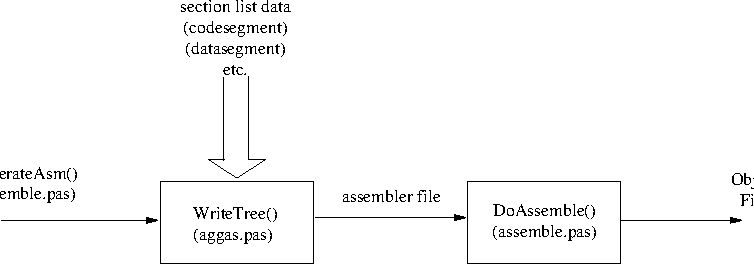
\includegraphics{arch11.pdf}
%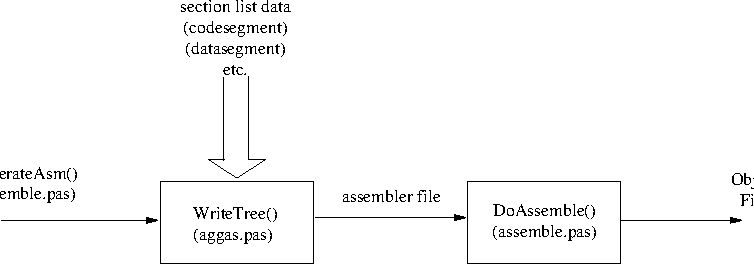
\epsfig{file=arch11.png,width=\textwidth}
\else
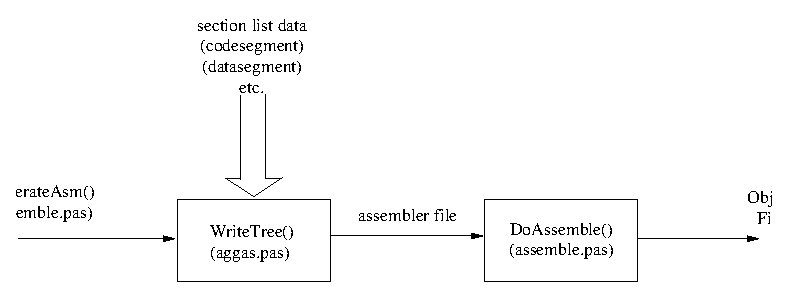
\includegraphics[width=5.67in,height=2.17in]{arch11.eps}
\fi
\label{fig11}
\caption{Assembler generation organisation}
\end{figure}

% FIXME
% If I don't do this, the assembler node table has a problem.
\clearpage

The different possible sections which are output are as follows:

\begin{center}
Section lists for the assembler output
\end{center}

\begin{longtable}{|l|p{10cm}|}
\hline
Internal section name & Description \\
\hline
\endhead
\hline
\endfoot
exparasmlist    & temporary list \\
datasegment     & initialized variables \\
codesegment     & instructions and general code directives \\
debuglist       & debugging information \\
withdebuglist   & ??????????????? \\
consts          & read only constants \\
importsection   & imported symbols \\
exportsection   & exported symbols \\
resourcesection & Resource data \\
rttilist        & runtime type information data \\
resourcestringlist& resource string data
\end{longtable}

The following directives for the abstract assembler currently exist:

Abstract assembler node types:

\begin{longtable}{|l|p{10cm}|}
\hline
Node entry Type   & Description \\
\hline
\endhead
\hline
\endfoot
ait{\_}none&
    This entry in the linked list is invalid (this should
    normally never occur) \\
ait{\_}direct&
    Direct output to the resulting assembler file (as string) \\
ait{\_}string&
    Shortstring with a predefined length \\
ait{\_}label&
    Numbered assembler label used for jumps \\
ait{\_}comment&
    Assembler output comment \\
ait{\_}instruction&
    Processor specific instruction \\
ait{\_}datablock&
    Unitialized data block (BSS) \\
ait{\_}symbol&
    Entry represents a symbol (exported, imported, or other public
    symbol type) \newline
    Possible symbol types : NONE, EXTERNAL, LOCAL and GLOBAL \newline
    eg : A symbol followed by an ait{\_}const{\_}32bit \\
ait{\_}symbol{\_}end &
    Symbol end (for example the end of a routine) \\
ait{\_}const{\_}32bit&
    Initialized 32-bit constant (without a symbol) \\
ait{\_}const{\_}16bit&
    Initialized 16-bit constant (without a symbol) \\
ait{\_}const{\_}8bit&
    Initialized 8-bit constant (without a symbol) \\
ait{\_}const{\_}symbol & ???????????? \\
ait{\_}real{\_}80bit (x86)&
    Initialized 80-bit floating point constant (without symbol) \\
ait{\_}real{\_}64bit&
    Initialized Double IEEE floating point constant (without symbol) \\
ait{\_}real{\_}32bit&
    Initialized Single IEEE floating point constant (without symbol) \\
ait{\_}comp{\_}64bit (x86)&
    Initialized 64-bit floating point integer (without symbol) \\
ait{\_}align&
    Alignment directive \\
ait{\_}section&
    Section directive \\
ait{\_}const{\_}rva (Win32)&  \\
ait{\_}stabn &
    stabs debugging information (numerical value) \\
ait{\_}stabs &
    stabs debugging information (string) \\
ait{\_}force{\_}line&
    stabs debugging line information \\
ait{\_}stab{\_}function{\_}name&
    stabs debug information routine name \\
ait{\_}cut&
    Cut in the assembler files (used for smartlinking) \\
ait{\_}regalloc&
    Debugging information for the register allocator \\
ait{\_}marker  & ???????????? \\
ait{\_}frame (Alpha)&  \\
ait{\_}ent (Alpha)&  \\
ait{\_}labeled{\_}instruction (m68k)&  \\
ait{\_}dummy & Unused - should never appear
\end{longtable}

\section{The Runtime library}
\label{sec:mylabel9}

This section describes the requirements of the internal routines which MUST
be implemented for all relevant platforms to port the system unit to a new
architecture or operating system.

The following defines are available when compiling the runtime library:

\begin{longtable}{|l|p{10cm}|}
\hline
Define Name & Description \\
\hline
\endhead
\hline
\endfoot
i386        & Intel 80x86 family of processors (and compatibles) \\
m68k        & Motorola 680x0 family of processors (excludes coldfire) \\
alpha       & Alpha 21x64 family of processors \\
powerpc     & Motorola / IBM 32-bit family of processors \\
sparc       & SPARC v7 compatible processors
\end{longtable}

\begin{longtable}{|l|p{10cm}|}
\hline
Define name & Description \\
\hline
\endhead
\hline
\endfoot
RTLLITE&
    Removes some extraneous routine from compilation (system unit
    is minimal). Mvdv: Afaik the status of this is unknown \\
DEFAULT{\_}EXTENDED&

    The runtime library routines dealing with fixed point values have the
    \textsf{extended} type instead of the \textsf{real} type. \\
SUPPORT{\_}SINGLE&
    The compiler supports the \textsf{single} floating point precision type \\
SUPPORT{\_}DOUBLE&
    The compiler supports the \textsf{double }floating point precision type \\
SUPPORT{\_}EXTENDED&
    The compiler supports the \textsf{extended }floating point
    precision type \\
SUPPORT{\_}FIXED&
    The compiler supports the \textsf{fixed} floating point precision type \\
HASWIDECHAR&
    The compiler supported the \textsf{widechar} character type \\
INT64&
    The compiler supports 64-bit integer operations \\
MAC{\_}LINEBREAK&
    Text I/O uses Mac styled line break ({\#}13) instead of {\#}13{\#}10 \\
SHORT{\_}LINEBREAK&
    Text I/O uses UNIX styled line breaks ({\#}10) instead of {\#}13{\#}10 \\
EOF{\_}CTRLZ&
    A Ctrl-Z character in a text file is an EOF marker (UNIX mostly) \\
\end{longtable}

The following defines are used for fexpand definitions:

% FIXME Seem to miss a *nix symlink expand behaviour define.
\begin{longtable}{|l|p{10cm}|}
\hline
Define name & Description \\
\hline
\endhead
\hline
\endfoot
FPC{\_}EXPAND{\_}DRIVES&
    Different devices with different names (as drives) are
    supported \par (like DOS, Netware, etc\ldots ) \\
FPC{\_}EXPAND{\_}UNC&
    Universal Naming convention support i.e \par $\backslash \backslash
    < $server-name>$\backslash $<share-name>$\backslash $<directory/filename> \\
UNIX&
    Unix style file names \\
FPC{\_}EXPAND{\_}VOLUMES&
    Volume names (i.e. drive descriptions longer than 1
    character) are supported. \\
FPC{\_}EXPAND{\_}TILDE&
    Replaces the $\sim $ character, with the `HOME' directory
    (mostly on UNIX platforms) \\
\end{longtable}

The following defines some debugging routines for the runtime library:

\begin{longtable}{|l|p{10cm}|}
\hline
Define Name & Description \\
\hline
\endhead
\hline
\endfoot
DEFINE NAME     & Description \\
ANSISTRDEBUG    & Add Debug routines for ansi string support \\
EXCDEBUG        & Add Debug routines for exception debugging \\
LOGGING         & Log the operations to a file \\
\end{longtable}

\subsection{Operating system hooks}
\label{subsec:operating}

This section contains information on all routines which should be hooked and
implemented to be able to compile and use the system unit for a new
operating system:

\begin{functionl}{System{\_}Exit}{systemexit}
\Declaration
procedure System{\_}Exit;
\Description
This routine is internally called by the system unit when the application
exits.
\Notes
This routine should actually exit the application. It should exit with the
error code specified in the \textsf{ExitCode} variable.
\Algorithm
Exit application with ExitCode value.
\end{functionl}

\begin{function}{ParamCount}
\Declaration
Function ParamCount : Longint;
\end{function}

\begin{procedure}{Randomize}
\Declaration
Procedure Randomize;
\Description
This routine initializes the built-in random generator with a random value.
\Notes
This routine is used by random
\Algorithm
Randseed := pseudo random 32-bit value
\end{procedure}

\begin{function}{GetHeapStart}
\Declaration
Function GetHeapStart : Pointer;
\Description
This routine should return a pointer to the start of the heap area.
\Notes
GetHeapStart := address of start of heap.
\end{function}

\begin{function}{GetHeapSize}
\Declaration
Function GetHeapSize : Longint;
\Description
This routine should return the total heap size in bytes
\Parameters
\Algorithm
GetHeapSize := total size of the initial heap area.
\end{function}

\begin{function}{sbrk}
\Declaration
Function sbrk(Size : Longint): Longint;
\Description
\end{function}

\begin{procedurel}{Do{\_}Close}{doclose}
\Declaration
Procedure Do{\_}Close(Handle : Longint);
\Description
This closes the file specified of the specified handle number.
\Parameters
handle = file handle of file to close
\Notes
This routine should close the specified file.
\end{procedurel}

\begin{functionl}{Do{\_}Erase}{doerase}
\Declaration
procedure Do{\_}Erase(p: pchar);
\Description
This erases the file specifed by p.
\Parameters
p = name of the file to erase
\Notes
\end{functionl}

The following variables should also be defined for each new operating
system, they are used by external units:

\noindent
argc : The number of command line arguments of the program

\noindent
argv : A pointer to each of the command line arguments (an array of pchar
pointers)

\subsection{CPU specific hooks}
\label{subsec:mylabel9}

The following routines must absolutely be implemented for each processor, as
they are dependent on the processor:

\subsubsection{FPC{\_}SETJMP}
\label{subsubsec:mylabel30}

\begin{function}{SetJmp}
\Declaration
function SetJmp (Var S : Jmp{\_}Buf) : Longint;
\Description
A call to SetJmp(), saves the calling environment in its \textsf{s} argument
for later use by \textsf{longjmp()}. Called by the code generator in
exception handling code. The return value should be zero.
\Notes
This routine should save / restore all used registers (except the
accumulator which should be cleared).
\end{function}

\subsubsection{FPC{\_}LONGJMP}
\label{subsubsec:mylabel31}

\subsubsection{function SPtr()}
\label{subsubsec:function}

\subsubsection{function Get{\_}Caller{\_}Frame(framebp:longint):longint;}
\label{subsubsec:mylabel32}

\subsubsection{function Get{\_}Caller{\_}Addr(framebp:longint):longint;}
\label{subsubsec:mylabel33}

\subsubsection{function Get{\_}Frame:longint;}
\label{subsubsec:mylabel34}

\subsubsection{function Trunc()}
\label{subsubsec:mylabel35}

\subsection{String related}
\label{subsec:string}

\subsubsection{FPC{\_}SHORTSTR{\_}COPY}
\label{subsubsec:mylabel36}

\begin{procedurel}{Int{\_}StrCopy}{intstrcopy}
\Declaration
Procedure Int{\_}StrCopy(len:longint;sstr,dstr:pointer);
\Description
This routine copies the string pointed to by the address in sstr, to the
string pointed in the destination. The old string is overwritten, and the
source string will be truncated to make it fit in destination if the length
of the source is greater then destination string len (the len parameter).
\Parameters
len = maximum length to copy (the destination string length) \par
sstr = pointer to source shortstring \par
dstr = point to destination shortstring
\Notes
Called by code generator when a string is assigned to another string.
\end{procedurel}

\subsubsection{FPC{\_}SHORTSTR{\_}COMPARE}
\label{subsubsec:mylabel37}

\begin{functionl}{Int{\_}StrCmp}{intstrcmp}
\Declaration
Function Int{\_}StrCmp(dstr,sstr:pointer) : longint;
\Description
The routine compares two shortstrings, and returns 0 if both are equal, 1 if
\textsf{dest} is greater then \textsf{src}, otherwise it returns --1.
\Notes
Both pointers must point to shortstrings. Length checking must be performed
in the routine.
\end{functionl}

\subsubsection{FPC{\_}SHORTSTR{\_}CONCAT}
\label{subsubsec:mylabel38}

\begin{procedurel}{Int{\_}StrConcat}{intstrconcat}
\Declaration
Procedure Int{\_}StrConcat(src,dest:pointer);
\Description
This routine appends the string pointed to by \textsf{src} to the end of the
string pointed to by \textsf{dest}.
\Parameters
src  = pointer to shortstring to append to dest \par
dest = pointer to shortstring to receive appended string
\Notes
Both pointers must point to shortstrings. In the case where the src string
length does not fit in dest, it is truncated.
\Algorithm
\begin{lstlisting}{}
if src =nil or dest = nil then 
 exit routine;
if (src string length + dest string length) > 255 then
 number of bytes to copy = 255 -- dest string length
else
 number of bytes to copy = src string length;
copy the string data (except the length byte)
dest string length = dest string length + number of bytes to copied
\end{lstlisting}
\end{procedurel}

\subsubsection{FPC{\_}ANSISTR{\_}CONCAT}
\label{subsubsec:mylabel39}

\begin{procedurel}{AnsiStr{\_}Concat}{ansistrconcat}
\Declaration
Procedure AnsiStr{\_}Concat(s1,s2:Pointer;var s3:Pointer);
\Description
This routine appends \textsf{s1}+\textsf{s2} and stores the result at the
address pointed to by \textsf{s3}.
\Notes
All pointers must point to ansistrings. 
\end{procedurel}

\subsubsection{FPC{\_}ANSISTR{\_}COMPARE}
\label{subsubsec:mylabel40}

\begin{functionl}{AnsiStr{\_}Compare}{ansistrcompare}
\Declaration
Function AnsiStr{\_}Compare(s1,s2 : Pointer): Longint;
\Description
The routine compares two ansistrings, and returns 0 if both are equal, 1 if
\textsf{s1} is greater then \textsf{s2}, otherwise it returns --1.
\Parameters
Both pointers must point to ansistrings.
\end{functionl}

\subsubsection{FPC{\_}ANSISTR{\_}INCR{\_}REF }
\label{subsubsec:mylabel41}

\begin{procedurel}{AnsiStr{\_}Incr{\_}Ref}{ansistrincrref}
\Declaration
procedure AnsiStr{\_}Incr{\_}Ref (var s : Pointer);
\Description
This routine simply increments the ANSI string reference count, which is
used for garbage collection of ANSI strings.
\Parameters
s = pointer to the ansi string (including the header structure)
\end{procedurel}

\subsubsection{FPC{\_}ANSISTR{\_}DECR{\_}REF }
\label{subsubsec:mylabel42}

\begin{procedurel}{AnsiStr{\_}Decr{\_}Ref}{ansistrdecrref}
\Declaration
procedure AnsiStr{\_}Decr{\_}Ref (Var S : Pointer);
\Parameters
s = pointer to the ansi string (including the header structure)
\Algorithm
Decreases the internal reference count of this non constant ansistring; If
the reference count is zero, the string is deallocated from the
heap.
\end{procedurel}

\subsubsection{FPC{\_}ANSISTR{\_}ASSIGN }
\label{subsubsec:mylabel43}

\begin{functionl}{AnsiStr{\_}Assign}{ansistrassign}
\Declaration
Procedure AnsiStr{\_}Assign (var s1 : Pointer;s2 : Pointer);
\Parameters
s1 = address of ANSI string to be assigned to  \par
s2 = address of ANSI string which will be assigned
\Algorithm
Assigns S2 to S1 (S1:=S2), also by the time decreasing the reference count
to S1 (it is no longer used by this variable).
\end{functionl}

\subsubsection{FPC{\_}PCHAR{\_}TO{\_}SHORTSTR}
\label{subsubsec:mylabel44}

\begin{function}{StrPas}
\Declaration
Function StrPas(p:pChar):ShortString;
\Description
Copies and converts a null-terminated string (pchar) to a shortstring with
length checking.
\Parameters
p = pointer to null terminated string to copy
\Notes
Length checking is performed. Verifies also p=nil, and if so sets the
shortstring length to zero. Called by the type conversion generated code of
code generator.
\Algorithm
\begin{lstlisting}{}
if p=nil then
 string length =0
else
 string length =string length(p)
 if string length>255 then
  string length = 255
 if string length>0 then
  Copy all characters of pchar array to string (except length byte)
\end{lstlisting}
\end{function}

\subsubsection{FPC{\_}SHORTSTR{\_}TO{\_}ANSISTR}
\label{subsubsec:mylabel45}

\begin{functionl}{FPC{\_}ShortStr{\_}To{\_}AnsiStr}{fpcshortstrtoansistr}
\Notes
Called by the type conversion generated code of code generator.
\end{functionl}

\subsubsection{FPC{\_}STR{\_}TO{\_}CHARARRAY}
\label{subsubsec:mylabel46}

\begin{procedurel}{Str{\_}To{\_}CharArray}{strtochararray}
\Declaration
procedure Str{\_}To{\_}CharArray(StrTyp, ArraySize: Longint; src,dest: pChar);
\Description
Converts a string to a character array (currently supports both shortstring and ansistring types). Length checking is performed, and copies up to \textsf{arraysize} elements to dest.
\Parameters
strtyp = Indicates the conversion type to do (0 = shortstring, 1 =
ansistring, 2 = longstring, 3 = widestring) \\
arraysize = size of the destination array \par
src = pointer to source string \par
dest = pointer to character array
\Notes
Called by the type conversion generated code of code generator when
converting a string to an array of char. If the size of the string is less
then the size of the array, the rest of the array is filled with zeros.
\end{procedurel}

\subsubsection{FPC{\_}CHARARRAY{\_}TO{\_}SHORTSTR}
\label{subsubsec:mylabel47}

\begin{function}{StrCharArray}
\Declaration
Function StrCharArray(p:pChar; l : Longint):ShortString;
\Description
Copies a character array to a shortstring with length checking (upto 255
characters are copied)
\Parameters
p = Character array pointer \par
l = size of the array
\Notes
Called by the type conversion generated code of code generator when
converting an array of char to a shortstring.
\Algorithm
\begin{lstlisting}{}
if size of array >= 256 then 
 length of string =255
else
 if size of array < 0 then
  length of string = 0
 else
  length of string = size of array
 Copy all characters from array to shortstring
\end{lstlisting}
\end{function}

\subsubsection{FPC{\_}CHARARRAY{\_}TO{\_}ANSISTR}
\label{subsubsec:mylabel48}

\begin{functionl}{Fpc{\_}Chararray{\_}To{\_}AnsiStr}{chararraytoansistr}
\Notes
Called by the type conversion generated code of code generator when converting an array of char to an ansistring.
\end{functionl}

\subsubsection{FPC{\_}CHAR{\_}TO{\_}ANSISTR}
\label{subsubsec:mylabel49}

\begin{functionl}{Fpc{\_}Char{\_}To{\_}AnsiStr}{fpcchartoansistr}
\Notes
Called by the type conversion generated code of code generator when
converting a char to an ansistring.
\end{functionl}

\subsubsection{FPC{\_}PCHAR{\_}TO{\_}ANSISTR}
\label{subsubsec:mylabel50}

\begin{functionl}{Fpc{\_}pChar{\_}To{\_}AnsiStr}{fpcpchartoansistr}
\Notes
Called by the type conversion generated code of code generator when
converting a pchar to an ansistring.
\end{functionl}

% maybe not necessary anymore (since the amount of tables decreased
% by "macrofying" the procedure definitions)
\ifpdf
 \clearpage
\fi

\subsection{Compiler runtime checking}
\label{subsec:compiler}

\subsubsection{FPC{\_}STACKCHECK}
\label{subsubsec:mylabel51}

\begin{procedurel}{Int{\_}StackCheck}{intstackcheck}
\Declaration
procedure int{\_}stackcheck (stack{\_}size:longint;
\Description
This routine is used to check if there will be a stack overflow when trying
to allocate stack space from the operating system. The routine must preserve
all registers. In the case the stack limit is reached, the routine calls the
appropriate error handler.
\Parameters
stack{\_}size = The amount of stack we wish to allocate
\Notes
Inserted in the entry code of a routine in the {\{}{\$}S+{\}} state by the code generator
\Algorithm
\begin{lstlisting}{}
if ((StackPointer -- stack{\_}size) < System.StackLimit) then
 Throw a Runtime error with error code 202 (stack overflow)
\end{lstlisting}
\end{procedurel}

\clearpage
\subsubsection{FPC{\_}RANGEERROR}
\label{subsubsec:mylabel52}

\begin{procedurel}{Int{\_}RangeError}{intrangerror}
\Declaration
procedure Int{\_}RangeError;
\Description
This routine is called when a range check error is detected when executing
the compiled code. This usually simply calls the default error handler, with
the correct runtime error code to produce.
\Parameters
Inserted in code generator when a Runtime error 201 {\{}{\$}R+{\}} should be
generated
\end{procedurel}

\subsubsection{FPC{\_}BOUNDCHECK}
\label{subsubsec:mylabel53}

\begin{procedurel}{Int{\_}BoundCheck}{intboundcheck}
\Declaration
procedure Int{\_}BoundCheck(l : Longint; Range : Pointer);
\Description
This routine is called at runtime in {\$}R+ mode to check if accessing
indexes in a string or array is out of bounds. In this case, the default
error handler is called, with the correct runtime error code to produce.
\Parameters
l = Index we need to check  \par
range = pointer to a structure containing the minimum and maximum allowed
indexes (points to two 32-bit signed values which are the limits of the
array to verify).
\Notes
Inserted in the generated code after assignments, and array indexing to
verify if the result of operands is within range (in the {\{}{\$}R+{\}}
state)
\end{procedurel}

\subsubsection{FPC{\_}OVERFLOW}
\label{subsubsec:mylabel54}

\begin{procedurel}{Int{\_}OverFlow}{intoverflow}
\Declaration
procedure Int{\_}OverFlow;
\Description
This routine is called when an overflow is detected when executing the
compiled code. This usually simply calls the default error handler, with the
correct runtime error code to produce.
\Parameters
Inserted in code generator when a Runtime error 215 {\{}{\$}Q+{\}} should be
generated.
\end{procedurel}

\subsubsection{FPC{\_}CHECK{\_}OBJECT}
\label{subsubsec:mylabel55}

\begin{procedurel}{Int{\_}Check{\_}Object}{intcheckobject}
\Declaration
procedure Int{\_}Check{\_}Object(vmt : Pointer);
\Description
This routine is called at runtime in the {\$}R+ state each time a virtual
method is called. It verifies that the object constructor has been called
first to build the VMT of the object, otherwise it throws an Runtime error 210.
\Parameters
vmt = Current value of the SELF register
\Notes
Call inserted by the code generator before calling the virtual method. This
routine should save / restore all used registers.
\Algorithm
\begin{lstlisting}{}
if vmt = nil or size of method table =0 then
 Throw a Runtime error with error code 210 (object not initialized)
\end{lstlisting}
\end{procedurel}

\subsubsection{FPC{\_}CHECK{\_}OBJECT{\_}EXT}
\label{subsubsec:mylabel56}

\begin{procedurel}{Int{\_}Check{\_}Object{\_}Ext}{intcheckobjectext}
\Declaration
procedure Int{\_}Check{\_}Object{\_}Ext(vmt, expvmt : pointer);
\Description
This routine is called at runtime when extended object checking is enabled (on the command line) and a virtual method is called. It verifies that the object constructor has been called first to build the VMT of the object, otherwise it throws an Runtime error 210, and furthermore it check that the object is actually a descendant of the parent object, otherwise it returns a Runtime error 220.
\Parameters
vmt = Current value of the SELF register \par
expvmt = Pointer to TRUE object definition
\Notes
Call inserted by the code generator before calling the virtual method. \par
This routine should save / restore all used registers.
\Algorithm
\begin{lstlisting}{}
if vmt = nil or size of method table =0 then
 Throw a Runtime error with error code 210 (object not initialized)
Repeat
 If SELF (VMT) <> VMT Address (expvmt) Then
  Get Parent VMT Address
 Else
  Exit; 
until no more  ent; 
Throw a Runtime error with error code 220 (Incorrect object reference)
\end{lstlisting}
\end{procedurel}

\subsubsection{FPC{\_}IO{\_}CHECK}
\label{subsubsec:mylabel57}

\begin{procedurel}{Int{\_}IOCheck}{intiocheck}
\Declaration
procedure Int{\_}IOCheck(addr : longint);
\Description
This routine is called after an I/O operation to verify the success of the
operation when the code is compiled in the {\$}I+ state.
\Parameters
addr = currently unused
\Algorithm
Check last I/O was successful, if not call error handler.
\end{procedurel}

\subsubsection{FPC{\_}HANDLEERROR}
\label{subsubsec:mylabel58}

\begin{procedure}{HandleError}
\Declaration
procedure HandleError (Errno : longint);
\Description
This routine should be called to generate a runtime error either from one of
the system unit routines or the code generator.
\Parameters
Errno = Runtime error to generate
\Notes
This routine calls the appropriate existing error handler with the specified
error code.
\Algorithm
\end{procedure}

\subsubsection{FPC{\_}ASSERT}
\label{subsubsec:mylabel59}

\begin{procedurel}{Int{\_}Assert}{intassert}
\Declaration
procedure Int{\_}Assert(Const Msg,FName:Shortstring;LineNo,ErrorAddr:Longint);
\Description
This routine is called by the code generator in an assert statement. When
the assertion fails, this routine is called.
\Parameters 
msg = string to print  \par
Fname = Current filename of source \par
LineNo = Current line number of source \par
ErrorAddr = Address of assertion failure
\end{procedurel}

\subsection{Exception handling}
\label{subsec:exception}

\subsubsection{FPC{\_}RAISEEXCEPTION}
\label{subsubsec:mylabel60}

\begin{function}{RaiseExcept}
\Declaration
function RaiseExcept (Obj : Tobject; AnAddr,AFrame : Pointer) : Tobject;
\Description
Called by the code generator in the raise statement to raise an exception. 
\Parameters
Obj = Instance of class exception handler \par
AnAddr = Address of exception \par
Aframe = Exception frame address
\Notes
REGISTERS NOT SAVED???????????
\end{function}

\subsubsection{FPC{\_}PUSHEXCEPTADDR}
\label{subsubsec:mylabel61}

\begin{function}{PushExceptAddr}
\Declaration
function PushExceptAddr (Ft: Longint): PJmp{\_}buf ;
\Description
This routine should be called to save the current caller context to be used
for exception handling, usually called in the context where ANSI strings are
used (they can raise exceptions), or in a try..finally or on statements to
save the current context.
\Parameters 
Ft = Indicates the frame type on the stack (1= Exception frame or 2=Finalize
frame)
\Algorithm
Adds this item to the linked list of stack frame context information saved.
Allocates a buffer for the jump statement and returns it.
\end{function}

\subsubsection{FPC{\_}RERAISE}
\label{subsubsec:mylabel62}

\begin{procedure}{ReRaise}
\Declaration
procedure ReRaise;
\Notes
REGISTERS NOT SAVED???????????
\end{procedure}

\subsubsection{FPC{\_}POPOBJECTSTACK}
\label{subsubsec:mylabel63}

\begin{function}{PopObjectStack}
\Declaration
function PopObjectStack : TObject;
\Description
This is called by the code generator when an exception occurs, it is used to
retrieve the exception handler object from the context information.
\Notes
REGISTERS NOT SAVED???????????
\end{function}

\subsubsection{FPC{\_}POPSECONDOBJECTSTACK}
\label{subsubsec:mylabel64}

\begin{function}{PopSecondObjectStack}
\Declaration
function PopSecondObjectStack : TObject;
\Description
This is called by the code generator when a double exception occurs, it is
used to retrieve the second exception handler object from the context
information.
\Notes
REGISTERS NOT SAVED???????????
\end{function}

\subsubsection{FPC{\_}DESTROYEXCEPTION}
\label{subsubsec:mylabel65}

\begin{procedure}{DestroyException}
\Declaration
Procedure DestroyException(o : TObject);
\Description
This routine is called by the code generator after the exception handling
code is complete to destroy the exception object.
\Parameters 
o = Exception handler object reference
\Notes
REGISTERS NOT SAVED?????????????
\end{procedure}

\subsubsection{FPC{\_}POPADDRSTACK}
\label{subsubsec:mylabel66}

\begin{procedure}{PopAddrStack}
\Declaration
procedure PopAddrStack;
\Description
Called by the code generator in the finally part of a try statement to
restore the stackframe and dispose of all the saved context information.
\Notes
REGISTERS NOT SAVED??????????
\end{procedure}

\subsubsection{FPC{\_}CATCHES}
\label{subsubsec:mylabel67}

\begin{function}{Catches}
\Declaration
function Catches(Objtype : TExceptObjectClass) : TObject;
\Description
This routine is called by the code generator to get the exception handler
object. ?????????????????
\Parameters
ObjType = The exception type class
\Notes
REGISTERS NOT SAVED??????????
\end{function}

\subsubsection{FPC{\_}GETRESOURCESTRING}
\label{subsubsec:mylabel68}

\begin{function}{GetResourceString}
\Declaration
function GetResourceString(Const TheTable: TResourceStringTable;Index : longint) : AnsiString;
\Description
Called by code generator when a reference to a resource string is made. This
routine loads the correct string from the resource string section and
returns the found string (or `' if not found).
\Parameters
TheTable = pointer to the resource string table \par
Index = Index in the resource string table.
\end{function}

\subsection{Runtime type information}
\label{subsec:runtime}

\subsubsection{FPC{\_}DO{\_}IS}
\label{subsubsec:mylabel69}

\begin{functionl}{Int{\_}Do{\_}Is}{intdois}
\Declaration
Function Int{\_}Do{\_}Is(AClass : TClass;AObject : TObject) : Boolean;
\Description
If \textsf{aclass} is of type \textsf{aobject}, returns TRUE otherwise
returns FALSE.
\Parameters
aclass = class type reference \par
aobject = Object instance to compare against
\Notes
This is called by the code generator when the \textsf{is} operator is used.
\Algorithm
\end{functionl}

\subsubsection{FPC{\_}DO{\_}AS}
\label{subsubsec:mylabel70}

\begin{procedurel}{Int{\_}Do{\_}As}{intdoas}
\Declaration
Procedure Int{\_}Do{\_}As(AClass : TClass;AObject : TObject)
\Description
Typecasts \textsf{aclass} as \textsf{aobject}, with dynamic type checking.
If the object is not from the correct type class, a runtime error 219 is
generated. Called by the code generator for the \textsf{as} statement.
\Parameters
aclass = Class to typecast to \par
aobject = Object to typecast
\end{procedurel}

\subsubsection{FPC{\_}INITIALIZE }
\label{subsubsec:mylabel71}

\begin{procedure}{Initialize}
\Declaration
Procedure Initialize (Data,TypeInfo : Pointer);
\Description
\Parameters
data = pointer to the data to initialize \par
typeinfo = pointer to the type information for this data
\Notes
This routine should save / restore all used registers.
\Algorithm
Initializes the class data for runtime typed values
\end{procedure}

\subsubsection{FPC{\_}FINALIZE}
\label{subsubsec:mylabel72}

\begin{procedure}{Finalize}
\Declaration
procedure Finalize (Data,TypeInfo: Pointer);
\Description
Called by code generator if and only if the reference to finalize <> nil.
\Parameters
data = point to the data to finalize \par
typeinfo = Pointer to the type information of this data
\Notes
This routine should save / restore all used registers. Finalizes and frees
the heap class data for runtime typed values (decrements the reference
count)
\end{procedure}

\subsubsection{FPC{\_}ADDREF}
\label{subsubsec:mylabel73}

\begin{procedure}{AddRef}
\Declaration
Procedure AddRef (Data,TypeInfo : Pointer);
\Description
Called by the code generator for class parameters (property support) of type
const or value in parameters, to increment the reference count of ANSI
strings.
\Notes
This routine should save / restore all used registers. This routine can be
called recursively with a very deep nesting level, an assembler
implementation in suggested.
\end{procedure}

\subsubsection{FPC{\_}DECREF}
\label{subsubsec:mylabel74}

\begin{procedure}{DecRef}
\Declaration
Procedure DecRef (Data, TypeInfo : Pointer);
\Description
Called by the code generator for class parameters (property support) of type
const or value parameters, to decrement the reference count. of ANSI
strings.
\Parameters
\Notes
This routine should save / restore all used registers. This routine can be
called recursively with a very deep nesting level, an assembler
implementation in suggested.
\end{procedure}

\subsection{Memory related}
\label{subsec:memory}

\clearpage
\subsubsection{FPC{\_}GETMEM}
\label{subsubsec:mylabel75}

\begin{procedure}{GetMem}
\Declaration
procedure GetMem(Var p:Pointer;Size:Longint);
\end{procedure}

\subsubsection{FPC{\_}FREEMEM}
\label{subsubsec:mylabel76}

\begin{procedure}{FreeMem}
\Declaration
Procedure FreeMem(Var P:Pointer;Size:Longint);
\end{procedure}

\subsubsection{FPC{\_}CHECKPOINTER}
\label{subsubsec:mylabel77}

\begin{function}{CheckPointer}
\Declaration
Procedure CheckPointer(p : Pointer);
\Description
Called by the code generator when a pointer is referenced in heap debug
mode. Verifies that the pointer actually points in the heap area.
\Parameters
p = pointer to check
\Notes
This routine should save /restore all used registers.
\end{function}

\subsubsection{FPC{\_}DO{\_}EXIT}
\label{subsubsec:mylabel78}

\begin{procedurel}{Do{\_}Exit}{doexit}
\Declaration
procedure Do{\_}Exit;
\Description
Called by code generator at the end of the program entry point.
\Notes
Called to terminate the program
\Algorithm
Call all unit exit handlers. \par
Finalize all units which have a finalization section \par
Print runtime error in case of error\par
Call OS-dependant system{\_}exit routine
\end{procedurel}

\subsubsection{FPC{\_}ABSTRACTERROR}
\label{subsubsec:mylabel79}

\begin{function}{AbstractError}
\Declaration
procedure AbstractError;
\Description
The code generator allocates a VMT entry equal to this routine address when
a method of a class is declared as being abstract. This routine simply calls
the default error handler.
\Algorithm
Throw a Runtime error with error code 211 (Abstract call)
\end{function}

\subsubsection{FPC{\_}INITIALIZEUNITS}
\label{subsubsec:mylabel80}

\begin{function}{InitializeUnits}
\Declaration
\Description
Called by the code generator in the main program, this is only available if
an \textsf{initialization} section exists in one of the units used by the
program.
\end{function}

\subsubsection{FPC{\_}NEW{\_}CLASS (assembler)}
\label{subsubsec:mylabel81}

\begin{procedurel}{int{\_}new{\_}class}{intnewclass}
\Description
This routine will call the TObject.InitInstance() routine to
instantiate a class (Delphi-styled class) and allocate the memory for all
fields of the class.

On entry the self{\_}register should be valid, and should point either to
nil, for a non-initialized class, or to the current instance of the class.
The first parameter on the top of the stack should be a pointer to the VMT
table for this class(????).
\end{procedurel}

\subsubsection{FPC{\_}HELP{\_}DESTRUCTOR}
\label{subsubsec:mylabel82}

Could be implemented in ASM directly with register parameter passing.

\begin{procedurel}{Int{\_}Help{\_}Destructor}{inthelpdestructor}
\Declaration
Procedure Int{\_}Help{\_}Destructor(Var {\_}Self : Pointer; Vmt : Pointer; Vmt{\_}Pos : Cardinal);
\Description
Frees the memory allocated for the object fields, and if the object had a
VMT field, sets it to nil.
\Parameters
self = pointer to the object field image in memory \par
vmt = pointer to the the actual vmt table (used to get the size of the object) \par
vmt{\_}pos = offset in the object field image to the vmt pointer field
\Notes
This routine should / save restore all used registers.
\Algorithm
\begin{lstlisting}{}
if self = nil then
 exit
set VMT field in object field image ,if present, to nil
Free the allocated heap memory for the field objects
set Self = nil
\end{lstlisting}
\end{procedurel}

\subsubsection{FPC{\_}HELP{\_}CONSTRUCTOR}
\label{subsubsec:mylabel83}

Could be implemented in ASM directly with register parameter passing.

\begin{functionl}{Int{\_}Help{\_}Constructor}{inthelpconstructor}
\Declaration
function Int{\_}Help{\_}Constructor(Var {\_}self : Pointer; Var VMT : Pointer; Vmt{\_}Pos : Cardinal):Pointer;
\Description
Allocates the memory for an object's field, and fills the object fields with
zeros. Returns the newly allocated self{\_}pointer
\Parameters
self = pointer to the object field image in memory \par
vmt = pointer to the the actual vmt table (used to get the size of the object) \par
vmt{\_}pos = offset in the object field image to the vmt pointer field
\Notes
The self{\_}pointer register should be set appropriately by the code
generator to the allocated memory (self parameter)
\Algorithm
Self = Allocate Memory block for object fields \par
Fill the object field image with zeros\par
Set the VMT field in allocated object to VMT pointer
\end{functionl}

\subsubsection{FPC{\_}HELP{\_}FAIL{\_}CLASS}
\label{subsubsec:mylabel84}

\begin{functionl}{Help{\_}Fail{\_}Class}{inthelpfileclass}
\Description
Inserted by code generator after constructor call. If the constructor failed
to allocate the memory for its fields, this routine will be called.
\end{functionl}

\subsubsection{FPC{\_}HELP{\_}FAIL}
\label{subsubsec:mylabel85}

\begin{functionl}{Help{\_}Fail}{HelpFail}
\Description
Inserted by code generator after constructor call. If the constructor failed
to allocate the memory for its fields, this routine will be called.
\end{functionl}

\subsection{Set handling}
\label{subsec:mylabel10}

\subsubsection{FPC{\_}SET{\_}COMP{\_}SETS}
\label{subsubsec:mylabel86}

\begin{functionl}{Do{\_}Comp{\_}Sets}{docompsets}
\Declaration
function Do{\_}Comp{\_}Sets(Set1,Set2 : Pointer): Boolean;
\Description
This routine compares if set1 and set2 are exactly equal and returns 1 if
so, otherwise it returns false.
\Parameters
set1 = Pointer to 32 byte set to compare \par
set2 = Pointer to 32 byte set to compare
\Notes
Both pointers must point to normal sets.
\end{functionl}

\subsubsection{FPC{\_}SET{\_}CONTAINS{\_}SET}
\label{subsubsec:mylabel87}

\begin{procedurel}{Do{\_}Contains{\_}Sets}{docontainssets}
\Declaration
Procedure Do{\_}Contains{\_}Sets(Set1,Set2 : Pointer): Boolean;
\Description
Returns 1 if set2 contains set1 (That is all elements of set2 are in set1).
\Parameters
set1 = Pointer to 32 byte set to verify \par
set2 = Pointer to 32 byte set to verify
\Notes
Both pointers must point to normal sets.
\end{procedurel}

\subsubsection{FPC{\_}SET{\_}CREATE{\_}ELEMENT}
\label{subsubsec:mylabel88}

\begin{procedurel}{Do{\_}Create{\_}Element}{docreateelement}
\Declaration
procedure Do{\_}Create{\_}Element(p : Pointer; b : Byte);
\Description
Create a new normal set in the area pointed to by \textsf{p} and add the
element value \textsf{b} in that set.
\Parameters
p = pointer to area where the 32 byte set will be created \par
b = bit value within that set which must be set
\Notes
This works on normal sets only.
\Algorithm
Zero the area pointed to by p \par
Set the bit number b to 1
\end{procedurel}

\subsubsection{FPC{\_}SET{\_}SET{\_}RANGE}
\label{subsubsec:mylabel89}

\begin{procedurel}{Do{\_}Set{\_}Range}{dosetrange}
\Declaration
Procedure Do{\_}Set{\_}Range(P : Pointer;l,h : Byte);
\Description
Sets the bit values within the \textsf{l} and \textsf{h }bit ranges in the
normal set pointed to by \textsf{p}
\Parameters
p = pointer to area where the 32 bytes of the set will be updated \par
l = low bit number value to set \par
h = high bit number value to set
\Notes
This works on normal sets only.
\Algorithm
Set all bit numbers from l to h in set p
\end{procedurel}

\subsubsection{FPC{\_}SET{\_}SET{\_}BYTE}
\label{subsubsec:mylabel90}

\begin{procedurel}{Do{\_}Set{\_}Byte}{dosetbyte}
\Declaration
procedure Do{\_}Set{\_}Byte(P : Pointer;B : byte);
\Description
Add the element \textsf{b} in the normal set pointed to by \textsf{p}
\Parameters
p = pointer to 32 byte set \par
b = bit number to set
\Notes
This works on normal sets only. The intel 80386 version of the compiler does
not save the used registers, therefore, in that case, it must be done in the
routine itself.
\Algorithm
Set bit number b in p
\end{procedurel}

\subsubsection{FPC{\_}SET{\_}SUB{\_}SETS}
\label{subsubsec:mylabel91}

\begin{procedurel}{Do{\_}Sub{\_}Sets}{dosubsets}
\Declaration
Procedure Do{\_}Sub{\_}Sets(Set1,Set2,Dest:Pointer);
\Description
Calculate the difference between \textsf{set1} and \textsf{set2}, setting
the result in \textsf{dest}.
\Parameters
set1 = pointer to 32 byte set \par
set2 = pointer to 32 byte set \par
dest = pointer to 32 byte set which will receive the result
\Notes
This works on normal sets only. 
\Algorithm
\begin{lstlisting}{}
For each bit in the set do
 dest bit = set1 bit AND NOT set2 bit
\end{lstlisting}
\end{procedurel}

\subsubsection{FPC{\_}SET{\_}MUL{\_}SETS}
\label{subsubsec:mylabel92}

\begin{procedurel}{Do{\_}Mul{\_}Sets}{domulsets}
\Declaration
procedure Do{\_}Mul{\_}Sets(Set1,Set2,Dest:Pointer);
\Description
Calculate the multiplication between \textsf{set1} and \textsf{set2},
setting the result in \textsf{dest}.
\Parameters
set1 = pointer to 32 byte set \par
set2 = pointer to 32 byte set \par
dest = pointer to 32 byte set which will receive the result
\Notes
This works on normal sets only.
\Algorithm
\begin{lstlisting}{}
For each bit in the set do
 dest bit = set1 bit AND set2 bit
\end{lstlisting}
\end{procedurel}

\subsubsection{FPC{\_}SET{\_}SYMDIF{\_}SETS}
\label{subsubsec:mylabel93}

\begin{procedurel}{Do{\_}Symdif{\_}Sets}{dosymdifssets}
\Declaration
Procedure Do{\_}Symdif{\_}Sets(Set1,Set2,Dest:Pointer);
\Description
Calculate the symmetric between \textsf{set1} and \textsf{set2}, setting the
result in \textsf{dest}.
\Parameters
set1 = pointer to 32 byte set \par
set2 = pointer to 32 byte set \par
dest = pointer to 32 byte set which will receive the result
\Notes
This works on normal sets only.
\Algorithm
\begin{lstlisting}{}
For each bit in the set do
 dest bit = set1 bit XOR set2 bit
\end{lstlisting}
\end{procedurel}

\subsubsection{FPC{\_}SET{\_}ADD{\_}SETS}
\label{subsubsec:mylabel94}

\begin{procedurel}{Do{\_}Add{\_}Sets}{doaddsets}
\Declaration
procedure Do{\_}Add{\_}Sets(Set1,Set2,Dest : Pointer);
\Description
Calculate the addition between \textsf{set1} and \textsf{set2}, setting the
result in \textsf{dest}.
\Parameters
set1 = pointer to 32 byte set \par
set2 = pointer to 32 byte set \par
dest = pointer to 32 byte set which will receive the result
\Notes
This works on normal sets only.
\Algorithm
\begin{lstlisting}{}
For each bit in the set do
 dest bit = set1 bit OR set2 bit
\end{lstlisting}
\end{procedurel}

\subsubsection{FPC{\_}SET{\_}LOAD{\_}SMALL}
\label{subsubsec:mylabel95}

\begin{procedurel}{Do{\_}Load{\_}Small}{doloadsmall}
\Declaration
Procedure Do{\_}Load{\_}Small(P : Pointer;L:Longint);
\Description
Load a small set into a 32-byte normal set.
\Parameters
p = pointer to 32 byte set \par
l = value of the small set
\Notes
Called by code generator (type conversion) from small set to large set.
Apart from the first 32 bits of the 32 byte set, other bits are not
modified.
\Algorithm
\begin{lstlisting}{}
For n = bit 0 to bit 31 of l do
 p bit n = l bit n
\end{lstlisting}
\end{procedurel}

\subsubsection{FPC{\_}SET{\_}UNSET{\_}BYTE}
\label{subsubsec:mylabel96}

\begin{procedurel}{Do{\_}Unset{\_}Byte}{dounsetbyte}
\Declaration
Procedure Do{\_}Unset{\_}Byte(P : Pointer;B : Byte);
\Description
Called by code generator to exclude element b from a big 32-byte set pointed
to by p.
\Parameters
p = pointer to 32 byte set \par b = element number to exclude
\Notes
The intel 80386 version of the compiler does not save the used registers,
therefore, in that case, it must be done in the routine itself.
\Algorithm
Clear bit number b in p
\end{procedurel}

\subsubsection{FPC{\_}SET{\_}IN{\_}BYTE}
\label{subsubsec:mylabel97}

\begin{functionl}{Do{\_}In{\_}Byte}{doinbyte}
\Declaration
Function Do{\_}In{\_}Byte(P : Pointer;B : Byte):boolean;
\Description
Called by code generator to verify the existence of an element in a set.
Returns TRUE if b is in the set pointed to by p, otherwise returns FALSE.
\Parameters
p = pointer to 32 byte set \par b = element number to verify
\Notes
This routine should save / restore all used registers.
\Algorithm
Clear bit number b in p
\end{functionl}

\subsection{Optional internal routines}
\label{subsec:optional}

These routines are dependant on the target architecture. They are present in
software if the hardware does not support these features.

They could be implemented in assembler directly with register parameter
passing.

\subsubsection{FPC{\_}MUL{\_}INT64}
\label{subsubsec:mylabel98}

\begin{function}{MulInt64}
\Declaration
function MulInt64(f1,f2 : Int64;CheckOverflow : LongBool) : Int64;
\Description
Called by the code generator to multiply two int64 values, when the hardware
does not support this type of operation. The value returned is the result of
the multiplication.
\Parameters
f1 = first operand \par
f2 = second operand \par
checkoverflow = TRUE if overflow checking should be done
\end{function}

\subsubsection{FPC{\_}DIV{\_}INT64}
\label{subsubsec:mylabel99}

\begin{function}{DivInt64}
\Declaration
function DivInt64(n,z : Int64) : Int64;
\Description
Called by the code generator to get the division two int64 values, when the
hardware does not support this type of operation. The value returned is the
result of the division.
\Parameters
n =numerator \par
z = denominator
\end{function}

\subsubsection{FPC{\_}MOD{\_}INT64}
\label{subsubsec:mylabel100}

\begin{function}{ModInt64}
\Declaration
function ModInt64(n,z : Int64) : Int64;
\Description
Called by the code generator to get the modulo two int64 values, when the
architecture does not support this type of operation. The value returned is
the result of the modulo.
\Parameters
n = numerator \par
z = denominator
\end{function}

\subsubsection{FPC{\_}SHL{\_}INT64}
\label{subsubsec:mylabel101}

\begin{function}{ShlInt64}
\Declaration
Function ShlInt64(Cnt : Longint; Low, High: Longint): Int64;
\Description
Called by the code generator to shift left a 64-bit integer by the specified
amount cnt, when this is not directly supported by the hardware. Returns the
shifted value.
\Parameters
low,high = value to shift (low / high 32-bit value) \par
cnt = shift count
\end{function}

\subsubsection{FPC{\_}SHR{\_}INT64}
\label{subsubsec:mylabel102}

\begin{function}{ShrInt64}
\Declaration
function ShrInt64(Cnt : Longint; Low, High: Longint): Int64;
\Description
Called by the code generator to shift left a 64-bit integer by the specified
amount cnt, when this is not directly supported by the hardware. Returns the
shifted value.
\Parameters
low,high = value to shift (low/high 32-bit values) \par
cnt = shift count
\end{function}

\subsubsection{FPC{\_}MUL{\_}LONGINT}
\label{subsubsec:mylabel103}

\begin{function}{MulLong}
\Declaration
Function MulLong: Longint;
\Description
Called by the code generator to multiply two longint values, when the hardware does not support this type of operation. The value returned is the result of the multiplication.
\Parameters
Parameters are passed in registers.
\Notes
This routine should save / restore all used registers.
\end{function}

\subsubsection{FPC{\_}REM{\_}LONGINT}
\label{subsubsec:mylabel104}

\begin{function}{RemLong}
\Declaration
Function RemLong: Longint;
\Description
Called by the code generator to get the modulo two longint values, when the
hardware does not support this type of operation. The value returned is the
result of the modulo.
\Parameters
Parameters are passed in registers.
\Notes
This routine should save / restore all used registers.
\end{function}

\subsubsection{FPC{\_}DIV{\_}LONGINT}
\label{subsubsec:mylabel105}

\begin{function}{DivLong}
\Declaration
Function DivLong: Longint;
\Description
Called by the code generator to get the division two longint values, when
the hardware does not support this type of operation. The value returned is
the result of the division.
\Parameters
Parameters are passed in registers.
\Notes
This routine should save / restore all used registers.
\end{function}

\subsubsection{FPC{\_}MUL{\_}LONGINT}
\label{subsubsec:mylabel106}

\begin{function}{MulCardinal}
\Declaration
Function MulCardinal: Cardinal;
\Description
Called by the code generator to multiply two cardinal values, when the
hardware does not support this type of operation. The value returned is the
result of the multiplication.
\Parameters
Parameters are passed in registers.
\Notes
This routine should save / restore all used registers.
\end{function}

\subsubsection{FPC{\_}REM{\_}CARDINAL}
\label{subsubsec:mylabel107}

\begin{function}{RemCardinal}
\Declaration
Function RemCardinal : Cardinal;
\Description
Called by the code generator to get the modulo two cardinal values, when the
hardware does not support this type of operation. The value returned is the
result of the modulo.
\Parameters
Parameters are passed in registers.
\Notes
This routine should save / restore all used registers.
\end{function}

\subsubsection{FPC{\_}DIV{\_}CARDINAL}
\label{subsubsec:mylabel108}

\begin{function}{DivCardinal}
\Declaration
Function DivCardinal: Cardinal;
\Description
Called by the code generator to get the division two cardinal values, when
the hardware does not support this type of operation. The value returned is
the result of the division.
\Parameters
Parameters are passed in registers.
\Notes
This routine should save / restore all used registers.
\end{function}

\subsubsection{FPC{\_}LONG{\_}TO{\_}SINGLE}
\label{subsubsec:mylabel109}

\begin{function}{LongSingle}
\Declaration
Function LongSingle: Single;
\Description
Called by the code generator to convert a longint to a single IEEE floating
point value.
\Parameters
Parameters are passed in registers
\Notes
This routine should save / restore all used registers.
\end{function}

FPC{\_}ADD{\_}SINGLE

FPC{\_}SUB{\_}SINGLE

FPC{\_}MUL{\_}SINGLE

FPC{\_}REM{\_}SINGLE

FPC{\_}DIV{\_}SINGLE

FPC{\_}CMP{\_}SINGLE

FPC{\_}SINGLE{\_}TO{\_}LONGINT

\section{Optimizing your code}
\label{sec:optimizing}

\subsection{Simple types}
\label{subsec:simple}

Use the most simple types, when defining and declaring variables, they
require less overhead. Classes, and complex string types (ansi strings and
wide strings) posess runtime type information, as well as more overhead for
operating on them then simple types such as shortstring and simple ordinal
types.

\subsection{constant duplicate merging}
\label{subsec:constant}

When duplicates of constant strings, sets or floating point values are found
in the code, they are replaced by only once instance of the same string, set
or floating point constant which reduces the size of the final executable.

\subsection{inline routines}
\label{subsec:inline}

The following routines of the system unit are directly inlined by the
compiler, and generate more efficient code:

\begin{longtable}{|l|p{7cm}|}
\hline
Prototype& Definition and notes \\
\hline
\endhead
\hline
\endfoot
\textsf{function pi : extended;}& \\
\textsf{function abs(d : extended) : extended;}& \\
\textsf{function sqr(d : extended) : extended;}& \\
\textsf{function sqrt(d : extended) : extended;}& \\
\textsf{function arctan(d : extended) : extended;}& \\
\textsf{function ln(d : extended) : extended;}& \\
\textsf{function sin(d : extended) : extended;}& \\
\textsf{function cos(d : extended) : extended;}& \\
\textsf{function ord(X): longint;}&
   Changes node type to be type compatible \\
\textsf{function lo(X) : byte or word;}&
   Generates 2-3 instruction sequence inline \\
\textsf{function hi(X) : byte or word;}&
   Generates 2-3 instruction sequence inline \\
\textsf{function chr(b : byte) : Char;}&
   Changes node type to be type compatible \\
\textsf{function Length(s : string) : byte;}&
   Generate 2-3 instruction sequence \\
\textsf{function Length(c : char) : byte;}&
   Generates 1 instruction sequence (appx.) \\
\textsf{procedure Reset(var f : TypedFile);}&
   Calls FPC{\_}RESET{\_}TYPED \\
\textsf{procedure rewrite(var f : TypedFile);}&
   Calls FPC{\_}REWRITE{\_}TYPED \\
\textsf{procedure settextbuf(var F : Text; var Buf);}&
   Calls SetTextBuf of runtime library \\
\textsf{procedure writen;}&
   Calls FPC{\_}WRITE{\_}XXXX routines \\
\textsf{procedure writeln;}&
   Calls FPC{\_}WRITE{\_}XXXX routines \\
\textsf{procedure read;}&
   Calls FPC{\_}READ{\_}XXXX routines \\
\textsf{procedure readln;}&
   Calls FPC{\_}READ{\_}XXXX routines \\
\textsf{procedure concat;}&
   Generates a TREE NODES of type addn \\
\textsf{function assigned(var p): boolean;}&
   Generates 1-2 instruction sequence inline \\
\textsf{procedure str(X :[Width [:Decimals]]; var S);}& \\
\textsf{}&  \\
\textsf{function sizeof(X): longint;}&
   Generates 2-3 instruction sequence inline \\
\textsf{function typeof(X): pointer;}&
   Generates 2-3 instruction sequence inline \\
\textsf{procedure val(S;var V; var Code: integer);}& \\
\textsf{function seg(X): longint;}& \\
\textsf{function High(X)}&
   Generates a TREE NODE of type ordconstn \\
\textsf{function Low(X)}&
   Generates a TREE NODE of type ordconstn \\
\textsf{function pred(x)}&
   Generates 2-3 instruction sequence inline \\
\textsf{function succ(X)}&
   Generates 2-3 instruction sequence inline \\
\textsf{procedure inc(var X [ ; N: longint]);}&
   Generate 2-3 instruction sequence inline \\
\textsf{procedure dec(var X [; N:longint]);}&
   Generate 2-3 instruction sequence inline \\
\textsf{procedure include(var s: set of T; I: T);}&
   In the case of a small set : Generates 2-3 instruction sequence inline,
   otherwise calls FPC{\_}SET{\_}SET{\_}BYTE \\
\textsf{procedure exclude(var S : set of T; I: T);}&
   In the case of a small set : Generates 2-3 instruction sequence inline,
   otherwise calls FPC{\_}SET{\_}UNSET{\_}BYTE \\
\textsf{procedure assert(expr : Boolean [; const msg: string]);}&
  Calls the internal routine FPC{\_}ASSERT in the case where the assert fails.\\
\textsf{function addr(X): pointer;}&
  Generates a TREE NODE of type addrn \\
\textsf{function typeInfo(typeIdent): pointer;}&
  Generates 1 instruction sequence inline \\
\end{longtable}

\subsection{temporary memory allocation reuse}
\label{subsec:mylabel11}

When routines are very complex , they may require temporary allocated space
on the stack to store intermediate results. The temporary memory space can
be reused for several different operations if other space is required on the
stack.

\section{Appendix A}
\label{sec:appendix}

This appendix describes the temporary defines when compiling software under
the compiler:

The following defines are defined in FreePascal for v1.0.x, but they will be
removed in future versions, they are used for debugging purposes only:

\begin{itemize}
\item INT64
\item HASRESOURCESTRINGS
\item NEWVMTOFFSET
\item HASINTERNMATH
\item SYSTEMVARREC
\item INCLUDEOK
\item NEWMM
\item HASWIDECHAR
\item INT64FUNCRESOK
\item CORRECTFLDCW
\item ENHANCEDRAISE
\item PACKENUMFIXED
\end{itemize}

NOTE: Currently, the only possible stack alignment are either 2 or 4 if the
target operating system pushes parameters on the stack directly in assembler
(because for example if pushing a long value on the stack while the required
stack alignment is 8 will give out wrong access to data in the actual
routine -- the offset will be wrong).

\printindex
\end{document}
